\input{"preamble_2020_1_07.tex"}
\let\Begin\begin
\let\End\end
\newcommand\wrapenv[1]{#1}

\makeatletter
\def\ScaleWidthIfNeeded{%
 \ifdim\Gin@nat@width>\linewidth
    \linewidth
  \else
    \Gin@nat@width
  \fi
}
\def\ScaleHeightIfNeeded{%
  \ifdim\Gin@nat@height>0.9\textheight
    0.9\textheight
  \else
    \Gin@nat@width
  \fi
}
\makeatother

\setkeys{Gin}{width=\ScaleWidthIfNeeded,height=\ScaleHeightIfNeeded,keepaspectratio}%

\title{
\textbf{
    Real Analysis
  }
  }
\author{D. Zack Garza}
\date{\today}

\begin{document}

\maketitle
% \todo{Insert title and subtitle.}
\tableofcontents


\hypertarget{foreword}{%
\section{Foreword}\label{foreword}}

This are notes from the Fall 2019 Qualifying Exam course for Real
Analysis at the University of Georgia, taught by Professor Neil Lyall.
These were typeset live during each class. If you find any mistakes or
errors, please let me know! Moreover, these may not always reflect
exactly what was said or covered in the course -- I've paraphrased some
things, rephrased others, left out a few bits of more complicated
proofs, and added content here and there.

\hypertarget{summary}{%
\section{Summary}\label{summary}}

\begin{itemize}
\tightlist
\item
  Measure and integration theory with relevant examples from Lebesgue
  integration
\item
  Hilbert spaces (only with regard to \(L^2\)),
\item
  \(L^p\) spaces and the related Riesz representation theorem.
\item
  Hahn, Jordan and Lebesgue decomposition theorems,
\item
  Radon-Nikodym Theorem
\item
  Fubini's Theorem.
\end{itemize}

\emph{Texts}

\begin{itemize}
\tightlist
\item
  Real Analysis, by E. M. Stein and R. Shakarchi
\item
  Real Analysis, by G. B. Folland
\item
  An introduction to measure theory, by Terrence Tao
\item
  Real and Complex Analysis, by W. Rudin
\end{itemize}

\href{http://alpha.math.uga.edu/~lyall/8100Fall2014/index.html}{An old
course page}

\hypertarget{definitions}{%
\subsection{Definitions}\label{definitions}}

\begin{itemize}
\item
  \textbf{Convolution}
  \begin{align*}
  f * g(x)=\int f(x-y) g(y) d y
  \end{align*}
\item
  \textbf{Dilation}
  \begin{align*}
  \phi_{t}(x)=t^{-n} \phi\left(t^{-1} x\right)
  \end{align*}
\item
  The Fourier Transform (todo)
\end{itemize}

\hypertarget{convergence-theorems}{%
\subsection{Convergence Theorems}\label{convergence-theorems}}

\begin{itemize}
\item
  \textbf{Monotone Convergence Theorem (MCT)}: If \(f_n \in L^+\) and
  \(f_n \nearrow f\) a.e., then
  \begin{align*}
  \lim \int f_n 
  = \int \lim f_n = \int f
  \quad \text{i.e.}~~ \int f_n \to \int f
  .\end{align*}
\item
  \textbf{Dominated Convergence Theorem (DCT)}: If \(f_n \in L^1\) and
  \(f_n \to f\) a.e. with \(\abs {f_n} \leq g\) for some \(g\in L^1\),
  then
  \begin{align*}
  \lim \int f_n = \int \lim f_n = \int f \quad \text{i.e.}~~ \int f_n \to \int f
  ,\end{align*}

  and more generally,
  \begin{align*}
  \int \abs{f_n - f} \to 0
  \end{align*}

  \begin{quote}
  Generalized DCT: can relax \(\abs {f_n} < g\) to
  \(\abs{f_n} < g_n \to g\in L^1\).
  \end{quote}
\item
  \textbf{Fatou}: If \(f_n \in L^+\), then
  \begin{align*}
  \int \liminf f_n \leq \liminf \int f_n
  .\end{align*}
\end{itemize}

\hypertarget{inequalities-and-equalities}{%
\subsection{Inequalities and
Equalities}\label{inequalities-and-equalities}}

\begin{itemize}
\item
  \textbf{Reverse Triangle Inequality} \begin{align*}
  \abs{\norm{x} - \norm{y}} \leq \norm{x - y}
  .\end{align*}
\item
  \textbf{Chebyshev's Inequality} \begin{align*}
  \mu(\{x:|f(x)|>\alpha\}) \leq\left(\frac{\|f\|_{p}}{\alpha}\right)^{p}
  .\end{align*}
\item
  ? Inequality
  \begin{align*}
  a^{\lambda} b^{1-\lambda} \leq \lambda a+(1-\lambda) b
  \end{align*} with equality iff \(a=b\).
\item
  \textbf{Holder's Inequality:} For \(p,q\) conjugate exponents,
  \begin{align*}
  \|f g\|_{1} \leq\|f\|_{p}\|g\|_{q}, \quad \text{i.e.} \int \abs{fg} 
  \leq \left( \int \abs{f}^p \right)^{\frac 1 p} \left( \int \abs{g}^q \right)^{\frac 1 q}
  .\end{align*}
\item
  \textbf{Cauchy-Schwarz}: Set \(p=q=2\) in Holder's inequality to
  obtain \begin{align*}
  \abs{\inner{f}{g}} = \norm{fg}_1 \leq \norm{f}_2 \norm{g}_2 
  ,\end{align*} with equality \(\iff f \neq \lambda g\).
\item
  \textbf{Minkowski's Inequality:} For \(1\leq p < \infty\),
  \begin{align*}
  \|f+g\|_{p} \leq\|f\|_{p}+\|g\|_{p}
  \end{align*}
\item
  \textbf{Young's Inequality}: \begin{align*}
  \frac 1 p + \frac 1 q = \frac 1 r + 1 \implies
  \|f \ast g\|_{r} \leq\|f\|_{p}\|g\|_{q}
  .\end{align*}
\end{itemize}

\begin{quote}
Useful specific cases: \begin{align*}
\norm{f\ast g}_1 &\leq \norm{f}_1 \norm{g}_1 \\
\|f * g\|_{p} &\leq\|f\|_{1}\|g\|_{p}, \\
\norm{f\ast g}_\infty &\leq \norm{f}_2 \norm{g}_2 \\
\norm{f\ast g}_\infty &\leq \norm{f}_p \norm{g}_q
.\end{align*}
\end{quote}

\begin{itemize}
\item
  \textbf{Bessel's Inequality:} For \(x\in H\) a Hilbert space and
  \(\theset{e_k}\) an orthonormal sequence, \begin{align*}
  \sum_{k=1}^{\infty}\left|\left\langle x, e_{k}\right\rangle\right|^{2} \leq\|x\|^{2}
  .\end{align*}
\item
  \textbf{Parseval's identity:} Equality in Bessel's inequality,
  attained when \(\theset{e_k}\) is a \emph{basis}, i.e.~it is complete.
\end{itemize}

\hypertarget{other}{%
\subsubsection{Other}\label{other}}

\begin{itemize}
\item
  \textbf{Borel-Cantelli Lemma:} Let \(\{E_k\}\) be a countable
  collection of measurable sets. Then
  \begin{align*}
  \sum_k m(E_k) < \infty \implies \text{ almost every } x\in \RR \text{ is in at most finitely many } E_k
  .\end{align*}
\item
  \textbf{Egorov's Theorem} Let \(E \subseteq \RR^n\) be measurable with
  \(m(E) > 0\) and \(\theset{f_k: E \to \RR}\) be measurable functions
  such that
  \(f(x) \definedas \displaystyle\lim_{k\to\infty} f_k(x) < \infty\)
  exists almost everywhere.

  Then \(f_k \to f\) \emph{almost uniformly}, i.e. \begin{align*}
  \forall\varepsilon > 0, ~\exists F \subseteq E ~\text{closed such that } & 
  m(E\setminus F) < \varepsilon ~\text{ and }~ f_k \mapsvia{u}  f ~\text{on}~ F
  .\end{align*}
\item
  Fubini
\item
  Tonelli
\item
  Fubini/Tonelli
\item
  \textbf{Riemann-Lebesgue Lemma:} \begin{align*}
  f\in L^1 \implies 
  \hat{f}(\xi) \rightarrow 0 \text { as }|\xi| \rightarrow \infty
  .\end{align*}
\item
  \textbf{Differentiating under the integral}:
\end{itemize}

If \(\abs{\dd{}{t}f(x, t)} \leq g(x) \in L^1\), then \begin{align*}
F(t) = \int f(x, t) ~dt 
&\implies \dd{}{t} F(t)\definedas \lim _{h \rightarrow 0} \int \frac{f(x, t+h)-f(x, t)}{h} d x \\
&= \int \dd{}{t} f(x, t) ~dx
.\end{align*}

Let \(h_k \to 0\) be any sequence and define
\(f_k = \frac{f(x, t+h_k)-f(x, t)}{h_k}\), so
\(f_k \converges{\text{pointwise}}\to \dd{}{t}f\).

\hypertarget{important-comments}{%
\subsection{Important Comments}\label{important-comments}}

\textbf{Measurability}:

\begin{quote}
Best way to show measurability: use Borel characterization, or show that
it's an \(H \disjoint N\) where \(H \in F_\sigma\) and \(N\) is null.
\end{quote}

\begin{quote}
Just establish something for Borel sets, then use this characterization
to extend it to Lebesgue.
\end{quote}

\begin{quote}
AM-GM Inequality:
\begin{align*}
\sqrt{ab} \leq \frac{a+b}{2}
.\end{align*}
\end{quote}

\begin{itemize}
\item
  For finite measure spaces,
  \begin{align*}
  1 \leq p < q \leq \infty \implies L^q \subset L^p \quad \text{ and } \ell^p \subset \ell^q
  \end{align*}
\item
  \(C_0([0, 1]) \injects L^2([0, 1])\) is dense.
\end{itemize}

\textbf{Dual Spaces:} In general, \((L^p)\dual \cong L^q\)

\begin{itemize}
\tightlist
\item
  For qual, supposed to know the \(p=1\) case,
  i.e.~\((L^1)\dual \cong L^\infty\)

  \begin{itemize}
  \tightlist
  \item
    For the analogous \(p=\infty\) case:
    \(L^1 \subset (L^\infty)\dual\), since the isometric mapping is
    always injective, but \emph{never} surjective. So this containment
    is always proper (requires Hahn-Banach Theorem).
  \end{itemize}
\item
  The \(p=2\) case: Easy by the Riesz Representation for Hilbert spaces.
\end{itemize}

\textbf{Fourier Series}:

\begin{itemize}
\tightlist
\item
  \(\hat f = \hat g \implies f=g\) almost everywhere.
\end{itemize}

\hypertarget{first-discussion}{%
\section{First Discussion}\label{first-discussion}}

\hypertarget{definitions}{%
\subsection{Definitions}\label{definitions}}

\textbf{Definition:} A set \(X\) is \(F_\sigma\) iff
\begin{align*}
X = \union_{i=1}^\infty F_i \quad \text{with each $F_i$ closed.}
\end{align*}

\textbf{Definition:} A set \(X\) is \(G_\delta\) iff
\begin{align*}
X = \intersect_{i=1}^\infty G_i \quad \text{with each $G_i$ open.}
\end{align*}

\textbf{Definition:} A set \(A\) is \emph{nowhere dense} iff
\((\overline{A})^\circ = \emptyset\) iff for any interval \(I\), there
exists a subinterval \(S\) such that \(S \intersect A = \emptyset\).

Such a set is not dense in \emph{any} (nonempty) open set.

\textbf{Fact:} If the closure of a subset of \(\RR\) contains no open
intervals, it will be nowhere dense.

\textbf{Definition}: A set \(A\) is \emph{meager} or \emph{first
category} if it can be written as
\begin{align*}
A = \union_{i\in \NN} A_i\quad \text{with each $A_i$ nowhere dense}
\end{align*}

\textbf{Definition}: A set \(A\) is \emph{null} if for any
\(\varepsilon\), there exists a cover of \(A\) by countably many
intervals of total length less than \(\varepsilon\), i.e.~there exists
\(\theset{I_k}_{j\in\NN}\) such that
\(A\subseteq \union_{j\in \NN} I_j\) and
\(\sum_{j\in \NN}\mu(I_j) < \varepsilon\).

If \(A\) is null, we say \(\mu(A) = 0\).

\textbf{Some facts:}

\begin{itemize}
\item
  If \(f_n \to f\) and each \(f_n\) is continuous, then \(D_f\) is
  meager.
\item
  If \(f \in \mathcal{R}(a, b)\) and \(f\) is bounded, then \(D_f\) is
  null.
\item
  If \(f\) is monotone, then \(D_f\) is countable.
\item
  If \(f\) is monotone and differentiable on \((a,b)\), then \(D_f\) is
  null.
\end{itemize}

We define the \emph{oscillation of \(f\)} as
\begin{align*}
\omega_f(x) \definedas \lim_{\delta \to 0^+} \sup_{y,z \in B_\delta(x)} \abs{f(y) - f(z)}
\end{align*}

\hypertarget{uniform-convergence}{%
\subsection{Uniform Convergence}\label{uniform-convergence}}

\textbf{Definition}: We say that \(f_n \to f\) \emph{converges uniformly
on \(A\)} if
\begin{align*}
\norm{f_n - f}_\infty \definedas \sup_{x\in A}\abs{f_n(x) - f(x)} \to 0
.\end{align*}

\begin{quote}
Note that this defines a sequence of \emph{numbers} in \(\RR\).
\end{quote}

This means that one can find an \(n\) large enough that that for every
\(x\in A\), we have \(\abs{f_n(x) - f(x)} \leq \varepsilon\) for any
\(\varepsilon\).

\hypertarget{showing-uniform-convergence}{%
\subsubsection{Showing Uniform
Convergence}\label{showing-uniform-convergence}}

Find some \(M_n\), independent of \(x\), such that
\(\abs{f_n(x) - f(x)} \leq M_n\) where \(M_n \to 0\).

\hypertarget{negating-uniform-convergence}{%
\subsubsection{Negating Uniform
Convergence}\label{negating-uniform-convergence}}

Fix \(\varepsilon\), let \(n\) be arbitrary, and find a bad \(x\) (which
can depend on \(n\)) such that \(\abs{f_n(x) - f(x)} \geq \varepsilon\).

\emph{Example:} \(\frac 1 {1 + nx} \to 0\) pointwise on \((0, \infty)\),
which can be seen by fixing \(x\) and taking \(n \to \infty\).

To see that the convergence is not uniform, choose \(x = \frac 1 n\) and
\(\varepsilon = \frac 1 2\). Then
\begin{align*}
\sup_{x > 0} \abs{\frac 1 {1+nx} - 0} \geq \frac 1 2 \not\to 0.
\end{align*}

Here, the problem is at small scales -- note that the convergence
\emph{is} uniform on \([a, \infty)\) for any \(a > 0\).

To see this, note that
\begin{align*}
x > a \implies \frac 1 x < \frac 1 a \implies \abs{\frac 1 {1 + nx}} \leq \abs{\frac 1 {nx}} \leq \frac 1 {na} \to 0
\end{align*} since \(a\) is fixed.

\hypertarget{uniformly-cauchy}{%
\subsubsection{Uniformly Cauchy}\label{uniformly-cauchy}}

Let \(C^0( ( [a,b], \norm{\wait}_\infty))\) be the metric space of
continuous functions of \([a,b]\), endowed with the metric
\begin{align*}
d(f, g) = \norm{f - g}_\infty = \sup_{x\in [a,b]} \abs{f(x) - g(x)}
\end{align*}

\textbf{Proposition:} This is a complete metric space, and
\begin{align*}
f_n \to^U f \iff \forall\varepsilon \exists N \suchthat m \geq n \geq N \implies \abs{f_n(x) - f_m(x)} \leq\varepsilon \forall x\in X
\end{align*}

\emph{Proof:} \(\implies\): Use the triangle inequality.

\(\impliedby\): Find a candidate limit \(f\): first fix an \(x\), so
that each \(f_n(x)\) is just a number.

Now we can consider the sequence \(\theset{f_n(x)}_{n\in\NN}\), which
(by assumption) is a Cauchy sequence in \(\RR\) and thus converges.

So define \(f(x) \definedas \lim_n f_n(x)\).

\begin{quote}
Aside: we note that if \(a_n < \varepsilon\) for all \(n\) and
\(a_n \to a\), then \(a\leq \varepsilon\).
\end{quote}

Now take \(m\to \infty\), we then have

\begin{align*}
\abs{f_n(x) - f_m(x)} < \varepsilon ~\forall x 
&\implies \lim_{m \to \infty} \abs{f_n(x) - f_m(x)} = \abs{f_n(x) - f(x)} \leq \varepsilon ~\forall x \\
&\implies f_n \to^U f
.\end{align*}

\begin{quote}
Note: \(f_n \to^U f\) does not imply that \(f_n' \to^U f'\).
\end{quote}

\emph{Counterexample:} Let \(f_n(x) = \frac 1 n \sin(n^2 x)\), which
converges to \(0\) uniformly, but \(f_n'(x) = n\cos(n^2 x)\) does not
even converge pointwise.

To make this work,

\textbf{Theorem}: If \(f_n' \to^U g\) for some \(g\) and \emph{for at
least 1 point} \(x, ~f_n(x) \to f(x)\), then \(g = \lim f_n'\).

\hypertarget{key-example}{%
\subsubsection{Key Example}\label{key-example}}

\emph{Exercise:} Let
\begin{align*}
f(x) = \sum_{n=1}^\infty \frac{nx^2}{n^3 + x^3}
.\end{align*}

Does it converge at all, say on \((0, \infty)\)?

We can check pointwise convergence by fixing \(x\), say \(x=1\), and
noting that
\begin{align*}
x = 1 \implies \abs{\frac{nx^2}{n^3 + x^2}} \leq \abs{\frac n {n^3 + 1}} \leq \frac 1 {n^2} \definedas M_n,
\end{align*}

where \(\sum M_n < \infty\). To see why it does not converge uniformly,
we can let \(x=n\). Then,
\begin{align*}
x=n \implies \abs{\frac{nx^2}{ n^3 + x^2 }} = \frac{n^3}{2n^3} = \frac 1 2 \not\to 0,
\end{align*}

so there is a problem at large values of \(x\).

However, if we restrict attention to \((0, b)\) for some fixed \(b\), we
have \(x < b\) and so
\begin{align*}
\abs{\frac{nx^2}{n^3 + x^2}} \leq
\frac{nb^2}{n^3 + b^2} \leq
b^2 \left( \frac{n}{n^3} \right) =
b^2 \frac 1 {n^2} \to 0.
\end{align*}

Note that this actually tells us that \(f\) is \emph{continuous} on
\((0, \infty)\), since if we want continuity at a specific point \(x\),
we can take \(b>x\).

Since each term is a continuous function of \(x\), and we have uniform
convergence, the limit function is the uniform limit of continuous
functions on this interval and thus also continuous here.

Checking \(x=0\) separately, we find that \(f\) is in fact continuous on
\([0, \infty)\).

\hypertarget{series-of-functions}{%
\subsection{Series of Functions}\label{series-of-functions}}

Let \(f_n\) be a function of \(x\), then we say
\(\sum_{n=1}^\infty f_n\) converges uniformly to \(S\) on \(A\) iff the
partial sums \(s_n = f_1 + f_2 + \cdots\) converges to \(S\) uniformly
on \(A\).

This equivalently requires that
\begin{align*}
\forall\varepsilon \exists N \suchthat n\geq m \geq N \implies \abs{s_n - s_m} = \abs{\sum_{k=m}^n f_k(x)} \leq \varepsilon \quad \forall x\in A.
\end{align*}

\begin{quote}
Showing uniform convergence of a series: \textbf{Always use the
M-test}!!! I.e. if \(\abs{f_n(x)} \leq M_n\), which doesn't depend on
\(x\), and \(\sum M_n < \infty\), then \(\sum f_n\) converges uniformly.
\end{quote}

\emph{Example:} Let \(f(x) = \sum \frac 1 {x^2 + n^2}\).

Does it converge at all? Fix \(x\in \RR\), say \(x=1\), then
\(\frac 1 {1+n^2} \leq \frac 1 {n^2}\) which is summable. So this
converges pointwise.

But since \(x^2 > 0\), we generally have
\(\frac{1}{x^2 + n^2} \leq \frac{1}{n^2}\) for any \(x\), so this in
fact converges uniformly.

\hypertarget{negating-uniform-convergence-for-series}{%
\subsubsection{Negating Uniform Convergence for
Series}\label{negating-uniform-convergence-for-series}}

Todo

\hypertarget{misc}{%
\subsection{Misc}\label{misc}}

A useful inequality:
\begin{align*}
(1+x)^n = \sum_{k=1}^n {n \choose k}x^k = 1 + nx + n^2 x \geq 1 + nx + nx^2 > 1 + nx
\end{align*}

\textbf{Summary of convergence results:}

\begin{itemize}
\item
  Functions \(f_n \to^U f\):

  \begin{itemize}
  \tightlist
  \item
    Showing:

    \begin{itemize}
    \tightlist
    \item
      \(M\) test. Produce a bound \(\norm{f_n - f}_\infty < M_n\)
      independent of \(n\) where \(M_n \to 0\).
    \end{itemize}
  \item
    Negating:

    \begin{itemize}
    \tightlist
    \item
      Each \(f_n\) is continuous but \(f\) is not,
    \item
      Let \(n\) be arbitrary, then find a bad \(x\) (which can depend on
      \(n\)) and \(\varepsilon\) such that
      \begin{align*}
      \sup{\abs{f_n(x) - f(x)}} \geq \varepsilon
      .\end{align*}
    \end{itemize}
  \end{itemize}
\item
  Series of functions \(\sum f_n \to^U f\):

  \begin{itemize}
  \tightlist
  \item
    Showing:

    \begin{itemize}
    \tightlist
    \item
      \(M\) test. Produce a bound \(\norm{f_n}_\infty < M_n\) where
      \(\sum M_n < \infty\).
    \end{itemize}
  \item
    Negating:

    \begin{itemize}
    \tightlist
    \item
      Each partial sum is continuous but \(f\) is not.
    \item
      \(f_n \not\to^U 0\).
    \item
      Find a bad \(x\)? Work with the partial sums? (Generally
      difficult?)
    \end{itemize}
  \end{itemize}
\end{itemize}

\hypertarget{tuesday-august-15th}{%
\section{Tuesday August 15th}\label{tuesday-august-15th}}

\begin{quote}
See Folland's Real Analysis, definitely a recommended reference.
\end{quote}

Possible first day question: how can we ``measure'' a subset of \(\RR\)?
We'd like bigger sets to have a higher measure, we wouldn't want
removing points to increase the measure, etc. This is not quite
possible, at least something that works on \emph{all} subsets of
\(\RR\). We'll come back to this in a few lectures.

\hypertarget{notions-of-smallness-in-rr}{%
\subsection{\texorpdfstring{Notions of ``smallness'' in
\(\RR\)}{Notions of ``smallness'' in \textbackslash RR}}\label{notions-of-smallness-in-rr}}

\textbf{Definition}: Let \(E\) be a set, then \(E\) is \emph{countable}
if it is in a one-to-one correspondence with \(E' \subseteq \NN\), which
includes \(\emptyset, \NN\).

\textbf{Definition}: A set \(E\) is \emph{meager} (or of \emph{1st
category}) if it can be written as a countable union of \textbf{nowhere
dense} sets.

\emph{Exercise}: Show that any finite subset of \(\RR\) is meager.

Intuitively, a set is \emph{nowhere dense} if it is full of holes.
Recall that a \(X \subseteq Y\) is dense in \(Y\) iff the closure of
\(X\) is all of \(Y\). So we'll make the following definition:

\textbf{Definition}: A set \(A \subseteq \RR\) is \emph{nowhere dense}
if every interval \(I\) contains a subinterval \(S \subseteq I\) such
that \(S \subseteq A^c\).

Note that a \emph{finite} union of nowhere dense sets is also nowhere
dense, which is why we're giving a name to such a \emph{countably
infinite} union.

\emph{Example:} \(\QQ\) is an infinite, countable union of nowhere dense
sets that is not itself nowhere dense.

Equivalently,

\begin{itemize}
\tightlist
\item
  \(A^c\) contains a dense, open set.
\item
  The interior of the closure is empty.
\end{itemize}

We'd like to say a set is \emph{measure zero} exactly when it can be
covered by intervals whose lengths sum to less than \(\varepsilon\) for
any \(\varepsilon > 0\).

\textbf{Definition}: \(E\) is a \emph{null set} (or has \emph{measure
zero}) if \(\forall \varepsilon >0\), there exists a sequence of
intervals \(\theset{I_j}_{j=1}^\infty\) such that
\begin{align*}
E \subseteq \union_{j=1}^\infty \text{ and } \sum \abs{I_j} < \varepsilon.
\end{align*}(A second proof of A):

\emph{Exercise}: Show that a countable union of null sets is null.

We have several relationships

\begin{itemize}
\tightlist
\item
  Countable \(\implies\) meager, but not the converse.
\item
  Countable \(\implies\) null, but not the converse.
\end{itemize}

\emph{Exercise}: Show that the ``middle third'' Cantor set is not
countable, but is both null and meager. Key point: the Cantor set does
not contain any intervals.

\textbf{Theorem}: Every \(E \subseteq \RR\) can be written as
\(E = A \disjoint B\) where \(A\) is null and \(B\) is meager.

\begin{quote}
This gives some information about how nullity and meagerness interact --
in particular, \(\RR\) itself is neither meager nor null. Idea: if
meager \(\implies\) null, this theorem allows you to write \(\RR\) as
the union of two null sets. This is bad!
\end{quote}

\emph{Proof}: We can assume \(E = \RR\). Take an enumeration of the
rationals, so \(\QQ = \theset{q_j}_{j=1}^\infty\). Around each \(q_j\),
put an interval around it of size \(1/2^{j+k}\) where we'll allow \(k\)
to vary, yielding multiple intervals around \(q_j\).

To do this, define
\begin{align*}
I_{j, k} = (q_j - 1/2^{j+k}, q_j + 2^{j+k})
.\end{align*} Now let \(G_k = \union_j I_{j, k}\). Finally, let
\(A = \intersect_k G_k\); we claim that \(A\) is null.

Note that \(\sum_j \abs{I_{j, k}} = \frac{1} {2^k}\), so just pick \(k\)
such that \(\frac 1 {2^k} < \varepsilon\).

Now we need to show that \(A^c \definedas B\) is meager. Note that
\(G_k\) covers the rationals, and is a countable union of open sets, so
it is dense. So \(G_k\) is an open and dense set. By one of the
equivalent formulations of meagerness, this means that \(G_k^c\) is
nowhere dense.

But then
\begin{align*}
B = \union_k G_k^c
\end{align*} is meager.

\hypertarget{rr-is-not-small}{%
\subsection{\texorpdfstring{\(\RR\) is not
small}{\textbackslash RR is not small}}\label{rr-is-not-small}}

\textbf{Theorem A}: \(\RR\) is not countable.

\textbf{Theorem B (Baire Category)}: \(\RR\) is not meager.

\textbf{Theorem C}: \(\RR\) is not null.

Note that theorems B and C imply theorem A. You can also replace \(\RR\)
with any nonempty interval \(I = [a,b]\) where \(a< b\), which is a
strictly stronger statement -- if any subset of \(\RR\) is not
countable, then certainly \(\RR\) isn't, and so on.

\emph{Proof of (A):} Begin by thinking of \(I = [0,1]\), then every
number here has a unique binary expansion. So we are reduced to showing
that the set of all Bernoulli sequences (infinite length strings of 0 or
1) is uncountable.

Then you can just apply the usual diagonalization argument by assuming
they are countable, constructing the table, and flipping the diagonal
bits to produce a sequence differing from every entry. \(\qed\)

\emph{A second proof of (A)} Take an interval \(I\), and suppose it is
countable so \(I = \theset{x_i}\). Choose \(I_1 \subseteq I\) that
avoids \(x_1\), so \(x_1\not\in I_1\). Choose \(I_2 \subseteq I_1\)
avoiding \(x_2\) and so on to produce a nested sequence of closed
intervals.

Since \(\RR\) is complete, the intersection
\(\intersect_{n=1}^\infty I_n\) is nonempty, so say it contains \(x\).

But then \(x\in I_1 \in I\), for example, but \(x\neq x_i\) for any
\(i\), so \(x\not\in I\), a contradiction. \(\qed\)

\emph{Proof of (B):} Suppose \(I = \union_{i=1}^\infty A_n\) where each
\(A_n\) is nowhere dense. We'll again construct a nested sequence of
closed sets. Let \(I_1 \subseteq I\) be a subinterval that misses all of
\(A_1\), so \(A_1 \intersect I_1 = \emptyset\) using the fact that
\(A_1\) is nowhere dense.

Repeat the same process, let \(I_2 \subset I_1 \setminus A_2\). By the
nested interval property, there is some \(x\in \intersect A_i\).
\(\qed\)

\begin{quote}
Note that we've constructed a meager set here, so this argument shows
that the \textbf{complement of any meager subset of \(\RR\) is
nonempty}. Setting up this argument in the right way in fact shows that
this set is dense! Taking the contrapositive yields the usual statement
of Baire's Category Theorem.
\end{quote}

\hypertarget{discontinuities}{%
\subsection{Discontinuities}\label{discontinuities}}

Consider the Thomae function: it is continuous on \(\QQ\), but
discontinuous on \(\RR\setminus\QQ\). Can this be switched to get some
function \(f\) that is continuous on \(\RR\setminus \QQ\) and
discontinuous on \(\QQ\)?

The answer is no. The set of discontinuities of a function is
\emph{always} an \(F_\sigma\) set, and \(\RR\setminus \QQ\) is not an
\(F_\sigma\) set. Equivalently, the rationals are not a \(G_\delta\)
set.

Let \(D_f\) denote the set of discontinuities of \(f\).

\textbf{Some facts:}

\begin{itemize}
\item
  For The pointwise limit of continuous functions, \(D_f\) is meager.
\item
  If \(f\) is integrable, \(D_f\) is null.
\item
  If \(f\) is monotone, \(D_f\) is countable.
\item
  There is a continuous nowhere differentiable function:

  \begin{itemize}
  \tightlist
  \item
    Let
    \begin{align*}
    f(x) = \sum_n \frac{\norm{10^n x}}{10^n},
    \end{align*} and in fact \emph{most} functions are like this.
  \end{itemize}
\item
  If \(f\) is continuous and monotone, \(D_f\) is null.
\end{itemize}

\textbf{Theorem}: Let \(I = [a,b]\). Then
\begin{align*}
I \subseteq \union_{i=1}^\infty I_i \implies \abs{I} \leq \sum_{i=1}^\infty \abs{I_i}
.\end{align*}

\emph{Proof}: The proof is by induction. Assume
\(I \subseteq \union_n^{N+1} I_n\), where wlog we can assume that
\(a < a_{N+1} < b \leq b_{N+1}\), then
\([a, a_{N+1}] \subset \union_{n=1}^N I_n\) so the inductive hypothesis
applies.

But then
\begin{align*}
b-a \leq b_{N+1} - a = (b_{N+1} - a_{N+1}) + (a_{N+1} - a) \leq \sum_{n=1}^{N+1} \abs{I_n}
.\end{align*} \(\qed\)

\begin{quote}
Note that this proves that \(\RR\) is uncountable!
\end{quote}

\hypertarget{thursday-august-22nd}{%
\section{Thursday August 22nd}\label{thursday-august-22nd}}

\begin{quote}
Todo: Find notes for first 15 minutes.
\end{quote}

\hypertarget{intervals-are-not-small}{%
\subsection{Intervals Are Not Small}\label{intervals-are-not-small}}

\textbf{Facts:}

\begin{itemize}
\item
  Countable \(\implies\) Cantor, all intervals are not countable
\item
  Meager \(\implies\) Baire, all intervals are not meager
\item
  Null \(\implies\) Borel, all intervals are not null.
\end{itemize}

\emph{Exercise:} Verify that \(f\) is continuous at \(x\) iff
\(\lim f(x_{n}) = f(x)\) for every sequence \(\theset{x_{n}} \to x\).

\hypertarget{discontinuities}{%
\subsection{Discontinuities}\label{discontinuities}}

\textbf{Definition:} If \(f: X \to \RR\), the \emph{oscillation} of
\(f\) at \(x \in X\) is given as

\begin{align*}
\omega_{f}(x) = \lim_{\delta \to \infty} \sup_{y \in B_{\delta}(x)} \abs{f(y) - f(z)}
.\end{align*}

\emph{Exercise:} Show that \(f\) is continuous at
\(x \iff \omega_f(x) = 0\).

We can then define points of discontinuity as
\begin{align*}
D_f = \theset{x \in X \suchthat \omega_f(x) > 0} = \union_{n=1}^\infty\theset{x\in X \suchthat \omega_f(x) \geq \frac 1 n}
\end{align*}

\emph{Exercise:} Show that \(D_f\) is closed.

\textbf{Theorem 1:} \(f\) is monotone \(\implies D_f\) is countable.

\begin{quote}
Hint: we can't cover \(\RR\) by uncountable many disjoint intervals.
\end{quote}

\textbf{Theorem 2:} \(D_f\) is always an \(F_\sigma\) set.

\begin{quote}
\(\RR - \QQ\) is not at \(F_\sigma\) set, i.e.~one can not construct a
function that is discontinuous on exactly this set.
\end{quote}

\textbf{Theorem 3:} \(f\) is ``1st class'' \(\implies D_f\) is meager.

\begin{quote}
\(f\) is \textbf{first class} if \(f(x) = \lim_{n\to\infty} f_n(x)\)
pointwise and each \(f_n\) is continuous.
\end{quote}

\textbf{Theorem 4 (Lebesgue Criterion):} Let \(f: [a, b] \to \RR\) be
bounded, then \(f\) is Riemann integrable iff \(D_f\) is null.

\begin{quote}
So the Dirichlet function is not Riemann integrable.
\end{quote}

\emph{Proof of theorems 1 and 2:} \textbf{Exercise}.

\emph{Proof of Theorem 3}

We want to show that \(D_f\) is meager. We know it's some countable
union of some sets, and it suffices to show that they are nowhere dense.

So let \(F_n = \theset{x \suchthat \omega_f(x) \geq 0}\) for some fixed
\(n\). Let \(I\) be an arbitrary closed interval, we will show that
there exists a subinterval \(J \subseteq I\) with \(J \subseteq F_n^c\).

Consider
\begin{align*}
E_k = \intersect_{i, j \leq k} \theset{x \suchthat \abs{f_i(x) - f_j(x)} \leq \frac 1 {5n}}
\end{align*}

\begin{quote}
Motivation: this comes from working backwards from 4-5 triangle
inequalities that will appear later.
\end{quote}

Some observations: \(E_k\) is closed by the continuity of the \(f_i\)
\textbf{(good exercise)}.

We also have \(E_k \subseteq E_{k+1}\). Moreover, \(\union_k E_k = \RR\)
because the \(f_i \to f\) are Cauchy.

We'll now look for an interval entirely contained in the complement. Let
\(I \subset \RR\) be an interval, then write
\begin{align*}
I = \union_k (I\intersect E_k)
.\end{align*}

Baire tells us that \(I\) is not meager, so at least one term appearing
in this union is \emph{not} nowhere dense, i.e.~there is some \(k\) for
which \(I \intersect E_k\) is not nowhere dense, i.e.~it contains an
open interval (it has a nonempty interior, and its already closed, and
thus it contains an interval).

So let \(J\) be this open interval. We want to show that
\(J \subseteq F_n^c\). If \(x\in J\), then \(x\in E_k\) as well, and so
\begin{align*}
\abs{f_i(x) - f_j(x)} \leq 1/5n \text{ for all } i,j \geq k
.\end{align*}

So let \(i\to \infty\), so
\begin{align*}
\abs{f(x) - f_j(x)} \leq 1/5n \text{ for all } j\geq k
.\end{align*}

Now for any \(x\in J\), there exists some interval \(I(x) \subseteq J\)
depending on \(x\) such that \(\abs{f(y) - f_k(x)} \leq 2/5n\).

Now rewrite this as
\begin{align*}
\abs{f(x) - f_j(x)} = \abs{f(y) - f_k(y) + f_k(y) - f_k(x)}
.\end{align*}

This implies that \(\omega_f(x) \leq 4/5n\). \(\qed\)

\hypertarget{integrability}{%
\subsection{Integrability}\label{integrability}}

\emph{Proof of Theorem 4}:

Suppose that \(f: [a,b] \to \RR\) is bounded.

Recall that \(f\) is Riemann integrable iff \begin{align*}
\forall ~\varepsilon \exists \text{ a partition } P_\varepsilon 
= \theset{a=x_1 \leq x_2 \leq \cdots x_n = b} &\text{ of } [a,b] \\
\text{ such that }U(f, P_\varepsilon) - L(f, \varepsilon) &\leq \varepsilon
,\end{align*}

where
\begin{align*}
U(f, P_\varepsilon) - L(f, \varepsilon) \definedas
\sum_n \sup_{y, z \in [x_n, x_{n+1}]} \abs{f(y) - f(z)} (x_{n+1} - x_{n})
\end{align*}

\((\Rightarrow)\): Let \(\varepsilon > 0\) and \(n\) be fixed, and
produce a partition \(P_\varepsilon\) so that this sum is less than
\(\varepsilon / n\).

\begin{quote}
Recall that we want to show that \(F_n\) is null.
\end{quote}

Now exclude from this sum all intervals that miss \(F_n\), making it no
bigger. We also know that in \(F_n\), the sups are no greater than
\(1/n\),
\begin{align*}
\varepsilon/n \geq \sum \text{stuff} \geq \sum \frac 1 n (x_{n+1} - x_n)
\end{align*} \(\qed\)

\((\Leftarrow)\): Suppose \(D_f\) is null and let \(\varepsilon>0\) be
arbitrary, we want to construct \(P_\varepsilon\). Choose
\(n > 1/\varepsilon\) and \(F_n \subseteq D_f\) is closed and bounded
and thus compact.

But a compact measure zero interval can in fact be covered by
\emph{finitely} many open intervals.

So \(F_n\) is covered by finitely many intervals
\(\theset{ I_n }_{n=1}^N\) such that
\(\sum \abs{I_n} \leq \varepsilon\).

Now if \(x\not\in F_n\), then \(\exists \delta(x) > 0\) where
\begin{align*}
\sup_{y,z \in B_\delta(x)} \abs{f(y) - f(z)} < \frac 1 n < \varepsilon.
\end{align*}

Since \((\union_j I_j)^c\) is compact, there's a finite cover
\(I_{N+1}, \cdots I_{N'}\) covering \(F_n^c\).

\(\qed\)

\hypertarget{tuesday-august-27th}{%
\section{Tuesday August 27th}\label{tuesday-august-27th}}

\hypertarget{nowhere-density}{%
\subsection{Nowhere Density}\label{nowhere-density}}

Recall \textbf{Baire's Theorem}: \(\RR\) can not be written as a
countable union of nowhere dense sets.

A subset \(A\subseteq \RR\) is \emph{nowhere dense} \(\iff\) every
interval contains a subinterval which lies entirely in \(A^c\) \(\iff\)
\(\overline A\) has empty interior \(\iff\) \(\overline A\) contains no
open intervals.

\emph{Exercise:} Show that these definitions are equivalent.

\textbf{Corollary:} \(\RR\setminus\QQ\) is not an \(F_\sigma\) set.

\emph{Proof:} Suppose it was, so
\begin{align*}
\RR\setminus \QQ = \union_{n\in\NN} F_n \text{ with } A_n \text{ closed }
.\end{align*} Then
\begin{align*}
\RR = \left( \union_n F_n\right) \union \left( \union_i \theset{q_i} \right)
\text{ where } \QQ = \union \theset{q_i}
.\end{align*}

This exhibits \(\RR\) as a countable union of closed sets. But the
\(F_n\) are nowhere dense, since if they contained in interval they'd
also contain a rational. \(\qed\)

\emph{Exercise}: Show that \(F_n\) are nowhere dense by constructing a
sequence of elements in \(F_n\) that converges to an element in
\(F_n^c \subset \QQ\).

\hypertarget{riemann-integration}{%
\subsection{Riemann Integration}\label{riemann-integration}}

\textbf{Some nice properties:}

\begin{itemize}
\item
  Good for approximation (vertical strips)
\item
  Many functions are in \(\mathcal R\), e.g.~continuous functions.
\item
  \(\mathcal{R} ([a, b])\) is a vector space
\item
  The integral is an element of \(\mathcal{R}^*\).
\item
  FTC
\item
  \(\mathcal R\) is closed under uniform convergence.
\end{itemize}

\textbf{Some bad properties:}

\begin{itemize}
\item
  The Dirichlet function \(\indic{x\in\QQ}\) is not in \(\mathcal R\).
  \textbf{(Exercise!)}

  \begin{itemize}
  \item
    \textbf{Exercise}: Show that \(D_f = \RR\) (use sequential
    continuity)
  \item
    It is in \(\mathcal L\) (Lebesgue integral).
  \end{itemize}
\item
  \(\mathcal R\) is not closed under pointwise convergence.

  \begin{itemize}
  \tightlist
  \item
    Example:
    \(g_n(x) = \indic{x\in \QQ,~ x = \frac p q, q \leq n} \in \mathcal R\),
    but \(g_n \not\uniformlyconverges g\). \textbf{(Exercise)}
  \end{itemize}
\end{itemize}

In fact, there exists a sequence of \emph{continuous} functions
\(\theset{f_n}\) such that

\begin{itemize}
\item
  \(0 \leq f_n(x) \leq 1\) for all \(x, n\).
\item
  \(f_n(x)\) is decreasing as \(n\to\infty\) for all \(x\).
\item
  \(f \coloneqq \lim f_n \not\in\mathcal R\).
\end{itemize}

This seems disturbing! The Lebesgue integral fixes this particular
problem. Letting
\begin{align*}
\mathcal L = \theset{f \suchthat f \text{ is Lebesgue integrable }},
\end{align*}

we have the following theorem:

\textbf{Theorem (Dominated Convergence, Special Case):}

Let \(\theset{f_n:[a,b] \to \RR} \subset \mathcal L\), such that
\begin{align*}
\forall n\in \NN, \forall x, \abs{f_n(x)} \leq M.
\end{align*} If \(f_n \to f\) pointwise then \(\int f_n \to \int f\).

\hypertarget{measure-theory}{%
\subsection{Measure Theory}\label{measure-theory}}

\hypertarget{the-non-measurable-set}{%
\subsubsection{The Non-Measurable Set}\label{the-non-measurable-set}}

Can we assign a ``measure'' to all subsets of \(\RR^n\)?

This should be a function
\(m: \mathcal P(\RR^n) \to \RR^{\geq 0} \union \theset{\infty} = [0, \infty]\)
with some properties (see handout).

\begin{itemize}
\item
  If \(\theset{E_i}_{i\in \NN}\) are disjoint, then
  \(m(\disjoint_{i\in \NN} E_i) = \sum_{i\in\NN} m(E_i)\).
\item
  If \(E \simeq F\) by translation/rotation/reflection, then
  \(m(E) = m(F)\).
\item
  \(m(Q) = 1\) if \(q = [0, 1]^n\).
\end{itemize}

But so far, this is impossible for the following reason:

\textbf{Proposition:} There exists a non-measurable set:

\emph{Proof:} Define an equivalence relation
\(x\sim y \iff x-y \in \QQ\) on \([0, 1)\). Note that each equivalence
class bijects with \(\QQ\), so each class is countable and there must be
an uncountable number of classes.

Use the axiom of choice to construct a set \(N\) by choosing exactly one
element from each equivalence class.

Now let \(\QQ \intersect [-1, 1] = \theset{q_j}\) be an enumeration of
the rationals in this interval, and define \(N_j = N + q_j\).

Note
\begin{align*}
j\neq k \implies N_j \intersect N_k = \emptyset
.\end{align*} By translation invariance, \(m(N_j) = m(N)\), and
\begin{align*}
[0, 1) \subseteq \disjoint_j N_j \subseteq [-1, 2]
.\end{align*}

But then by taking measures and using the fact that \(m(N_i) = m(N)\),
we have
\begin{align*}
1 \leq \sum_j m(N_j) \leq 3
,\end{align*}

But then \(m(N) = 0 \implies 1 > m(N)\), and if
\(m(N) = \varepsilon> 0\) then
\begin{align*}
\sum m(N) = \sum \varepsilon > 3.
,\end{align*} a contradiction. \(\qed\)

\emph{Exercise:} Any open set in \(\RR\) can be written as a
\emph{countable} union of intervals.

But what can be said about closed sets, or all of \(\RR^n\)?

\textbf{Fact}: Any open set in \(\RR^n\) can be written as an
\emph{almost disjoint} union of closed cubes.

We can then attempt to ascribe a measure to a set by approximating an
open set from the inside by cubes. However, it's not clear that this is
unique (although it is).

\hypertarget{wednesday-august-28th}{%
\section{Wednesday August 28th}\label{wednesday-august-28th}}

\hypertarget{outer-measure}{%
\subsection{Outer Measure}\label{outer-measure}}

\textbf{Definition (Lebesgue Outer Measure):} For any
\(E \subseteq \RR^n\) define
\begin{align*}
m_*(E) = \inf \sum \abs{Q_i}
\end{align*}

where the infimum is taken cover all countable coverings of \(E\) by
closed cubes \(Q_i\).

\emph{Proof of property (4):} Since we have property (2), we just need
to show
\begin{align*}
m_*(E_1 \union E_2) \geq m_*(E_1) + m_*(E_2)
.\end{align*}

Choose \(\delta\) such that \(0 < \delta < \mathrm{dist}(E_1, E_2)\) and
let \(\varepsilon > 0\).

Then there exists a covering of \(E_1 \union E_2\) such that
\begin{align*}
m_*(E_1 \union E_2) \leq \sum \abs{Q_i} \leq m_*(E_1 \union E_2) + \varepsilon.
\end{align*}

We can assume (possibly after subdividing) that
\(\mathrm{diam}(Q_i) < \delta\). Then each \(Q_i\) can intersect at most
one of \(E_1, E_2\).

Let \begin{align*}
J_1 &= \theset{j \suchthat Q_j \intersect E_1 \neq \emptyset} \\
J_2 &= \theset{j \suchthat Q_j \intersect E_2 \neq \emptyset}
.\end{align*}

Note that \(J_1, J_2\) are disjoint, and we have \begin{align*}
E_1 \subseteq \union_{j\in J_1} Q_j \\
E_2 \subseteq \union_{j\in J_2} Q_j
.\end{align*}

But then
\begin{align*}m_*(E_1) + M_*(E_2) \leq \sum_{j\in J_1} \abs{Q_j} + \sum_{j\in J_2} \abs{Q_j}
\end{align*} by definition, since \(m_*\) is an infimum.

But this is less than summing over \emph{all} \(j\), which is the term
appearing in the cover we choose above. \(\qed\)

\hypertarget{covering-by-cubes}{%
\subsection{Covering by Cubes}\label{covering-by-cubes}}

\emph{Proof of property (5):}

\begin{quote}
Qual/Exam problem alert (DZG)
\end{quote}

Let \(\varepsilon > 0\), we will show
\begin{align*}
\sum \abs{Q_j} \leq m_*(E) + \varepsilon
.\end{align*}

Start by shrinking the cubes. Choose
\begin{align*}
\tilde{Q_j} \leq \abs{Q_j} \leq \abs{\tilde{Q_j}} + \varepsilon /2^j
.\end{align*} Then for any finite \(N\), any collection of \(N\)
different \(Q_j\)s are disjoint.

\begin{quote}
\textbf{Exercise}: If \(K\) is compact, \(F\) is closed, and
\(K \intersect F = \emptyset\), the \(\mathrm{dist}(K, F) > 0\).
\end{quote}

Note that although this is certainly true for the \emph{entire} infinite
collection, we take finitely many so we can get a \(\delta\) that
uniformly bounds the distance between any two from below.

But then
\begin{align*}
m_*(\union_{j=1}^N \tilde{Q_j}) = \sum_{j=1}^N \abs{\tilde{Q_j}} \geq \sum_{j=1}^N \abs{\tilde{Q_j}} - \varepsilon
\end{align*}

and since \(\union_{j=1}^N \tilde{Q_j} \subseteq E\), for all \(N\) we
have
\begin{align*}
\sum_{j=1}^N \abs{\tilde{Q_j}} -\varepsilon \geq m_*(E)
.\end{align*}

\begin{quote}
(Missing details, finish/fill in.)
\end{quote}

\textbf{Definition (Measurable):}

A set \(E\subseteq \RR^n\) is (Lebesgue) measurable if
\begin{align*}
\forall \varepsilon >0 \quad \exists G ~\text{open}~ \suchthat \quad m_*(G\setminus E) < \varepsilon.
\end{align*}

\textbf{Important Observations:}

\begin{itemize}
\item
  If \(m_*(E) = 0\), the \(E\) is automatically measurable.
\item
  If \(F\subseteq E\) and \(m_*(E) = 0\), then \(F\) is automatically
  measurable.
\end{itemize}

\hypertarget{thursday-august-29th-outer-measure}{%
\section{Thursday August 29th: Outer
Measure}\label{thursday-august-29th-outer-measure}}

Today: 1.2 in Stein, the Lebesgue Outer Measure

Some preliminary results about open sets:

\textbf{Theorem 1.3 (Stein):} Every open subset of \(\RR\) can be
written as a countable union of disjoint open intervals. Moreover, this
representation is unique.

\textbf{Theorem 1.4 (Stein):} As a partial analog of 1.3, every subset
of \(\RR^n\) can be written as a countable union of \emph{almost
disjoint} closed cubes.

\textbf{Definition:} \(A, B\) are \emph{almost disjoint} iff
\(A^\circ \intersect B^\circ = \emptyset\).

We'll now attempt to assign a preliminary notion of measure for all
subsets of \(\RR\) which extends the notion of volume.

\textbf{Definition (Outer Measure):} If \(E \subseteq \RR^n\), then the
\textbf{Lebesgue outer measure} of \(E\), denoted \(m_*(E)\), is defined
as follows:
\begin{align*}
m_*(E) = \inf_{\union_{i\in\NN} Q_i \supseteq E, ~ Q_i \text{closed}} \sum_{i\in\NN} \abs{Q_j}
\end{align*} where we take the infimum over all coverings of \(E\) by
countably many closed cubes.

\emph{Remarks:}

\begin{itemize}
\item
  \(m_*\) is well-defined for \emph{all} subsets \(E \subseteq \RR^n\).
\item
  \(m_*(E) \in [0, \infty]\)
\item
  For all \(\varepsilon > 0\), there exists a covering
  \(E \subseteq \union_{i\in \NN}\) such that
  \begin{align*}
  \sum_{i\in\NN} \abs{Q_i} \leq m_*(E) + \varepsilon
  .\end{align*}
\item
  We would not want to merely require coverings by \emph{finite}
  collections of closed cubes. (See challenge problem and \emph{Jordan
  content} of sets)
\end{itemize}

\emph{Examples:} If \(E\) is countable, then \(m_*(E) = 0\).

This follows from the fact that any point is a closed cube with zero
volume

\textbf{Proposition:} If \(E \subset \RR\), then \(E\) is null
\(\iff m_*(E) = 0\).

\(\implies:\) We can cover by open intervals with lengths summing to
\(<\varepsilon\), so just close them (which doesn't increase the
length).

\(\impliedby\): \textbf{(Easy exercise.)}

Increase the length of the \(n\)th open interval by
\(\varepsilon / 2^n\). \(\qed\)

\emph{Example:} If \(Q\) is a closed cube, the \(m_*(Q) = \abs{Q}\), the
usual volume.

Since \(Q \subseteq Q\), \(Q\) covers itself and
\(m_*(Q) \leq \abs{Q}\). For the other direction, fix
\(\varepsilon > 0\); we will show \(\abs{Q} \leq m_*(G) + \varepsilon\)
for every \(\varepsilon\).

Let \(\theset{Q_j}\) be an arbitrary covering of \(Q\) by closed cubes.
Idea: enlarge the cubes a bit so they're open, and use compactness to
get a finite subcover.

Let \(S_j\) denote an open cube with the property that
\(Q_j \subseteq S_j\) and
\begin{align*}
\abs{Q_j} \leq \abs{S_j} \leq (1+\varepsilon)\abs{Q_j}
\end{align*} Since \(Q\) is compact, there is a finite \(N\) such that
\(E \subseteq \union_{j=1}^N S_j\), and the claim is that
\(\abs{Q} \leq \sum_{j=1}^N \abs{S_j}\) (Lemma 1.2, Stein).

\begin{quote}
Recall 1-dimensional setting, we did the same thing to prove that
\(\RR\) was not null.
\end{quote}

We then have
\begin{align*}
\abs{Q} \leq \sum_{j=1}^N \abs{S_j} \leq (1+\varepsilon) \sum_{j=1}^N \abs{Q_j} \leq (1+\varepsilon) \sum_{j=1}^\infty \abs{Q_j},
\end{align*}

which is what we wanted to show.

\emph{Exercise}: Let \(Q\) be open, show that \(m_*(Q) = \abs Q\).

\textbf{Proposition}:
\begin{align*}
m_*(\RR^n) = \infty
.\end{align*}

This would follow if we could show that \(\abs{Q} \leq m_*(\RR^n)\) for
any \(Q\), and we can take \(Q\) to be arbitrarily large. This is
because any covering of \(\RR^n\) is also a covering of \(Q\).

\hypertarget{properties-of-outer-measure}{%
\subsection{Properties of Outer
Measure}\label{properties-of-outer-measure}}

\begin{enumerate}
\def\labelenumi{\arabic{enumi}.}
\item
  \textbf{Monotonicity}: If \(E_1 \subseteq E_2\) then
  \(m_*(E_1) \leq m_*(E_2)\).
\item
  \textbf{Countable Subadditivity}: If \(E = \union_{i\in\NN} E_i\) for
  any countable union, then
  \begin{align*}
  m_*(\union E_i) \leq \sum m_*(E_i)
  \end{align*}
\item
  If \(E \subseteq \RR^n\) then \(\forall \varepsilon > 0\) there exists
  an \emph{open} set \(G \supseteq E\) such that
  \begin{align*}
  m_*(E) \leq m_*(G) \leq m_*(E) + \varepsilon.
  \end{align*}
\end{enumerate}

\begin{quote}
Note: This does not imply every set is measurable! In fact,
\begin{align*}
m_*(G) - m_*(E) \neq m(G\setminus E)
.\end{align*} If we try to write \(G = E \disjoint (G\setminus E)\), we
only get an equality if there's a positive distance between these two
sets! Otherwise, we only have subadditivity, and
\begin{align*}
m_*(G\setminus E) \geq m_*(G) - m_*(E)
.\end{align*} But this is the wrong direction if we want to say
something like
\begin{align*}
m_*(G) - m_*(E) \leq \varepsilon
.\end{align*}
\end{quote}

\begin{enumerate}
\def\labelenumi{\arabic{enumi}.}
\setcounter{enumi}{3}
\tightlist
\item
  \textbf{Almost Disjoint Additivity:} If \(E_1, E_2 \subseteq \RR^n\)
  and
\end{enumerate}

\begin{align*}
\mathrm{dist}(E_1, E_2) \definedas
\inf_{x\in E_1, y\in E_2} \abs{x - y} > 0 
\implies \\
m_*(E_1 \dot\union E_2) = m_*(E_1) + m_*(E_2)
.\end{align*}

\begin{enumerate}
\def\labelenumi{\arabic{enumi}.}
\setcounter{enumi}{4}
\tightlist
\item
  If \(E = \dot\disjoint_{j\in \NN} Q_j\) with the \(Q_j\) \emph{almost
  disjoint}, then \(m_*(E) = \sum_j \abs{Q_j}\).
\end{enumerate}

\emph{Remark:} Property 4 does \emph{not} hold in general if we merely
assume that \(E_1 \intersect E_2 = \emptyset\). It \emph{will} be true
if we restrict the collection of sets we consider to be ``measurable'',
so any counterexample will have to involve a pathological set.

\textbf{Warning}: Any \(E_j\) could have \(m_*(E) = \infty\), so we have
to be careful with our assumptions and how we work with inequalities,
particularly when subtracting measures.

\hypertarget{proofs-of-properties-of-outer-measure}{%
\subsection{Proofs of Properties of Outer
Measure}\label{proofs-of-properties-of-outer-measure}}

\hypertarget{property-1}{%
\subsubsection{Property 1}\label{property-1}}

Straightforward, since any covering of \(E_2\) is also a covering of
\(E_1\).

We are thus taking infimums over \emph{larger} collections of sets, so
it can only get smaller.

\hypertarget{property-2}{%
\subsubsection{Property 2}\label{property-2}}

If \(m_*(E_j) = \infty\) for any \(j\), this is vacuous, so assume
\(m_*(E_j) < \infty\) for every \(j\).

Let \(\varepsilon > 0\). For each \(j\), there exists a covering
\(E_j \subseteq \union_k Q_{j, k}\) where
\begin{align*}
\sum_k \abs{Q_{j,k}} \leq m_*(E_j) + \varepsilon / 2^j
.\end{align*}

But now \(E \subseteq \union_{j, k} Q_{j, k}\), so
\begin{align*}
m_*(E) \leq \sum_{j, k} \abs{Q_{j, k}} = \sum_j \sum_k \abs{Q_{i, j}} \leq \sum_j (m_*(E_j) + \varepsilon/2^j) = \varepsilon + \sum_j m_*(E_j).
\end{align*}

\hypertarget{property-3}{%
\subsubsection{Property 3}\label{property-3}}

\begin{quote}
Idea: enlarge open sets in a summable way.
\end{quote}

Let \(\varepsilon > 0\). Then there exists a covering
\(E \subseteq \union_{j\in \NN} Q_j\) such that
\begin{align*}
\sum \abs{Q_j} \leq m_*(E) + \varepsilon/2
.\end{align*}

Let \(S_j\) be an open cube such that \(Q_j \subset S_j\) and
\begin{align*}
\abs{S_j} \leq \abs{Q_j} + \varepsilon/2^{j+1}
.\end{align*}

So define \(G \definedas \union_j S_j\), which is open.

Using subadditivity, we have
\begin{align*}
m_*(G) \leq \sum_j \abs{S_j} = \sum_j \left( \abs{Q_j} + \varepsilon/2^{j+1} \right) \leq m_*(E) + \varepsilon.
\end{align*}

\hypertarget{property-4}{%
\subsubsection{Property 4}\label{property-4}}

We Just need to show that
\begin{align*}
m_*(E_1 \union E_2) \leq m_*(E_1) + m_*(E_2)
,\end{align*} since the reverse direction follows from (2).

\emph{Proof to follow in next section.}

\begin{quote}
\textbf{Key idea:} by subdividing cubes, we can assume that no cube
intersects both sets.
\end{quote}

\emph{Remark:} It is possible to construct closed disjoint subsets of
\(\RR^n\) such that the distance between them is still zero. Take
\(X = \NN\) and \(Y = \theset{n + \frac 1 {2n} \suchthat n \in \NN}\).

\begin{quote}
\textbf{Exercise (a good one!)}: Show that if \(F\) is closed and \(K\)
is \textbf{compact}, then \(\mathrm{dist}(X, Y) > 0\).
\end{quote}

\hypertarget{tuesday-september-3rd}{%
\section{Tuesday September 3rd}\label{tuesday-september-3rd}}

\hypertarget{lebesgue-measurability}{%
\subsection{Lebesgue Measurability}\label{lebesgue-measurability}}

Recall the definition of the Lebesgue measure:

\textbf{Definition:} For any \(E \subseteq \RR^n\), we define
\begin{align*}
\mu(E) = \inf \theset{\sum \abs {Q_i} \suchthat E \subset \union Q_i, Q_i ~\text{a closed cube}}
\end{align*}

This satisfies properties (1) through (5).

\begin{quote}
Note we don't have finite additivity for the outer measure.
\end{quote}

\textbf{Definition:} A set \(E\) is said to be \emph{measurable} iff
\begin{align*}
\forall\varepsilon > 0, ~\exists \text{ an open }G \supseteq E  \suchthat\quad m_*(G\setminus E) < \varepsilon.
\end{align*}

\textbf{Observations}:

\begin{itemize}
\item
  If \(E\) is open, \(E\) is measurable
\item
  If \(m_*(E) = 0\), then \(E\) is measurable. (Quite a special
  property!)
\item
  If \(E\) is closed, \(E\) is measurable. (Needs a proof.)
\end{itemize}

\textbf{Theorem 1:} The collection \(\mathcal M\) of all measurable sets
is a \emph{\(\sigma\dash\)algebra}, i.e.~\(\mathcal M\) is closed under

\begin{itemize}
\item
  Countable unions
\item
  Complements
\item
  Countable intersections
\end{itemize}

\textbf{Theorem 2:} The Lebesgue measure (on measurable sets) is
countably additive, i.e.~if \(\theset{E_i}_{i\in\NN}\) is a countable
collection of \emph{pairwise disjoint} measurable sets, then
\begin{align*}
m(\disjoint E_i) = \sum m(E_i).
\end{align*}

\hypertarget{lebesgue-measurable-sets-form-a-sigma-algebra}{%
\subsection{Lebesgue Measurable Sets Form a Sigma
Algebra}\label{lebesgue-measurable-sets-form-a-sigma-algebra}}

\emph{Proof of Theorem 1:}

\emph{Part 1:} Let \(E = \union_{i\in \NN} E_i\) with each \(E_i\)
measurable; we want to show \(E\) is measurable.

Given \(\varepsilon > 0\), for each \(j\) choose \(G_j \supseteq E_j\)
such that
\begin{align*}
m_*(G_j \setminus E_j) < \varepsilon /2^j
.\end{align*} Then let \(G = \union G_j\), which is open and
\(G \supseteq E\) and \(G\setminus E = \union G_j\setminus E_j\).

Using monotonicity, and then subadditivity, we have
\begin{align*}
m_*(G\setminus E) =  m_*(\union G_j \setminus E_j) \leq \sum m_*(G_j - E_j) \leq \sum \varepsilon /2 = \varepsilon.
\end{align*}

\emph{Part 2:} Let \(E \in \mathcal M\). Then for all \(k\in \NN\),
there is an open \(G_k \supseteq E\) with
\begin{align*}
m_*(G_k\setminus E) \leq \frac 1 k
.\end{align*}

\begin{quote}
Lemma to prove later: \(G_k^c\) is closed and measurable.
\end{quote}

By (1), the set \(S \definedas \union G_k^c\) is measurable, and
\(S \subseteq E^c\), since \(E^c = S \union (E^c \setminus S)\). So we
just need to show that \(E^c \setminus S = E^c \intersect S^c\) is
measurable.

But where does \(S\) live? Since
\begin{align*}
E^c \setminus S \subset G_k \setminus E = G_k \intersect E^c \text{ for every } k
,\end{align*} we have
\begin{align*}
m_*(E^c \setminus S) \leq m_*(G_k\setminus E) < \frac 1 k \text{ for all } k
,\end{align*} which says that \(m_*(E^c\setminus S) = 0\) and thus
\(E^c \setminus S\) is measurable.

\(\qed\)

\begin{quote}
Think further about why outer measure zero sets should be Lebesgue
measurable!
\end{quote}

\textbf{Next time:}

\begin{itemize}
\item
  Closed sets are measurable,
\item
  Proof of theorem 2,
\item
  Characterizations of measurability.
\end{itemize}

\hypertarget{thursday-september-5th}{%
\section{Thursday September 5th}\label{thursday-september-5th}}

\hypertarget{measurability-of-closed-sets}{%
\subsection{Measurability of Closed
Sets}\label{measurability-of-closed-sets}}

\textbf{Recall:} A set \(E\) is \emph{Lebesgue measurable} iff there
exists an open set \(G\) with \(E \subseteq G\) and
\(m(G\setminus E) < \varepsilon\) for any \(\varepsilon > 0\), and the
set \(\mathcal M\) of all measurable sets forms a
\(\sigma\dash\)algebra.

\emph{Fact:} If \(F, K \in \RR^n\) with \(F\) closed, \(K\) compact, and
\(F \intersect K = \emptyset\), then \(\mathrm{Dist}(F, K) > 0\).

\emph{Proof:} Towards a contradiction, suppose the distance in zero.
Idea: we'll use sequential compactness.

We can produce sequences
\(\theset{x_n} \subset F, \theset{y_n}\subset K\) such that
\(\abs{x_n - y_n} \to 0\).

Since \(K\) is compact, it is \emph{sequentially compact}, so there is a
subsequence \(\theset{y_{n_k}}\) with \(y_{n_k} \to y \in K\).

Then
\begin{align*}
\abs{x_{n_k} - y} \leq \abs{x_{n_k} - y_{n_k}} + \abs{y_{n_k} - y} \to 0.
\end{align*} \(\qed\)

We used the following:

\textbf{Lemma:} Closed sets are measurable.

\emph{Proof:}

\textbf{Claim}: It suffices to prove this for \emph{compact} sets.

Let \(F\) be closed. Then write \(F = \union_k (F \intersect B(k, 0))\).
But \(F\intersect B(k, 0)\) is closed and bounded, thus compact.

So if we show compact sets are measurable, we've written \(F\) as a
countable union of measurable sets, which is thus measurable.

So suppose \(K\) is compact, we want to show that \(m_*(K) < \infty\).
Given \(\varepsilon > 0\), we can find an open set \(G \supseteq K\)
such that
\begin{align*}
m_*(G) < m_*(K) + \varepsilon
.\end{align*}

Now, \emph{since \(K\) is bounded}, the outer measure is not infinite,
and so we have \(m_*(G) - m_*(K) < \varepsilon\).

\emph{Goal}: We now want to show
\begin{align*}
m_*(G\setminus K) \leq m_*(G) + m_*(K)
.\end{align*}

Since \(G\) is open, \(G\setminus K\) is open as well. We can write any
open set as the union of almost disjoint closed cubes, so we have
\begin{align*}
G\setminus K = \union_j Q_j,\quad \theset{Q_j} \text{ a collection of almost disjoint cubes.}
\end{align*}

Now by property (5), we have
\begin{align*}
m_*(G\setminus K) = \sum_j \abs{Q_j}
.\end{align*}

Since any finite union of closed sets is closed, we have
\(K \intersect (\union_{j=1}^N Q_j) = \emptyset\). But then
\(\mathrm{dist}(K, \union^N Q_j) > 0\). Using (1) and (4),

\begin{align*}
m_*(G) \geq m_*(K \union_{j=1}^N Q_j) &= m(K) \\
&= m(\union^N Q_j) \\
&= m_*(K) + \sum^N \abs{Q_j},
.\end{align*}

and since \(K\) is bounded and thus of finite measure, we obtain
\begin{align*}
\sum^\infty \abs{Q_j} \leq m_*(G) - m_*(K).
\end{align*} \(\qed\)

\hypertarget{characterizations-of-measurability}{%
\subsection{Characterizations of
Measurability}\label{characterizations-of-measurability}}

\textbf{Theorem}: A set \(E\subseteq \RR^n\) is measurable iff

\begin{enumerate}
\def\labelenumi{\arabic{enumi}.}
\tightlist
\item
  For any \(\varepsilon,~\exists F\subseteq E\) with \(F\) closed and
  \(m_*(E\setminus F) < \varepsilon\).
\item
  There exist \(F\) closed, \(G\) open, \(F \subseteq E \subseteq G\)
  with \(m_*(G\setminus F) < \varepsilon\).
\end{enumerate}

We know that \(E\) is measurable iff \(E^c\) is measurable, so we'll
apply the definition to \(E^c\). So we know
\begin{align*}
\forall \varepsilon > 0,~ \exists \text{ open } G \supseteq E^c \suchthat m_*(G\setminus E^c) < \varepsilon .
\end{align*}

and so
\begin{align*}
\forall \varepsilon > 0,~ \exists \text{ closed } G^c \subseteq E \suchthat m_*(E \setminus G^c) < \varepsilon .
\end{align*}

since \(G\setminus E^c = G \intersect E = E \setminus G^c\). So just
take \(F = G^c\) and we're done.

\textbf{Definition:} A \(\sigma\dash\)algebra is any collection of sets
which is closed under complements and countable unions.

\begin{quote}
Note that if we intersect \(\sigma\dash\)algebras, we still get a
\(\sigma\dash\)algebra.
\end{quote}

\emph{Examples:}

\begin{itemize}
\item
  \(\mathcal P(\RR^n)\)
\item
  \(\mathcal M\), the collection of all (Lebesgue) measurable sets.
\item
  \(\mathcal B(\RR^n)\), the \emph{Borel} subsets of \(\RR^n\), i.e.~the
  smallest \(\sigma\dash\)algebra containing the open sets.
\end{itemize}

There are inclusions
\begin{align*}
\mathcal P(\RR^n) \supsetneq \mathcal M(\RR^n) \supsetneq \mathcal B(\RR^n).
\end{align*}

\begin{quote}
Qual problem alert!
\end{quote}

\textbf{Theorem:} TFAE:

\begin{enumerate}
\def\labelenumi{\arabic{enumi}.}
\tightlist
\item
  \(E \subseteq \RR^n\) is measurable
\item
  \(E = H \union Z\) where \(H \in F_\sigma\) and \(Z\) is null
\item
  \(E = V\setminus Z'\) where \(V\in G_\delta\) and \(Z'\) is null.
\end{enumerate}

\emph{Proof:}

\(2,3 \implies 1\) \textbf{Exercise.} This is the easy direction.

\(1 \implies 2,3\): For all \(k \in \NN\), we can find
\(F_ k\subseteq E \subseteq G_k\) with \(F_k\) closed, \(G_k\) open, and
\begin{align*}
m_*(G_k\setminus F_k) < \frac 1 k
.\end{align*}

So let \(V = \intersect G_k\) and \(H = \union F_k\). Then
\(H \subseteq E \subseteq V\). Note that \(H\) is an \(F_\sigma\) and
\(V\) is a \(G_\delta\).

Moreover, \(V\setminus H \subseteq G_k \setminus F_k\) for all \(k\). By
subadditivity,
\begin{align*}
m_*(V\setminus H) \leq m_*(G_k \setminus F_k) \to 0.
\end{align*}

Now, \(E = H \union(E \setminus H)\) where
\(E\setminus H \subseteq V\setminus H\) which is a null set. We also
have \(E = V \setminus (V \setminus E)\) where
\(V\setminus E \subseteq V\setminus H\), which is null. \(\qed\)

\textbf{Recall}: If \(E\) is measurable, then we define its
\emph{Lebesgue measure} by \(m(E) = m_*(E)\).

\textbf{Theorem 2:} The Lebesgue measure is countably additive, i.e.
\begin{align*}
E_i \intersect E_j = \emptyset \implies m(\union E_i) = \sum m(E_i).
\end{align*}

\emph{Proof:} Assume each \(E_j\) is bounded, so that
\(m_*(E_j) < \infty\). Given \(\varepsilon > 0\), for each \(j\) we can
find a \emph{compact} \(K_j\) such that
\begin{align*}
m(E_j \setminus K_j) \leq \varepsilon / 2^j
.\end{align*}

Then for any finite \(N\), since the \(E_j\) are disjoint, then
\(\theset{K_i}_{i=1}^N\) are also disjoint, so
\begin{align*}
m(\union^N K_j) = \sum m(K_j)
.\end{align*}

However, we have \(m(E_k) - m(K_j) < \varepsilon / 2^j\), and so
\(m(K_j) > m(E_j) - \varepsilon / 2^j\). Then
\begin{align*}
m(\union^N K_j) = \sum m(K_j) \geq \sum m(E_j) - \varepsilon / 2^j = \sum m(E_j) - \varepsilon.
\end{align*}

But since
\begin{align*}
\union^N K_j \subset E \definedas \union^\infty E_j
,\end{align*}

we have \begin{align*}
m(E) \geq m(\union^N K_j) &\geq \sum^N m(E_j) \implies \\
\sum^n m(E_j) &\leq m(E) + \varepsilon \forall N \implies \\
\sum^\infty m(E_j) &\leq m(E) + \varepsilon 
&\to m(E)
.\end{align*}

So this shows the bounded case.

In general, let

\begin{align*}
A_1 = B(1, 0) \\
A_2 = B(2, 0) \setminus B(1, 0) \\
\vdots
\end{align*}

Then let \(E_{i, j} = E_i \intersect A_j\), so
\(\union_i E_i = \union_{i, j} E_{i, j}\), where all of the \(E_{i, j}\)
are still disjoint but also now bounded.

Then \begin{align*}
m(\union E_j) 
&= m(\disjoint_{i, j} E_{i, j}) 
&= \sum_j \sum_i m(E_{i, j}) 
&= \sum_j m(E_i)
,\end{align*}

where the last two equalities follow from the bounded case. \(\qed\)

\hypertarget{tuesday-september-10th}{%
\section{Tuesday September 10th:}\label{tuesday-september-10th}}

\hypertarget{a-brief-introduction-to-actual-measure-theory}{%
\subsection{A Brief Introduction to (Actual) Measure
Theory}\label{a-brief-introduction-to-actual-measure-theory}}

\textbf{Definition:} Instead of just \(\RR^n\), just consider a set
\(X\) with a \(\sigma\dash\)algebra \(\mathcal A\).

Then the pair \((X, \mathcal A)\) is a \emph{measurable} space, i.e.~it
is ready to be equipped with a measure.

A \emph{measure} space is a measurable space with a \emph{measure}.

\textbf{Definition:} A set function \(\mu: \mathcal A \to [0, \infty]\)
satisfying

\begin{itemize}
\tightlist
\item
  \(\mu(\emptyset) = 0\)
\item
  \(\mu\) is countably additive,
\end{itemize}

is said to be a \emph{measure}.

\begin{quote}
What we've done so far is construct something we've called ``the
Lebesgue measure'', then verified that it was actually a measure. We
constructed a set function on \(\RR^n\) called \(m\) (the outer
measure), then restricted attention to a class of sets \(\mathcal M\),
and produced a measure space \((\RR^n, \mathcal M, m)\).
\end{quote}

Note that countable additivity implies monotonicity and subadditivity,
which were what we originally discovered about \(m_*\).

\hypertarget{continuity-of-measure}{%
\subsection{Continuity of Measure}\label{continuity-of-measure}}

\textbf{Theorem (Fundamental Theorem of Measure Theory):}

Let \(\theset{E_i} \subseteq \mathcal M\).

\begin{itemize}
\tightlist
\item
  If \(E_i \nearrow E\), so \(E_1 \subseteq E_2 \subseteq \cdots\) and
  \(\union E_i = E\), then \(\mu(E) = \lim \mu(E_i)\) (continuity from
  below).
\item
  If \(E_i \searrow E\), so \(E_1 \supseteq E_2 \supseteq \cdots\) and
  \(\intersect E_i = E\), then \(\mu(E) = \lim \mu(E_i)\) as long as
  \(\mu(E_1) < \infty\)i (continuity from above).
\end{itemize}

\emph{Exercise:} Show that \(\mu(E_1) < \infty\) is necessary in the 2nd
result above.

\emph{Proof:}

Part (1):

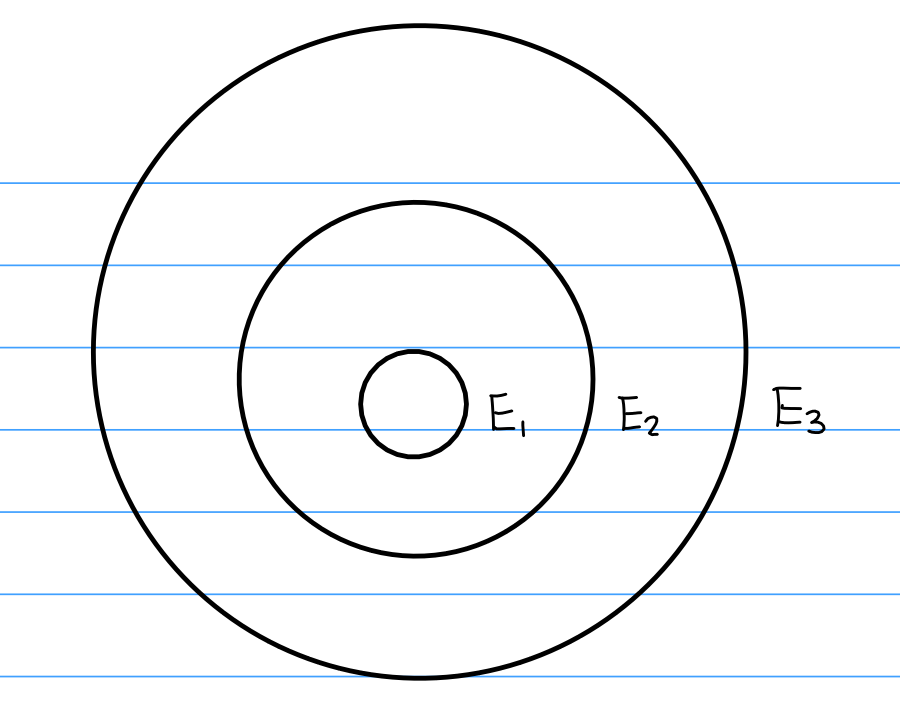
\includegraphics{figures/2019-09-05-11:20.png}\\

Let

\begin{itemize}
\tightlist
\item
  \(A_1 = E_1\)
\item
  \(A_2 = E_2 \setminus E_1\),
\item
  \(\cdots A_j = E_j \setminus E_{j-1}\).
\end{itemize}

Then \(\theset{A_j}\) are disjoint, and \(E = \disjoint A_j\), so

\begin{align*}
m(E) &= \sum_j m(A_j) \\
&= \lim_{k\to\infty} \sum _{j=1}^k \mu (A_j) \\
&= \lim_{k\to\infty} \mu(\union_{j=1}^k A_j) \\
&= \lim_{k\to\infty} \mu (E_k). \quad \qed
\end{align*}

Part (2):

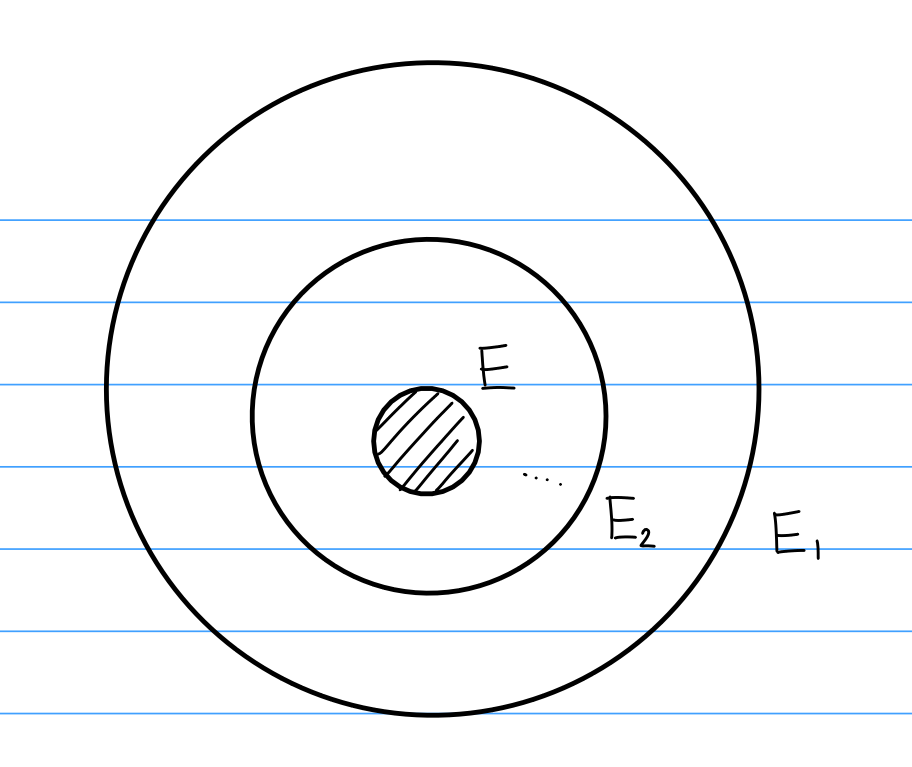
\includegraphics{figures/2019-09-05-11:25.png}\\

Let \(A_i = E_j\setminus E_{j+1}\), so \(\theset{A_i}\) are disjoint.

Then (\textbf{important!!}) \(E_1 = \union A_i \union E\), which are
\textbf{disjoint and measurable}. Then,

\begin{align*}
\mu(E_1) &= \sum \mu(A_i) + \mu(E) \\
&= \lim_{k\to\infty} \sum_{i=1}^{k-1} \mu(A_j) \\
&= \lim_{k\to\infty} \sum_{i=1}^{k-1} \mu(E_i) - \mu(E_{i+1}) + \mu(E),\quad\text{(which is telescoping)} \\
&= \lim_{k\to\infty} (\mu(E_1) - \mu(E_k)) + \mu(E) \\
\implies \mu(E_1) &= \mu(E_1) - \lim_k \mu(E_k) + \mu(E) \quad\text{since } \mu(E_1) < \infty \\
\implies \mu(E) &= \lim_k \mu(E_k) \hfill
.\end{align*}

\(\qed\)

Recall that if \(E\subseteq \RR^n\), then

\begin{align*}
m_*(E) &= \inf\theset{m_*(G) \suchthat E\subset G~\text{open}} \\
&\iff  \\ 
\forall \varepsilon > 0,~~ \exists G \supseteq E &\suchthat m_*(G) \leq m_*(E) + \varepsilon
.\end{align*}

\begin{quote}
Note: this says that the measure is \emph{regular}.
\end{quote}

\hypertarget{approximation-by-compact-sets}{%
\subsection{Approximation by Compact
Sets}\label{approximation-by-compact-sets}}

\textbf{Theorem:} If \(E\subseteq \RR^n\) is measurable, then

\begin{align*}
m(E) = \sup&\theset{m(K) \suchthat K\subseteq E~\text{and $K$ is compact}} \\
\iff & \\
\forall \varepsilon ~\exists ~\text{compact}~ K\subseteq E  \suchthat& m(K) \geq m(E) - \varepsilon
.\end{align*}

\emph{Proof:}

\emph{Case 1:} Suppose \(E\) is bounded.

Let \(\varepsilon > 0\), then by the closed characterization of
measurability, we have \(m(E\setminus F) < \varepsilon\) for some closed
set \(F\subseteq E\).

Since \(E\) is bounded, \(m(E) < \infty\), and so

\begin{align*}
m(E\setminus F) &< \varepsilon  \implies \\
m(E) - m(F) &< \varepsilon \implies \\
m(F) &> m(E) - \varepsilon
.\end{align*}

where since \(F\) is a closed and bounded set in \(\RR^n\), \(F\) is
compact.

\emph{Case 2:} Suppose \(E\) is unbounded. Write
\begin{align*}
E_j = E \intersect_{j=1}^\infty B(j, 0)
,\end{align*} so \(E_j \nearrow E\).

Using continuity from below, we have \(m(E) = \lim_j m(E_j)\).

Suppose \(m(E) < \infty\). Then for some \(j\),
\begin{align*}
m(E_j) \geq m(E) - \varepsilon
.\end{align*}

But \(E_j\) is bounded.

By case 1, there is a compact \(K \subseteq E_j\) where
\begin{align*}
m(K) \geq m(E_j) - \varepsilon
.\end{align*}

But then \(m(K) \geq m(E) - 2\varepsilon\).

Suppose now that \(m(E) = \infty\).

For any \(M > 0\), we can find an \(E_j\) such that
\begin{align*}m(E_j) > M.\end{align*}

Since \(E_j\) is bounded, by case 1 we get a compact
\(K \subseteq E_j \subseteq E\) with \(m(K) > M\).

\(\qed\)

\begin{quote}
Qual alert: very similar arguments are often used on the quals.
\end{quote}

\hypertarget{caratheodory-characterization}{%
\subsection{Caratheodory
Characterization}\label{caratheodory-characterization}}

A subset \(E\subseteq \RR^n\) is measurable iff for all
\(A\subseteq \RR^n\),
\begin{align*}
m_*(A) = m_*(E\intersect A) + m_*(E \intersect A^c).
\end{align*}

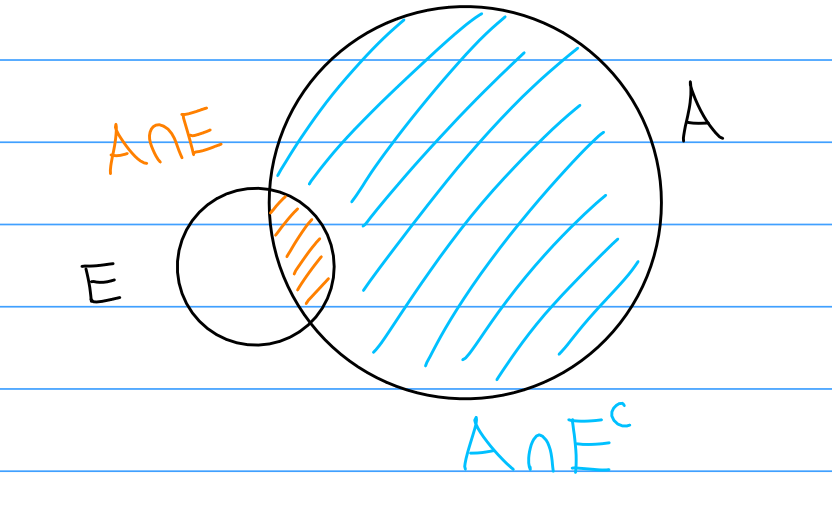
\includegraphics{figures/2019-09-05-12:01.png}\\

Note that this can be interpreted in terms of \emph{inner measures}, in
which we're approximating \(E\) with cubes from the inside. If we also
think of this in terms of probability spaces, we could interpret the RHS
as saying that the probability of an event either happening or
\emph{not} happening should be 1.

\begin{quote}
Note: \(G_\delta\) sets are measurable.
\end{quote}

Note that the \(\leq\) case is satisfied automatically by subadditivity,
and the \(\geq\) case comes from if \(A\subseteq V\) then

\begin{align*}
m(A) \geq \cdots \text{Exercise!}
.\end{align*}

\textbf{Theorem:} Let \(E\subseteq \RR^n\) be measurable. Then

\begin{enumerate}
\def\labelenumi{\arabic{enumi}.}
\item
  For all \(h\in \RR^n\), then \(E+h\) is measurable, and
  \(\mu(E+h) = \mu(E)\).
\item
  For every \(x\in \RR\), the set \(cE\) is measurable and
  \(\mu(cE) = \abs{c}^n \mu(E)\).
\end{enumerate}

We can say more, and determine measures of all linear transformations of
a set in terms of the determinant. Note that because we're working with
cubes in the outer measure, so the only content here is that these new
sets are actually measurable.

If \(E\) is measurable, \(E = H \union Z\) where \(H \in F_\sigma\) and
\(\mu(Z) = 0\). But then \(E+h = (H+h) \union (Z + h)\), but \(H+h\) is
still \(F_\sigma\) because shifts of closed sets are still closed.
Moreover, \(\mu(Z+h) = \mu(Z) = 0\), so were done.

\begin{quote}
Moral: it suffices to check things on Borel sets.
\end{quote}

\hypertarget{thursday-september-12th}{%
\section{Thursday September 12th}\label{thursday-september-12th}}

\hypertarget{measurable-functions}{%
\subsection{Measurable Functions}\label{measurable-functions}}

Let \(E\subseteq \RR^n\) be measurable. Then
\(f: E \to \RR \union \theset{\pm \infty}\) is \emph{Lebesgue
measurable} iff
\begin{align*}
\theset{x \in E \suchthat f(x) > a} = f\inv((a, \infty])) \in \mathcal M
,\end{align*} the collection of Lebesgue measurable sets, for every
\(a\in\RR\).

Similarly, \(E\) is Borel measurable if we replace \(\mathcal M\) by
\(\mathcal B\), the collection of all Borel measurable sets.

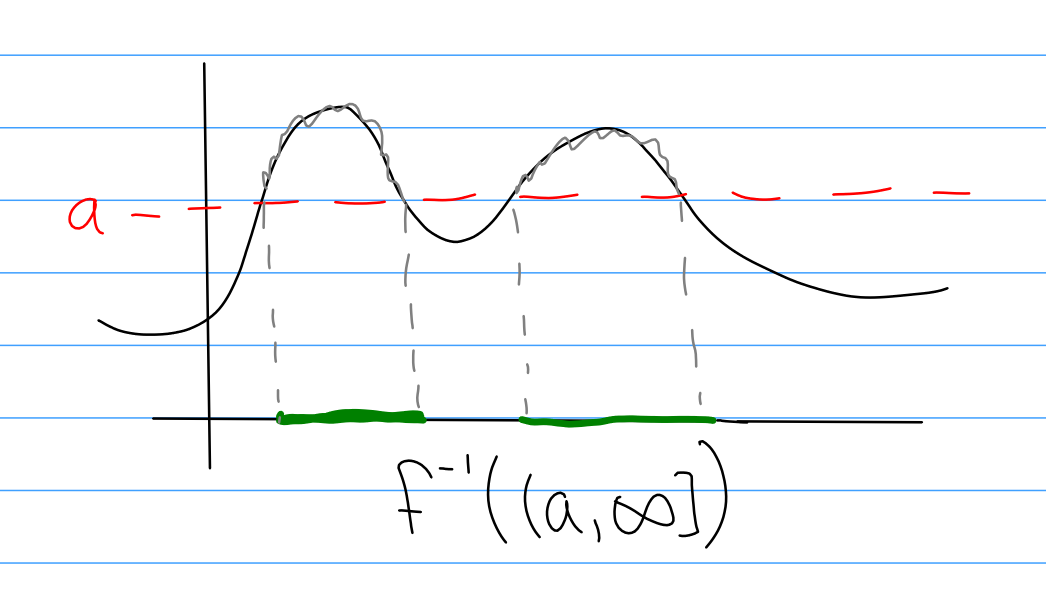
\includegraphics{figures/2019-09-10-11:11.png}\\

As usual, there are many different characterizations:

\begin{itemize}
\tightlist
\item
  \(f\inv((a, \infty])) \in \mathcal M \quad\forall a\in \RR\), since we
  can write this as \(\intersect f\inv((a - \frac 1 k, \infty])\), which
  are all measurable.
\item
  \(f\inv([a, \infty]) \in \mathcal M \quad\forall a\in \RR\), by taking
  complements
\item
  \(f\inv([-\infty, a]) \in \mathcal M \quad\forall a\in \RR\).
\end{itemize}

\textbf{Theorem:} If \(f: E\to \RR\) is finite-valued, then
\begin{align*}
f \text{ is measurable } 
\iff 
f\inv(G) \in \mathcal M \text{ for all open } G\subseteq \RR
.\end{align*}

\emph{Proof:}

\(\impliedby\): Easy, since \((a, \infty)\) is always an open set.

\(\implies\): Suppose \(f\) is measurable and let \(G\subseteq \RR\) be
open, then \(G = \disjoint I_i\) where each \(I_i\) is an interval. Then
\(f\inv(G) = \union f\inv(I_i)\).

But if \(I_i = (a, b)\), then
\(f\inv(I_i)= f\inv((a, \infty)) \intersect f\inv((-\infty, b))\), both
of which are measurable by definition.

\hypertarget{extending-the-class-of-measurable-functions}{%
\subsection{Extending the Class of Measurable
Functions}\label{extending-the-class-of-measurable-functions}}

\textbf{Corollary:} Continuous functions are in fact Borel measurable,
and in particular Lebesgue measurable.

\textbf{Proposition:} If \(f: E\to \RR\) is measurable and
\(\varphi: \RR\to \RR\) is continuous, then \(\varphi \circ f\) is
measurable.

\begin{quote}
Note: This condition can not be relaxed to just \(\varphi\) being
measurable. However, this does work if you require that \(\varphi\) is
Borel measurable.
\end{quote}

\emph{Proof:} Let \(G \subseteq \RR\) be open. Then
\begin{align*}
(\varphi \circ f)\inv (G) = f\inv(\varphi\inv(G)) \in \mathcal M
.\end{align*}

But \(\varphi\inv(G)\) is open since \(\varphi\) is continuous, and thus
measurable, and since \(f\) is a measurable function, this pulls back to
a measurable set, so the composition is measurable.

Consequences of this proposition: If \(f\) is measurable, then so is
\(\abs f, \abs{f}^p, f^2, e^{cf}\), for any constant, etc.

We will show that \(\mathcal M\) is closed under most algebraic and
limiting operations.

\textbf{Theorem 2:} If \(f, g\) are \(\RR\dash\)valued measurable
functions, then \(fg\) and \(f+g\) are measurable.

\begin{quote}
Note that we already know this for \(g\) a constant, since
\(x \mapsto x+c\) and \(x\mapsto cx\) are continuous functions.
\end{quote}

\emph{Proof:} To come later.

An interesting consequence: if \(f,g\) are measurable then
\(\max(f, g)\) is as well, since
\begin{align*}
\max(f, g) = \frac{(f + g) + \abs{f-g}}{2}.
\end{align*} \textbf{Theorem:} If \(\theset{f_n}\) is a sequence of
\(\overline{\RR}\dash\)valued measurable functions, then

\begin{enumerate}
\def\labelenumi{\arabic{enumi}.}
\tightlist
\item
  \(\sup_n f_n\) and \(\inf_n f_n\) are measurable
\item
  \(\limsup_n f_n \definedas \inf_n \sup_{k\geq n} f_k\) is measurable,
  as is the \(\liminf_n f_n\).
\end{enumerate}

\begin{quote}
Note: As a consequence, if \(f_n \to f\) pointwise and each \(f_n\) is
measurable, then \(\limsup f_n = \lim f_n = f\) is measurable.
\end{quote}

\emph{Proof of Theorem 2:}

Suppose \(f,g\) are measurable and finite-valued. Let \(a\in \RR\) and
consider
\begin{align*}
S = \theset{x \suchthat f(x) + g(x) > a }
.\end{align*}

Then
\begin{align*}
S = \theset{ x \suchthat f(x) > -g(x) + a }
,\end{align*} where \(f\) is measurable and so is \(-g + a\).

With the following lemma, we'll be done:

\textbf{Lemma:} If \(f, h\) are measurable, then
\(S = \theset{x \suchthat f(x) > h(x) }\) is always a measurable set.

\emph{Proof:} Since \(f(x) > h(x)\), there is a rational \(q\) such that
\(h(x) < q < f(x)\).

But then
\begin{align*}
S = \union_{q\in\QQ} \theset{x \suchthat f(x) > q > h(x)} = \theset{f > q} \intersect \theset{h < q}
,\end{align*} which is an intersection of measurable sets. \(\qed\)

\begin{quote}
For the set equality, just check that
\(x\in S \implies x \in \union\text{stuff}\), and
\(x\not\in S \implies x \not \in \union \text{stuff}\).
\end{quote}

\begin{quote}
Note: we can write \(fg = \frac{(f+g)^2 - (f-g)^2}{4}\).
\end{quote}

\emph{Proof of Theorem 3:}

Since \(\inf_n f_n(x) = - \sup f_n(x)\), we only need to show that
\(\sup f_n\) is measurable.

For any given \(a\), we want to show that
\(S = \theset{x \suchthat \sup_n f_n(x) > a}\) is measurable.

Then there is some \(n\) for which \(f_n(x) > a\), and the claim is that
\begin{align*}
S = \union_n \theset{x \suchthat f_n(x) > a}
.\end{align*}

But this follows formally by just checking set inclusions. So \(S\) is a
countable union of measurable sets and thus measurable. \(\qed\)

\hypertarget{almost-everywhere-equality}{%
\subsection{Almost Everywhere
Equality}\label{almost-everywhere-equality}}

\textbf{Definition:} If \(f,g: E \to \overline \RR, \CC\) then \(f=g\)
\emph{almost everywhere} (or \(f=g\) a.e.) iff
\begin{align*}
\theset{x \suchthat f(x) \neq g(x)} \text{ is null }
.\end{align*}

\textbf{Fact:} If \(f\) is measurable and \(f=g\) a.e., then \(g\) is
measurable.

This follows because
\begin{align*}
\theset{g > a} = \theset{f > g} \union Z,\end{align*} where
\(Z \subseteq \theset{f\neq g}\), which is null, forcing \(Z\) to be
null as well.

\textbf{Fact:} If \(\theset{f_n}\) is a sequence of measurable functions
and \(f_n \to f\) pointwise a.e., then \(f\) is measurable.

Note that we've replaced open, continuous, uniform etc with a new notion
of ``measurable'' in all instances.

This new notion isn't so far from the original ones, but allows much
more to be done.

\textbf{Littlewood's Principles:}

\begin{itemize}
\item
  Every measurable set is \emph{nearly open} (See \emph{Lebesgue
  density})
\item
  Every measurable function is \emph{nearly continuous} (See
  \emph{Lusin's Theorem})
\item
  Every convergent sequence of measurable functions is \emph{nearly
  uniformly convergent} (See \emph{Egorov's Theorem})
\end{itemize}

\hypertarget{tuesday-september-17th}{%
\section{Tuesday September 17th?}\label{tuesday-september-17th}}

\hypertarget{approximation-by-simple-functions}{%
\subsection{Approximation by Simple
Functions}\label{approximation-by-simple-functions}}

\textbf{Definition:} Let \(E \subseteq \RR^n\) be measurable. Then the
\emph{characteristic function} of \(E\) is defined as

\begin{align*}
\chi_E(x) \definedas 
\begin{cases} 
1 & x \in E \\ 
0 & \text{else.} 
\end{cases}
\end{align*}

\textbf{Definition:} A \emph{step function} is a function of the form
\begin{align*}
S(x) = \sum_{i=1}^N a_i \chi_R(x)
\end{align*} where \(R\) is some rectangle.

\textbf{Definition:} A \emph{simple function} is a function of the form
\begin{align*}
s(x) = \sum_{i=1}^N a_j \chi_{E_j}(x)
\end{align*} where each \(E_j\) is measurable.

\textbf{Theorem 1:} If \(f: E \to [0, \infty]\) is a non-negative
measurable function, then there exists a sequence of simple functions
\(\theset{s_k}\) such that
\begin{align*}
s_k(x) \leq s_{k+1}(x) ~~\forall x, k \quad \text{ and } \quad 
\lim_{k\to\infty} s_k(x) = f(x) ~\forall x
.\end{align*}

\textbf{Corollary:} This in fact holds for \(f: E \to \overline \RR\)
taking on extended real values, not just positive functions.

\emph{Proof:} Write \(f = f^+ - f^-\), where
\(f^+(x) = \max\theset{f(x), 0}\).

\textbf{Theorem 2:} If \(f: E \to \overline \RR\) is measurable, there
exists a sequence \(\psi_k\) of \emph{step} functions such that
\(\psi_k \to f\) almost everywhere.

\emph{Proof:} See homework 3, problem 1c.

\hypertarget{lebesgue-density-theorem}{%
\subsection{Lebesgue Density Theorem}\label{lebesgue-density-theorem}}

\textbf{Theorem (Lebesgue Density):} If \(E\subseteq \RR^n\) is
measurable, then

\begin{align*}
\lim_{r\to 0^+} \frac{m(E \intersect  B(r, x))}{m(B(r, x))} = 1 \quad  \text{for almost every } x \in E. 
\end{align*}

\hypertarget{egorovs-theorem}{%
\subsection{Egorov's Theorem}\label{egorovs-theorem}}

\textbf{Theorem (Egorov):} Let \(E \subseteq \RR^n\) be measurable with
\(m(E) > 0\).

Let \(f_k: E \to \RR\) be a sequence of measurable functions such that
\(f(x) \definedas \lim_{k\to\infty} f_k(x)\) exists a.e. and is finite
valued.

Then the convergence is \emph{almost uniform}, i.e.

\begin{align*}
\forall\varepsilon > 0, ~\exists F \subseteq E ~\text{closed}~ \suchthat & 
m(E\setminus F) < \varepsilon ~\text{and}~ f_k \uniformlyconverges  f ~\text{on}~ F
.\end{align*}

Are these conditions really necessary?

\begin{enumerate}
\def\labelenumi{\arabic{enumi}.}
\item
  If \(E = \RR\), let
  \begin{align*}
  f_k(x)  = \indic{\abs x > k}
  .\end{align*} Then \(f_k \to 0\) a.e. but not ``almost uniformly''.
\item
  If \(E = [0, 1]\), let
  \begin{align*}
  f_k(x) = k\indic{0 \leq x \leq 1 - \frac 1 k}
  .\end{align*} Then
  \begin{align*}
  f_k \to \infty \iff 0 \leq x < 1,~ 0 \iff x = 1,\end{align*} but not
  ``almost uniformly''.
\end{enumerate}

\hypertarget{lusins-theorem}{%
\subsection{Lusin's Theorem}\label{lusins-theorem}}

\textbf{Theorem (Lusin):}

Suppose \(f\) is measurable and finite-valued on a measurable set \(E\)
with \(m(E) < \infty\).

Then \(\forall \varepsilon > 0,~\exists F \subseteq E\) closed such that
\begin{align*}
m(E\setminus F) < \varepsilon 
\text{ and } 
\restrictionof{f}{F} \text{ is continuous }
.\end{align*}

\begin{quote}
This doesn't mean that the original \(f\) is actually continuous on
\(F\), when thought of as a function on \(E\) -- we restrict the
universe to only F, so e.g.~we can only take sequences that are subsets
of \(F\) when we go to check continuity. Example to note:
\begin{align*}
f = \chi_\QQ \intersect [0, 1]
,\end{align*} which is discontinuous at every point.
\end{quote}

\hypertarget{proof-of-egorov}{%
\subsection{Proof of Egorov}\label{proof-of-egorov}}

\emph{Proof of Egorov:} Assume wlog that \(f_k \to f\)
\emph{everywhere}.

\textbf{Lemma:} Let \(E, \theset{f_n}\) and \(f\) be as in Egorov's
theorem.

Then for all \(\varepsilon > 0, \alpha > 0\) there exists a closed set
\(F \subseteq E\) and some \(k_0 \in \NN\) such that

\begin{itemize}
\item
  \(m(E\setminus F) < \varepsilon\), and
\item
  \(\abs{f_k(x) - f(x)} < \alpha\quad \forall x\in F,~ k \geq k_0\).
\end{itemize}

So let \(\varepsilon > 0\), then the lemma tells us that for every \(j\)
we can find a closed set \(F_j \subseteq E\) with
\begin{align*}
m(E\setminus F_j) < \varepsilon / 2^j
\end{align*}

and \(k_j\) such that

\begin{align*}
\abs{f_k(x) - f(x)} < \frac 1 j \text{ on } F_j \quad \forall k \geq k_j
.\end{align*}

So take \(F \definedas \intersect F_j\), which is \emph{closed}.

By subadditivity, we have
\begin{align*}
m(E/F) \leq \sum m(E\setminus F_j) < \varepsilon
\end{align*} by construction.

Note that the convergence is \emph{uniform}, since \(k_j\) in the lemma
already provided the uniform threshold for all points in \(F_j\), and
\(F \subseteq F_j\) for every \(j\). \(\qed\)

\emph{Proof of lemma:} Fix \(\varepsilon, \alpha\).

Define

\begin{align*}
E_j &\definedas \theset{x\in E \suchthat~ \abs{f_k(x) - f(x)} < \alpha~~\forall k > j} \\
&= \intersect_{k=j+1}^\infty \theset{x\in E \suchthat~ \abs{f_k(x) - f(x)} < \alpha}
.\end{align*}

Note \(E_j \subseteq E_{j+1}\) and \(E = \union E_j\), so we have
\(E_j \nearrow E\).

Using continuity from below, \(\lim_j m(E_j) = m(E)\).

Since \(m(E) < \infty\), there exists a \(k_0\) such that
\begin{align*}
j \geq k_0 \implies m(E\setminus E_j) < \varepsilon / 2
.\end{align*}

So choose \(F \subset E_{k_0}\) be closed with the property that
\begin{align*}
m(E_{k_0} \setminus F) \leq \frac \varepsilon  2
.\end{align*}

So if \(x\in F\), then \(x\in E_{k_0}\) and thus \(x\in E_j\) for all
\(j\geq k_0\) since they are nested.

But then
\begin{align*}
k \leq k_0 \implies \abs{f_k(x) - f(x)} < \alpha
,\end{align*} and we're done. \(\qed\)

\hypertarget{convergence-in-measure}{%
\subsection{Convergence in Measure}\label{convergence-in-measure}}

\textbf{Definition:} Let \(E \subseteq \RR^n\) be measurable and
\(f, \theset{f_k}\) be measurable, finite-valued functions defined on
\(E\).

We say that \(f_k \to^m f\) or \(f_k \to f\) \emph{in measure} if for
every \(\alpha > 0\), we have
\begin{align*}
\lim_{k\to\infty} m(\theset{x \in E \suchthat \abs{f_k(x) - f(x)} > \alpha}) = 0
.\end{align*} \(\qed\)

How does this relate to pointwise convergence?

\textbf{Theorem}: If \(m(E) < \infty\), then
\begin{align*}
f_k \to f ~a.e \text{ on } E \iff f_k \to^m f \text{ on } E
.\end{align*}

\emph{Proof:} Exercise using the previous lemma.

\begin{quote}
Note that the converse is false! See homework exercise. There is a
partial converse: convergence in measure will yield a \emph{subsequence}
that converges almost everywhere.
\end{quote}

\hypertarget{thursday-september-19th}{%
\section{Thursday September 19th}\label{thursday-september-19th}}

\hypertarget{review-of-the-lebesgue-integral-for-l}{%
\subsection{\texorpdfstring{Review of the Lebesgue Integral for
\(L^+\)}{Review of the Lebesgue Integral for L\^{}+}}\label{review-of-the-lebesgue-integral-for-l}}

Recall the definition of \(L^+\), and the fact that for any
\(f\in L^+\), there is a sequence \(\theset{f_n}\) of simple functions
in \(L^+\) such that \(f_n \nearrow f\).

Given any simple function \(\phi\), we defined
\begin{align*}
\int \phi = \sum_j a_j m(E_j)
\end{align*} \textbf{iff} this is a standard representation for
\(\phi\).

We then extend to all functions in \(L^+\) by defining
\begin{align*}
\int f \definedas \sup \theset{\int \phi \suchthat 0\leq \phi \leq f,~\phi\text{ simple }}
.\end{align*}

\textbf{Some properties:}

\begin{itemize}
\item
  \(f\leq g \implies \int f \leq \int g\)

  (monotonicity, easy to show)
\item
  \(\int cf = c\int f\)

  (also easy to show)
\item
  \(\int (f + g) = \int f + \int g\)

  (less obvious, follows from MCT)
\end{itemize}

\textbf{Theorem:} If \(\theset{f_n} \subset L^+\), then
\(\sum \int f_k = \int \sum f_k\).

\emph{Proof:} Exercise, not too tricky.

\hypertarget{proof-of-monotone-convergence-theorem}{%
\subsection{Proof of Monotone Convergence
Theorem}\label{proof-of-monotone-convergence-theorem}}

\textbf{Theorem (MCT):} If \(\theset{f_n} \subset L^+\) with
\(f_k \leq f_{k+1}\) and \(f_k \to f\), then
\(\lim \int f_n = \int \lim f_n = \int f\).

\emph{Proof of MCT:} Given any simple \(\phi \in L^+\), define the set
function

\begin{align*}
\mu_\phi: \mathcal M \to [0, \infty] \\
A \mapsto \int_A \phi
.\end{align*}

So if \(\theset{E_k} \subset \mathcal M\) and
\(E_1 \subseteq E_2 \subseteq \cdots\), then
\(\mu_\phi(\union E_k) = \lim \mu_\phi(E_k)\).

\begin{quote}
Note that
\begin{align*}
f_k \in L^+ \implies \lim f_k \in L^+ \quad \text{ and }\quad  f_k \leq f_{k+1} \implies \int f_k \leq \int f_{k+1}
,\end{align*} so the limit on the LHS makes sense.
\end{quote}

Let \(f = \lim f_k\), then
\begin{align*}
\int f_k \leq \int f \text{ for all } k
,\end{align*} so
\begin{align*}
\lim \int f_k \leq \int f.\end{align*}

So we need to show that \(\lim \int f_k \geq \int f\).

Fix \(\alpha \in (0, 1)\) and let \(\phi\) be simple with
\(0 \leq \phi \leq f\). (We'll later show that the result is independent
of this choice.)

Let
\begin{align*}
E_k = \theset{x \suchthat f_k(x) \geq \alpha \phi(x)}
,\end{align*} which we can now say is \emph{clearly} measurable.

Then \(E_1 \subseteq E_2 \subseteq \cdots\) since the \(f_k\) are
increasing. Moreover, \(\union E_k = \RR^n\) (check!), since
\(f_k \to f, \alpha \phi < \phi \leq f\).

Then

\begin{align*}
\int f_g \geq \int_{E_k} 
\geq \alpha \int_{E_k}\phi 
\definedas \alpha \mu_\phi(E_k)
.\end{align*}

But then

\begin{align*}
\lim \int f_k \geq \lim \alpha \mu_\phi(E_k) = \alpha \mu_\phi(\RR^n) = \alpha \int \phi
\quad \forall \alpha, \forall \phi
.\end{align*}

So \(\lim \int f_k \geq \int \phi\) for all \(\phi\) simple with
\(0\leq \phi \leq f\).

Thus
\begin{align*}
\int f = \sup_\phi \int \phi \leq \lim \int f_k
,\end{align*} which is what we wanted to show. \(\qed\)

\hypertarget{chebyshevs-inequality}{%
\subsubsection{Chebyshev's Inequality}\label{chebyshevs-inequality}}

\textbf{Theorem (Chebyshev's Inequality):} If \(f\in L^+\), then
\begin{align*}m(\theset{x \suchthat f(x) \geq \alpha}) \geq \frac 1 \alpha \int f \forall \alpha
.\end{align*}

\emph{Proof:}

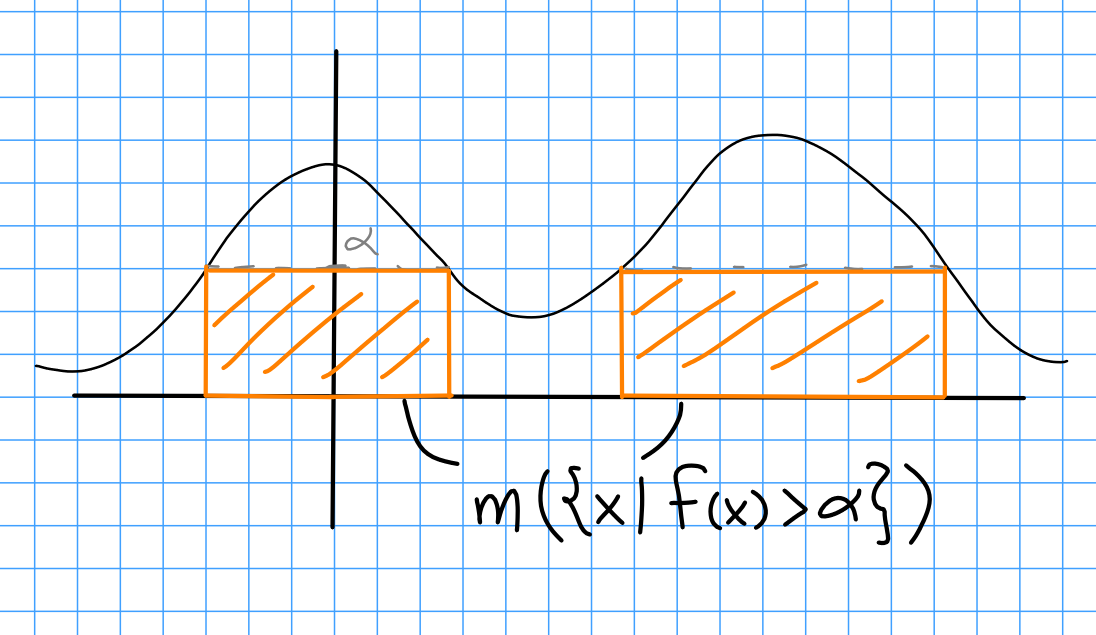
\includegraphics{figures/2019-09-19-11:46.png}\\

Just note that
\begin{align*}
\alpha m(\theset{x \suchthat f(x) > \alpha}) = \int \alpha \chi_{f \geq \alpha} \leq \int f
.\end{align*} \(\qed\)

\hypertarget{the-integral-detects-almost-everywhere-equality}{%
\subsubsection{The Integral Detects Almost-Everywhere
Equality}\label{the-integral-detects-almost-everywhere-equality}}

\textbf{Proposition:} Suppose \(f\in L^+\). Then
\begin{align*}
\int f = 0 \implies f = 0 \text{ a.e. }
\end{align*}

\begin{quote}
Nice trick: showing \(a_n \to L\) can be done by showing
\(a_n - L \to 0\). Similarly,
\begin{align*}
\int f = \int g \iff \int (f-g) = 0 
\end{align*}
\end{quote}

\emph{Proof of Proposition:}

This is obvious for simple functions:

If \(f = \sum a_i \chi_{E_i}\) in standard representation, then
\begin{align*}
\int f = \sum a_j m(E_j) = 0 \iff \text{ either } a_j = 0 ~\forall j, \text{ or } a_j \neq 0 \text{ and } m(E_j) = 0
.\end{align*}

So it only disagrees with zero on a measure zero set.

In general, suppose \(f = 0\) a.e., note that
\begin{align*}
\phi \leq f = 0 \implies \phi = 0 \text{ a.e. }
\end{align*} and thus \(\int \phi = 0\) by the previous case.

But then
\begin{align*}
\int f = \sup_\phi \int \phi = 0 \text{ a.e. }
,\end{align*} and we're done.

Now suppose \(\int f = 0\) a.e.; we can apply Chebyshev,which says that
\begin{align*}
m(\theset{x \suchthat f(x) \geq \alpha}) = 0 
\text{ for any } 
\alpha \geq 0
.\end{align*}

But then \begin{align*}
m(\theset{x \suchthat f(x) > 0}) 
&= m(\union_n \theset{x\suchthat f(x) > \frac 1 n}) \\
&= \lim m(\text{stuff}) \\
&= \lim 0 \\ 
&= 0
.\end{align*}

\(\qed\)

\begin{quote}
\emph{Remark:} In the MCT, the monotonicity is necessary, i.e.~we really
need \(f_k \nearrow f\).
\end{quote}

\emph{Examples:}

\begin{itemize}
\item
  \(f_k = k \chi_{[0, \frac 1 k]}\). Then \(f_k \to 0\) a.e. but
  \(\int f_k = 1\) for all \(k\) while \(\int f = 0\).
\item
  \(f_k = \chi_{[k, k+1]} \to 0\) a.e. (the skateboard to infinity!)
\end{itemize}

\hypertarget{fatous-theorem}{%
\subsection{Fatou's Theorem}\label{fatous-theorem}}

Another convergence theorem, this time with virtually no hypothesis:

\textbf{Theorem (Fatou):} If \(\theset{f_k} \subset L^+\), then
\(\int \liminf f_k \leq \liminf \int f_k\)

\begin{quote}
How to remember: in the above examples, we had \(\int \lim f_k = 0\), so
we can saturate the LHS to zero to obtain an inequality of the form
\(a\leq b\).
\end{quote}

\emph{Proof of Fatou:} We can write
\begin{align*}
\liminf_k f_k = \lim_k g_k \quad \text{ where }\quad  g_k = \inf_{n \geq k} f_n
.\end{align*}

Note that \(g_k \nearrow \liminf_k f_k\), we can apply MCT. So

\begin{align*}
\int \liminf_k f_k 
&= \int \lim_k g_k \\
&=_\text{MCT} \lim_k \int g_k \\
&= \liminf \int g_k \\
&\leq \liminf \int f_k
,\end{align*}

where we can note that
\begin{align*}
g_k \leq f_k \implies \int g_k \leq \int f_k
.\end{align*} \(\qed\)

\hypertarget{dominated-convergence-theorem}{%
\subsection{Dominated Convergence
Theorem}\label{dominated-convergence-theorem}}

\textbf{Theorem (DCT):} If \(\theset{f_k} \subset L^+\), \(f_k \to f\)
a.e., \textbf{and} \(f_k \leq g \in L^+\) where \(\int g < \infty\),
then
\begin{align*}
\int f = \int \lim f_k = \lim \int f_k
.\end{align*}

\hypertarget{tuesday-september-24th}{%
\section{Tuesday September 24th}\label{tuesday-september-24th}}

\hypertarget{convergence-theorems}{%
\subsection{Convergence Theorems}\label{convergence-theorems}}

Two main convergence theorems: define
\(L^+ = \theset{f: \RR^n \to [0, \infty] \suchthat f\text{ is measurable.}}\).
Then

\textbf{Theorem 1 (MCT):} If \(\theset{f_n} \subseteq L^+\) with
\(f_n \nearrow f\), then
\begin{align*}
\int f = \lim \int f_n.\end{align*}

\textbf{Theorem 2 (Fatou's lemma):} If \(\theset{f_n} \subseteq L^+\),
then
\begin{align*}
\int \liminf f_n \leq \liminf \int f_n.
\end{align*}

\textbf{Corollary 1:} If \(\theset{f_n} \subseteq L^+\) and
\(f_n \to f\) a.e. and \(\int f_n \leq M\) uniformly, then
\begin{align*}
\int f \leq M
\end{align*}

\begin{quote}
This uses Fatou's lemma.
\end{quote}

\textbf{Corollary 2:} If \(\theset{f_n} \subseteq L^+\) and
\(f_n \to f\) a.e. with instead \(f_n \leq f\) a.e. for all \(n\), then
\begin{align*}
\int f = \lim \int f_n
.\end{align*}

\emph{Proof:} By Fatou,
\begin{align*}
\int f \leq \liminf \int f_n
.\end{align*}

If we can show \(\limsup \int f_n \leq \int f\) as well, we're done.

Since integrals satisfy monotonicity,
\begin{align*}
f_n \leq f \implies \int f_n \leq \int f ~\text{a.e.}
\end{align*} But by order-limit laws, we then have
\(\limsup \int f_n \leq \int f\) as well. \(\qed\)

\hypertarget{extending-the-integral-to-overline-rrdashvalued-functions-and-cc}{%
\subsection{\texorpdfstring{Extending the Integral to
\(\overline \RR\dash\)valued functions (and
\(\CC\))}{Extending the Integral to \textbackslash overline \textbackslash RR\textbackslash dashvalued functions (and \textbackslash CC)}}\label{extending-the-integral-to-overline-rrdashvalued-functions-and-cc}}

\textbf{Definition:} A function \(f: \RR^n \to \overline \RR\) is
\emph{integrable} iff \(\int \abs f < \infty\). Note that
\(\abs f = f_+ + f_-\), so if \(f:\overline \RR \to \RR\) is integrable,
then
\begin{align*}
\int \abs f = \int (f_+ + f_-) = \int f_+ + \int f_-,
\end{align*} which means both must be finite. We now have two finite
\emph{numbers}, so we can subtract.

\textbf{Definition:} For \(f:\RR^n \to \overline \RR\), we define
\begin{align*}
\int f = \int f_+ - \int f_-.
\end{align*} Similarly, for \(f: \CC \to \overline \RR\), let
\(f = \mathrm{Im} f + i\mathrm{Re} f\), and define
\begin{align*}
\int f = \int \Re f + i\int \Im f.
\end{align*}

\begin{quote}
Note: the space of all \(\overline \RR\) or \(\CC\) valued functions
forms a real (resp. complex) vector space, and the integral is a real
(complex) linear functional. This is not immediate -- multiplying by
scalars is clear, but distributing integrals over sums is not. If
\(h = f + g\), then it is \textbf{not} the case that
\(h_+ = f_+ + g_+\). But we can write out
\begin{align*}
h = f + g \implies h_+ + h_- = f_+ + f_- + g_+ + g_-
,\end{align*} maneuver things so that everything is positive, and
\emph{then} take integrals.
\end{quote}

\hypertarget{l1-and-its-norm}{%
\subsection{\texorpdfstring{\(L^1\) and its
Norm}{L\^{}1 and its Norm}}\label{l1-and-its-norm}}

\textbf{Definition}: We can provisionally define
\begin{align*}
L^1 = \theset{f: \RR^n \to \CC: f\text{ is measurable }},
\end{align*}

where we'd like to define
\begin{align*}
\norm{f}_{L^1} \definedas \int \abs f
.\end{align*}

However, this only yields a \emph{seminorm}, since nonzero functions
still end up with zero norm. This can be remedied by identifying
functions which agree on a set of measure zero.

\textbf{Proposition (Triangle Inequality for \(L^1\) Seminorm):} If
\(f\in L^1\), then \(\abs{\int f} \leq \int \abs f\).

\emph{Proof:} This is trivial if \(\int f = 0\). If \(f\) is
\(\RR\dash\)valued, then

\begin{align*}
\abs{\int f} 
&= \abs{\int f_+ - \int f_-} \\
&\leq \abs{\int f_+} + \abs{\int f_-} \\
&= \int f_+ + \int f_- \\
&= \int f_+ + f_- \\
&= \int \abs{f}
.\end{align*}

If \(f\) is \(\CC\dash\)valued, then \(\abs z = \frac{z^* z}{\abs z}\),
so

\begin{align*}
\frac{(\int f)^*}{\abs{\int f}} \int f 
&\definedas \alpha \int f \\
&= \int \alpha f \\
&= \int \mathrm{Re}(\alpha f) + i\int\mathrm{Im}(\alpha f) 
.\end{align*}

but since what we started with was \emph{real}, the imaginary component
vanishes, so this equals
\begin{align*}
\int \mathrm{Re}(\alpha f) = \abs{\int \mathrm{Re}(\alpha f) } \leq \int \abs{\mathrm{Re}(\alpha f) } \leq \int \abs{\alpha f} = \int \abs{f}.
\end{align*}

\begin{quote}
Note: this is referred to as a \textbf{rotation/triangle trick}.
\end{quote}

\textbf{Actual definition of \(L^1\):} Let \(X \subseteq \RR^n\) be
measurable. Then
\begin{align*}
L^1(X) = \theset{\text{equivalence classes of a.e. defined integrable functions on $X$}}
\end{align*}

This is an equivalence relation, and we write \(f\sim g \iff f = g\)
a.e.

We then define \(\norm{f}_1 = \int_X \abs f\).

We have
\begin{align*}
\int \abs f = 0 ~\text{a.e.} \iff f = 0 ~\text{a.e.}
\end{align*}

\emph{Exercise}: Prove this for \(L^+\) functions.

We'd like this to also be true iff \(\int_E f = 0\) for all measurable
\(E \subseteq X\).

\hypertarget{dominated-convergence-theorem}{%
\subsection{Dominated Convergence
Theorem}\label{dominated-convergence-theorem}}

The following theorem will apply whenever we want to switch integrals
and limits, but \(f\) is \emph{not necessarily} in \(L^+\).

\begin{quote}
This is the ONLY theorem that doesn't require non-negativity!!!
\end{quote}

\textbf{Theorem (DCT):} Suppose \(\theset{f_n} \in L^1\), \(f_n \to f\)
a.e., and \(\abs{f_n} \leq g\) a.e. for all \(n\) with \(g\in L^1\).

Then \(f\in L^1\) and
\begin{align*}
\int f = \lim \int f_n \quad\text{and}\quad \lim \int\abs{f_n - f} = 0
\end{align*}

\begin{quote}
Note that the second statement is stronger, and in fact implies the
first. This statement is what we'll prove.
\end{quote}

\emph{Proof:} Since \(f_n \to f\) and each \(f_n\) is measurable, then
\(f\) is measurable. Since \(f_n \leq g\) for all \(n\), then
\(f \leq g\). So
\begin{align*}\int \abs{f} \leq \int \abs{g} < \infty
,\end{align*} and thus \(f\in L^1\).

It suffices to show that \(\limsup \int \abs{f_n - f} \leq 0\).

We have to get something non-negative to apply anything we know so far,
so

\begin{align*}
0 \leq \abs{f_n - f} \leq \abs {f_n} + \abs f \leq g + \abs f \\
\implies g + \abs f - \abs{f_n - f} \geq 0 \\
(\text{This is where we'll apply Fatou.}) \\
\implies \int \liminf (g + \abs f - \abs{f_n -f}) &\leq \liminf \int (g + \abs f - \abs{f_n - f})\\
\implies \int (g + \abs f) &\leq \liminf \int(g + \abs f) - \liminf \int\abs{f_n - f} \\
\implies \int (g + \abs f) &\leq \int(g + \abs f) + \limsup \int\abs{f_n - f} \\
\implies 0 &\leq \limsup \int\abs{f_n - f}. \qed
\end{align*}

\(\qed\)

\hypertarget{differentiating-under-the-integral}{%
\subsection{Differentiating Under the
Integral}\label{differentiating-under-the-integral}}

Let
\begin{align*}
F(t) = \int f(x, t)~dx
\end{align*}

\begin{itemize}
\tightlist
\item
  Is \(F\) continuous at a point \(t_0\)?
\item
  Is \(F\) differentiable at \(t_0\)?
\end{itemize}

We could show continuity by looking at

\begin{align*}
\lim_{t \to t_0} \abs{F(t) - F(t_0)} 
\leq \lim_{t\to t_0} \int \abs{f(x, t) - f(x, t_0)} 
\leq_{DCT} \int \lim \abs{f(x, t) - f(x, t_0)}
.\end{align*}

which will go to zero exactly when \(f\) is continuous in \(t\).

Differentiability can be shown by considering

\begin{align*}
\lim \frac{\abs{F(t_0) - F(t)}}{t - t_0}
&\leq \lim \int \frac{f(x, t) - f(x, t_0)}{t - t_0} ~dx \\
&\leq \int \lim \frac{f(x, t) - f(x, t_0)}{t - t_0}~dx \\
&= \int f'(x, t_0)~dx
.\end{align*}

\hypertarget{thursday-september-26th}{%
\section{Thursday September 26th}\label{thursday-september-26th}}

\hypertarget{l1-and-its-convergence-theorems}{%
\subsection{\texorpdfstring{\(L^1\) and its Convergence
Theorems}{L\^{}1 and its Convergence Theorems}}\label{l1-and-its-convergence-theorems}}

For any measurable \(X \subseteq \RR^n\), we defined
\begin{align*}
L^1(X) = \theset{f: X \to \CC \text{ measurable } \suchthat \int_X \abs f < \infty}/ \sim
\end{align*} where \(f\sim g \iff f = g\) a.e.

\begin{quote}
Note that we could talk about \(\overline \RR\) valued functions,
\emph{but} (theorem) integrable functions can only be finite on a null
set. So we can stop considering these altogether if we're just
considering \(L^1\) functions.
\end{quote}

The space \(L^1\) is in fact a \emph{normed vector space} with
\begin{align*}
\norm{f}_{L^1(X)} \definedas \int_X \abs f
.\end{align*}

\begin{quote}
Recall that we needed to identify functions because this was only a
\emph{seminorm} otherwise, and we only want the zero function to have
norm zero.
\end{quote}

We say
\begin{align*}
f_n \mapsvia{L^1} f \iff \norm{f_n - f}_1 \to 0
.\end{align*}

\textbf{Convergence Theorems:}

\begin{quote}
Mantra: Everything positive and some positivity: MCT. More often: DCT.
\end{quote}

\begin{itemize}
\item
  \textbf{MCT}:
  \begin{align*}
  f_n \in L^+, \quad f_n \nearrow f \text{ a.e. } \implies \lim \int f_n = \int f
  .\end{align*}

  \begin{itemize}
  \item
    Note that it's very important that \(f_n \in L^+\)
  \item
    \textbf{Corollary}:
    \begin{align*}
    \sum \int f_n = \int \sum f_n
    .\end{align*}
  \end{itemize}
\item
  \textbf{DCT:}
  \begin{align*}
  f_n \in L^1,\quad f_n \to f \text{ a.e. },\quad \abs f_n \leq g \in L^1 \implies \lim \int f_n = \int f
  .\end{align*}

  \begin{itemize}
  \tightlist
  \item
    \textbf{A Stronger statement}:
    \begin{align*}
    f_n \mapsvia{L^1} f \quad \text{ i.e. } \int \abs{f_n - f} \to 0
    .\end{align*} The previous statement only gives
    \(\abs{\int f_n - f} \to 0\). This follows because
    \begin{align*}
    \lim \int \abs{f_n - f} =_{DCT} \int \lim \abs{f_n - f} \to 0
    ,\end{align*} since \(\abs{f_n - f} \leq 2g\).
  \end{itemize}
\end{itemize}

\hypertarget{commuting-sums-with-integrals}{%
\subsection{Commuting Sums with
Integrals}\label{commuting-sums-with-integrals}}

\textbf{Theorem:} If

\begin{itemize}
\tightlist
\item
  \(f_n \in L^1\), and
\item
  \(\sum_n \int \abs f_n < \infty\),
\end{itemize}

Then \(\sum_n f_n\) converges to an \(L^1\) function and
\begin{align*}
\sum_n \int f_n = \int \sum f_n
.\end{align*}

\begin{quote}
Note that uniform convergences \(\implies\) pointwise \(\implies\) a.e.
convergence, and so we should think of convergence in norm as
\emph{weaker} than all of these (although they are not actually
comparable).
\end{quote}

\emph{Proof:} By the MCT, we know
\begin{align*}
\int \sum \abs f_n =_{MCT} = \sum \int \abs f_n
,\end{align*} which is integrable, and so the first term is integrable
as well.

By the homework problem,
\begin{align*}
\sum \abs f_n \in L^1 \implies \sum \abs{f_n(x)} < \infty \text{ for almost every } x
.\end{align*} So consider just these \(x\) values.

\begin{quote}
Note that ``\(\RR\) is complete'' is equivalent to ``absolutely
convergent implies convergent'' for sums.
\end{quote}

So for each \(x\), \(\sum f_n(x)\) converges. What are the partial sums?
\begin{align*}
\abs{\sum^N f_j(x)} \leq \sum^\infty \abs{f_j(x)} \quad \forall j,~~a.e.~x.
\end{align*}

So let \(g_N = \sum^N f_j\), so \(g_N\) is dominated by
\(g \definedas g_\infty\). Then

\begin{align*}
\int \sum_j^\infty f_j 
&= \int \lim_{n\to\infty} \sum_{j=1}^n f_j \\
&=_{DCT} \lim_{n\to\infty} \sum_{j=1}^n \int f_j \\
&= \sum_{j=1}^\infty \int f_j
.\end{align*}

\(\qed\)

\begin{quote}
Note that these partial sums are converging a.e., \textbf{and in
\(L^1\)}. We didn't use this here, but it will be important when we want
to show that \(L^1\) is complete.
\end{quote}

\hypertarget{different-notions-of-convergence}{%
\subsection{Different Notions of
Convergence}\label{different-notions-of-convergence}}

Note that \(f_n \to f\) can mean many things:

\begin{enumerate}
\def\labelenumi{\arabic{enumi}.}
\tightlist
\item
  Uniform:
  \(f_n \uniformlyconverges f: \forall \varepsilon ~\exists N \suchthat ~n\geq N \implies \abs{f_N(x) - f(x)} < \varepsilon \quad \forall x.\)
\item
  Pointwise: \(f_n(x) \to f(x)\) for all \(x\). (This is just a sequence
  of numbers)
\item
  Almost Everywhere: \(f_n(x) \to f(x)\) for almost all \(x\).
\item
  Norm: \(\norm{f_n - f}_1 = \int \abs{f_n(x) - f(x)} \to 0\).
\end{enumerate}

We have \(1 \implies 2 \implies 3\), and in general no implication can
be reversed, but (\textbf{warning}) none of \(1,2,3\) imply \(4\) or
vice versa.

\textbf{Examples}:

\begin{itemize}
\item
  \(f_n = n\inv \chi_{[0, n]}\). This converges uniformly to 0, but the
  integral is identically 1. So this satisfies 1,2,3 and not 4.

  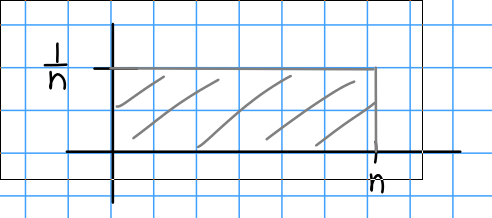
\includegraphics{figures/2019-09-29-19:09.png}\\
\item
  \(f_n = \chi_{(n, n+1)}\) (skateboard to infinity). This satisfies 2,3
  but not 1, 4.
\item
  \(f_n = n\chi_{(0, \frac 1 n)}\). This satisfies 3 but not 1,2,4.
\item
  \(f_n:\) see weird example below. Then \(f_n \to 0\) in \(L^1\) but is
  not 1,2, or 3.

  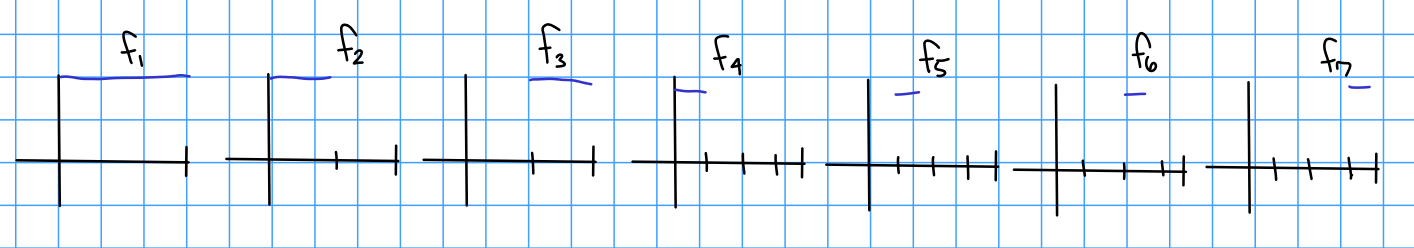
\includegraphics{figures/2019-09-29-19:08.png}\\
\end{itemize}

\hypertarget{comparing-l1-convergence-to-a.e.-convergence}{%
\subsection{\texorpdfstring{Comparing \(L^1\) Convergence to a.e.
Convergence}{Comparing L\^{}1 Convergence to a.e. Convergence}}\label{comparing-l1-convergence-to-a.e.-convergence}}

\textbf{Theorem:} If \(f_n \to f \in L^1\), then there is a subsequence
\(f_{n_k}\) such that \(f_{n_k} \to f\) almost everywhere.

\begin{quote}
Note: convergence always implies Cauchy, so we'll assume this right
away.
\end{quote}

Since \(f_n\) converges in \(L^1\), it is Cauchy in \(L^1\), so
\(\norm{f_n - f_m}_1 \to 0\).

\begin{quote}
Note: we want to pick a sequence that is converging \emph{faster} when
we construct our subsequence, since that's the obstruction to a.e.
convergence.
\end{quote}

So there is a subsequence \(n_1, n_2, \cdots\) such that
\(\norm{f_n - f_m} \leq 2^{-k}\) if \(n, m \geq n_k\). Let
\(g_1 = f_{n_2}, g_k = f_{n_{k+1}} - f_{n_k}\) be the consecutive
differences. Then

\begin{itemize}
\tightlist
\item
  \(\norm{g_{k+1}} \leq 2^{-k}\) for all \(k\),
\item
  \(f_{n_k} = \sum_{j=1}^{k} g_j\)
\end{itemize}

Thus we want to show that this sum converges almost everywhere to an
\(L^1\) function. So if \(\sum_{j=1}^\infty \norm{g_j}_1 < \infty\),
we're done.

We have
\begin{align*}
\sum \norm{g_j} = \norm{g_1} + \sum_j 2^{-j}
.\end{align*} By the previous theorem, this means
\(f_{n_k} = \sum^k g_j \mapsvia{a.e.} f\).

We know it converges to \emph{some} \(L^1\) function, \textbf{but limits
are unique}, so this is actually the original \(f\). \(\qed\)

\hypertarget{completeness-of-l1}{%
\subsection{\texorpdfstring{Completeness of
\(L^1\)}{Completeness of L\^{}1}}\label{completeness-of-l1}}

\textbf{Theorem:} \(L^1\) is a complete normed space, i.e.~\textbf{a
Banach space}, so every Cauchy sequence in \(L^1\) converges to a
function in \(L^1\).

\emph{Proof:}

\begin{quote}
Proofs of completeness tend to go the same way:
\end{quote}

\begin{quote}
\begin{enumerate}
\def\labelenumi{\arabic{enumi}.}
\tightlist
\item
  Take a Cauchy sequence \(\theset{f_n}\).
\item
  Find a candidate limit \(f\)
\item
  Show that the \(f_n\) actually converge to this candidate \(f\)
\item
  Show that \(f\) is in \(L^1\).
\end{enumerate}
\end{quote}

So suppose \(f_n\) is Cauchy.

From the previous theorem, we know a subsequence (all in \(L^1\))
converges to some limit \(f\) in \(L^1\). So let this \(f\) be the
candidate limit, we just need to show that \(\norm{f_n - f}_1 \to 0\).

Let \(\varepsilon > 0\) and choose \(k\) large enough such that

\begin{itemize}
\tightlist
\item
  \(2^{-k} \leq \frac 1 2 \varepsilon\).
\item
  \(\norm{f_{n_k} - f}_1 \leq \varepsilon\).
\end{itemize}

Then \begin{align*}
\norm{f_n - f}_1 
&\leq \norm{f_n - f_{n_k}}_1 + \norm{f_{n_k} - f}_1 \\
&\leq 2^{-k} + \varepsilon/2 \\
&\leq \varepsilon/2 + \varepsilon/2 = \varepsilon
.\end{align*}

\(\qed\)

\hypertarget{tuesday-october-1}{%
\section{Tuesday October 1}\label{tuesday-october-1}}

\hypertarget{completeness-of-l1-revisited}{%
\subsection{\texorpdfstring{Completeness of \(L^1\)
(Revisited)}{Completeness of L\^{}1 (Revisited)}}\label{completeness-of-l1-revisited}}

\textbf{Last time:} \(L^1\) is complete, where we used the fact that
\(\RR\) is complete in the following way

\textbf{Theorem:} \begin{align*}
\RR \text{ is complete } \iff \left( \sum \abs x_n \infty \implies \sum x_n < \infty \right)
.\end{align*}

\emph{Proof:}

\(\implies\):\\
Suppose \(\RR\) is complete and \(\sum \abs x_n < \infty\).

Let \(S_N = \sum_{i=1}^N x_n\). Then if \(N > M\),
\begin{align*}
\abs{S_N - S_M} \leq \sum_{i=M+1}^N \abs x_n \to 0
.\end{align*}

\(\impliedby\): Suppose every absolutely convergent series is
convergent.

Let \(\theset{x_n}\) be Cauchy; we want to show that it is convergent as
well.

\begin{quote}
Note: we'll use the same trick as last time. The goal is to cook up an
absolutely convergent sequence, the convergence of which will imply
convergence of our original series.
\end{quote}

Choose a subsequence
\begin{align*}
n_1 \leq n_2 \leq \cdots \quad \text{ such that }\quad  \abs{x_n - x_m} < 2^{-j} \quad \text{ if }\quad  n, m \geq n_j
.\end{align*}

Let \(y_1 = x_{n_1}\) and \(y_j = x_{n_j} - x_{n_{j-1}}\) for \(j > 1\).

Then
\begin{align*}
x_{n_k} = \sum_{i=1}^k y_j \quad \text{and} \quad \sum_{j=1}^\infty \abs{y_j} \leq \abs y_1 + \sum_{j=2}^\infty 2^{-k} < \infty.
\end{align*}

So \(\lim x_{n_k}\) exists and equals \(\sum y_j\).

It follows that for \(n > n_k\) and \(k\) is sufficiently large,
\begin{align*}
\abs{x_n - x} \leq \abs{x_n - x_{n_k}} + \abs{x_{n_k} - x} < \varepsilon
.\end{align*}

\(\qed\)

\textbf{Theorem (Modified):} Let \(X\) be a normed vector space.

\begin{align*}
X \text{ is complete } \iff \left( \sum_n \norm {x_n} < \infty \implies \sum_n x_n < \infty \right)
.\end{align*}

\emph{Proof:} Completely the same, just replace absolute values with
norms everywhere!

\hypertarget{translation-and-dilation-invariance-of-the-lebesgue-integral}{%
\subsection{Translation and Dilation Invariance of the Lebesgue
Integral}\label{translation-and-dilation-invariance-of-the-lebesgue-integral}}

\begin{quote}
Qual Problem Alert!
\end{quote}

\textbf{Definition}: Define a \emph{translation}
\(\tau_h(x) \definedas x+h\) and \(\tau f(x) \definedas f(x-h)\) for all
\(h\in\RR\units\).

\textbf{Definition:} Define a \emph{dilation}
\(f_\delta(x) \definedas \delta^{-n} f(\delta\inv x)\) for all
\(\delta > 0\).

\textbf{Theorem:}

\begin{enumerate}
\def\labelenumi{\arabic{enumi}.}
\item
  \begin{align*}
  f\in L^1 \implies \tau_h f\in L^1 &\text{ and } \int \tau_h f = \int f \\ 
  &\left( \text{i.e. } \int_E f(x-h) = \int_{E + h} f \right)
  .\end{align*}
\item
  \begin{align*}
  f\in L^1 \implies f_\delta \in L^1 &\text{ and } \int f_\delta = \int f \\ 
  &\left( \text{i.e. } \delta^{-n} \int f(\delta\inv x) = \int f(y) \right)
  .\end{align*}
\end{enumerate}

\emph{Proof:} We first verify this for \(f = \chi_E\) where
\(E \in \mathcal M\).

We have \(\tau_h f(x) = f(x-h) = \chi_E(x-h) = \chi_{E + h}(x)\) and
\begin{align*}
\int \tau_n f = m(E+h) = m(E) = \int f
,\end{align*} where we know the measures are equal by translation
invariance of measure.

By linearity, this holds for simple functions as well.

\begin{quote}
Useful technique: once you know something for simple functions, you can
often apply MCT to get it for \(L^+\) functions as well!
\end{quote}

If now \(f\in L^+\) then there exists a sequence of simple functions
\(\theset{\phi_k} \nearrow f\), and by the MCT,
\begin{align*}
\int \phi_k \to \int f
.\end{align*}

Note that
\begin{align*}
\theset{\tau_h \phi_k} \nearrow \tau_h f
,\end{align*} so
\begin{align*}
\int \tau_h \phi_k \to \int \tau_h f
.\end{align*}

But \(\theset{\int\tau_h \phi_k} = \theset{\int\phi_k}\), so \textbf{by
uniqueness of limits} we must have
\begin{align*}
\int f = \int \tau_h f
.\end{align*}

Now this follow for \(\RR\dash\)valued functions by writing
\(f = f_+ - f_-\), and then for \(\CC\dash\)valued functions by
\(f = \Re(f) + i \Im(f)\).

\(\qed\)

\hypertarget{agreement-of-riemann-and-lebesgue-integrals}{%
\subsection{Agreement of Riemann and Lebesgue
Integrals}\label{agreement-of-riemann-and-lebesgue-integrals}}

\textbf{Theorem:} Let \(f\) be a bounded \(\RR\dash\)valued function on
a closed interval \([a,b]\).

If \(f\) is Riemann integrable, then \(f \in L^1\) (so
\(\mathcal{R} \subseteq L^1\) is a subspace) and the integrals agree, so
\begin{align*}
\int_a^b f(x)~dx = \int_{[a,b]} f(x)~dx
\end{align*}

\emph{Proof:} Given a partition \(P = \theset{t_1, t_2, \cdots t_n}\) of
\([a,b]\), let

\begin{align*}
G_p &= \sum_{j=1}^n \sup \theset{f(x) \suchthat x \in [t_k, t_{j+1}]} \chi_{[t_j, t_{j+1}]} \\
g_p &= \sum_{j=1}^n \inf \theset{f(x) \suchthat x \in [t_k, t_{j+1}]} \chi_{[t_j, t_{j+1}]}
.\end{align*}

Then \(\int G_p = U(f, P)\) and \(\int g_p = L(f, p)\) where \(U, L\)
denote the upper and lower sums. Note that the Riemann integral is the
infimum of the former and the supremum of the latter, over increasingly
fine partitions.

So let \(\theset{P_k}\) be a sequence of partitions with the size of the
mesh going to 0.

Then \(G_{P_k} \searrow G\) is converging to something, and
\(g_{p_k} \nearrow g\). In particular, we have
\begin{align*}
G_P \leq f \leq g_P \quad \text{ and so }\quad G \leq f \leq g
.\end{align*}

Since \(f\) is bounded, say by \(M\), then both of these sequences are
dominated by \(\pm M \chi_{[a, b]} \in L^1\).

So we can invoke the DCT, which yields
\begin{align*}
\int G_{P_k} \to \int G \text{ and } \int g_{P_k} \to \int g
,\end{align*} and thus
\begin{align*}
\int g = \int G = \int_\mathcal{R} f
.\end{align*}

Since
\begin{align*}
\int G = \int g \implies \int (G-g) = 0 \implies G = g \text{ a.e. }
,\end{align*} we have \(f = G\) a.e.

But \(G\) is a sequence of measurable function, and so \(f\) is
measurable. Moreover, \(\int G = \int f\). But
\(\int G = \int_\mathcal{R} f\) as well, so the two integrals agree.

\begin{quote}
Recall that
\begin{align*}
f = 0 \text{ a.e. } \iff \int_E f = 0 \text{ for all } E \subseteq \mathcal{M}
.\end{align*}
\end{quote}

\(\qed\)

Examples next time:

Continuous functions with compact support are dense in \(L^1\), which is
a version of the following:

\textbf{Littlewood's Principle}: Any integrable function is \emph{almost
} continuous, in the sense that for any \(f\) and any \(\varepsilon >0\)
there is a continuous function \(g\) such that
\begin{align*}
\int f - \int g < \varepsilon
.\end{align*}

\hypertarget{thursday-october-3}{%
\section{Thursday October 3}\label{thursday-october-3}}

\hypertarget{relating-zero-functions-to-zero-integrals-over-measurable-sets}{%
\subsection{Relating Zero Functions to Zero Integrals Over Measurable
Sets}\label{relating-zero-functions-to-zero-integrals-over-measurable-sets}}

\textbf{Theorem:} \(f = 0\) a.e. iff \(\int_E f = 0\) for all
\(E\in\mathcal{M}\).

If \(f \in L^+\) we already know that \(f=0\) a.e. iff \(\int f = 0\).

\(\implies\): Since \(f = 0\) a.e., we have \(\abs f = 0\) a.e. and
since \(\abs{f} \in L^+\) we have \(\int \abs{f} = 0\).

Now let \(E \in \mathcal{M}\); then

\begin{align*}
\abs{\int_E f} \leq \int_E \abs{f} \leq \int \abs{f} = 0
.\end{align*}

\(\impliedby\): Suppose \(\int_E f = 0 ~~\forall E \in \mathcal{M}\) and
\(f\neq 0\) a.e., then either

\begin{enumerate}
\def\labelenumi{\arabic{enumi}.}
\item
  \(f+\) is positive on a set of nonzero measure, or
\item
  \(f^-\) is positive on a set of nonzero measure.
\end{enumerate}

So suppose wlog (1) holds.

Let \(E = \theset{x \suchthat f^+ > 0}\), then \(m(E) > 0\).

Then \(\int_E f^+ > 0\), since \(\chi_E f^+ \neq 0\) almost everywhere.

We also know that \(f^+ \in L^+\), so
\begin{align*}
f^+ = 0 \text{ a.e. } \iff \int f = 0
.\end{align*} But then \(\int _E f > 0\), since
\begin{align*}
\mathrm{support}(f^+) \intersect \mathrm{support}(f^-) = \theset{x \suchthat f(x) = 0}
,\end{align*} so \(f^- = 0\) on \(E\).

\(\qed\)

\hypertarget{approximation-theorems-and-dense-subspaces-of-l1}{%
\subsection{\texorpdfstring{Approximation Theorems and Dense Subspaces
of
\(L^1\)}{Approximation Theorems and Dense Subspaces of L\^{}1}}\label{approximation-theorems-and-dense-subspaces-of-l1}}

\textbf{Definition:} We say that a collection \(\mathcal{C}\) of
functions is \emph{dense} in \(L^1\) iff
\begin{align*}
\forall\varepsilon>0 ~\text{ and }~ \forall f\in L^1,
\quad \exists g\in\mathcal{C} 
\quad \text{such that} \quad \norm{f-g}_1 < \varepsilon.
\end{align*}

\textbf{Theorem(s):}

\begin{enumerate}
\def\labelenumi{\arabic{enumi}.}
\item
  Simple functions are dense in \(L^1\). \textbf{(DCT)}
\item
  Continuous functions with compact support (\(C_c\) or \(C_0\)) are
  dense in \(L^1\).
\item
  Step functions are dense in \(L^1\).
\end{enumerate}

\emph{Proof of (1):} Let \(f\in L^1\) and \(\varepsilon > 0\).

Since \(f\) is measurable, there exists a sequence of simple functions
\(\theset{\phi_k} \to f\) pointwise with
\(\abs{\phi_k} \leq \abs{\phi_{k+1}}\). Then \(f\) dominates \(\phi_k\)
and the DCT yields \(\int\abs{\phi_k - f} < \varepsilon\) for \(k\)
large enough.

\(\qed\)

\begin{quote}
We'll use this as a stepping stone -- we really want to get
\emph{continuous functions}, but now we can show there are continuous
functions arbitrarily close to \emph{simple} functions, and the triangle
inequality will give us the desired result.
\end{quote}

\emph{Proof of (2):} We have shown that there exists a simple function
\(\phi = \sum_{j=1}^N a_j \chi_{E_j}\) in standard representation, where
\(a_j \neq 0\) and the \(E_j\) are disjoint, with
\(\int \abs{f - \phi} < \varepsilon\).

It suffices to show that for all \(j\), there exists a \(g_j \in C_c\)
such that \(\norm{\chi_{E_j} - g_j} < \varepsilon\).

Note that if we have this, we can define \(g = \sum a_j g_j \in C_c\).

But then

\begin{align*}
\int\abs{\phi - g} = \int \abs{\sum_i^N a_i (\chi_{E_j} - g_j) } \leq \sum_i^N \abs{a_i} \abs{\chi_{E_j} - g_j} \leq C\varepsilon
.\end{align*}

Then applying the triangle inequality yields the desired result.

\textbf{Important Observation:}

Each \(E_j\) has finite measure, so we have
\begin{align*}
m(E_j) = \frac{1}{\abs{a_j}} \int_{E_j} \abs{\phi} \leq \frac{1}{\abs{a_j}}\int \abs{\phi} < \infty
.\end{align*}

\textbf{Claim:} If \(m(E) < \infty\), then there exists a \(g\in C_c\)
such that \(\norm{\chi_E - g}_1 < \varepsilon\) for any
\(\varepsilon > 0\).

\emph{Proof:} Note that we can find a \(K \subseteq E \subseteq G\) such
that \(K\) is compact, \(G\) is open, and
\(m(G\setminus K) < \varepsilon\).

Since \(K\) is closed and \(G^c\) is closed, \textbf{by Urysohn's
Lemma}, there is a continuous \(g\) such that
\(\chi_K \leq g \leq \chi_G\). But then \(g\) is zero on \(G^c\) and 1
on \(K\).

Then \(\abs{\chi_E - g}\) is supported on \(G\setminus K\), so
\begin{align*}
\int\abs{\chi_E - g} \leq m(G\setminus K) < \varepsilon
.\end{align*} \(\qed\)

\begin{quote}
Remark: We will eventually show that \emph{smooth} compactly supported
functions are also dense in \(L^1\).
\end{quote}

This approximation theorem yields some nice proofs:

\hypertarget{small-tails-and-absolute-continuity}{%
\subsection{Small Tails and Absolute
Continuity}\label{small-tails-and-absolute-continuity}}

\textbf{Proposition:} If \(f\in L^1\) and \(\varepsilon > 0\), then

\begin{enumerate}
\def\labelenumi{\arabic{enumi}.}
\item
  \textbf{Small tails}:
  \begin{align*}
  \exists N \text{ such that } \int_{\norm{x} \geq N} \abs{f} < \varepsilon
  \end{align*} \emph{Take \(f_N = f\chi_{B(N)} \nearrow f\)}
\item
  \textbf{Absolute continuity:} There exists a \(\delta > 0\) such that
  \begin{align*}
  m(E) < \delta \implies \int_E \abs{F} < \varepsilon
  \end{align*} \emph{Take \(f_N = f\chi_S\) where
  \(S = \theset{f(x) \leq N}\).}
\end{enumerate}

\begin{quote}
\textbf{Useful technique:} If you want to prove something for \(L^1\)
functions, try to show it's true for \(C_c\) functions.
\end{quote}

Note that we know \(\exists g\in C_c\) such that
\(\int \abs{f-g} < \varepsilon\).

\emph{Proof of (1):} Let \(N\) be large enough such that \(g=0\) if
\(\abs x \geq N\). Let \(E = \theset{x \suchthat \abs x \geq N}\).

Then
\begin{align*}
\int_E \abs{f} = \int_E \abs{f - g + g} \leq \int_E\abs{f-g} + \int_E\abs{g} < \varepsilon  + 0.
\end{align*}

\emph{Proof of (2):} There exists an \(M\) such that \(\abs{g} \leq M\),
since \(C_c\) functions are bounded almost everywhere.

Then
\begin{align*}
\int_E \abs g \leq M \cdot m(E) < \varepsilon.
\end{align*}

So set \(\delta = \varepsilon/M\), then if \(m(E) < \delta\) then
\begin{align*}
\int_E \abs f \leq \int\abs{f-g} + \int_E\abs{g} < \varepsilon.
\end{align*}

\hypertarget{continuity-in-l1}{%
\subsection{\texorpdfstring{Continuity in
\(L^1\)}{Continuity in L\^{}1}}\label{continuity-in-l1}}

\begin{quote}
\textbf{Qual problem alert:} Prove the following theorem. Note that DCT
doesn't quite work!
\end{quote}

\textbf{Theorem (Continuity in \(L^1\))}
\begin{align*}
f\in L^1 \implies \lim_{h\to 0} \int \abs{f(x+h) - f(x)} = 0
.\end{align*}

\emph{Proof:} Let \(\varepsilon > 0\).

Then choose \(g\) such that
\begin{align*}
\int\abs{f(x) - g(x)} < \varepsilon
.\end{align*}

By translation invariance, \(\int\abs{f(x+h)- g(x+h)} < \varepsilon\) as
well.

\begin{quote}
Qual problem alert: remember how to prove translation invariance of the
Lebesgue integral.
\end{quote}

Now
\begin{align*}
\int\abs{f(x+h) - f(x)} \leq 2\varepsilon + \int\abs{g(x+h) - g(x)}
.\end{align*}

Since \(g\) is continuous and has compact support, \(g\) is uniformly
continuous.

So enlarge the support of \(g\) to a compact set \(K\) such that
\(\abs{g(x+h) - g(x)} = 0\) for all \(x\in K^c\) and \(\abs h \leq 1\).
But then
\begin{align*}
\int_K \abs{g(x+h) - g(x)} \leq \varepsilon \int_K 1 \to 0
.\end{align*}

\begin{quote}
Note that
\(\mathrm{supp}(F) = \overline{\theset{x \suchthat f(x) \neq 0}}\).
\end{quote}

\hypertarget{tuesday-october-8}{%
\section{Tuesday, October 8}\label{tuesday-october-8}}

Notation: think of \(\RR^n = \RR^{n_1} \cross \RR^{n_2}\) where
\(n_1 + n_2 = n\).

\textbf{Motivation}: If \(f(x,y)\) is measurable, is it true that
\(f(y) \definedas f(x_0, y)\) also measurable for a fixed \(x_0\)?

\hypertarget{fubini-and-tonelli}{%
\subsection{Fubini and Tonelli}\label{fubini-and-tonelli}}

\textbf{Theorem (Tonelli):} Let \(f(x, y)\) be non-negative and
measurable on \(\RR^n\). Then for almost every \(x\in \RR^{n_1}\), we
have

\begin{enumerate}
\def\labelenumi{\arabic{enumi}.}
\item

  \begin{align*}f_x(y) \definedas f(x, y)\end{align*} is measurable as a
  function of \(y\) in \(\RR^{n_2}\)
\item

  \begin{align*}F(x) \definedas \int f(x, y) ~dy\end{align*} is
  measurable as a function of \(x\),
\item

  \begin{align*}G(y) = \int F(x) ~dx = \int \left( \int f(x, y) ~dy\right) ~dx\end{align*}
  is measurable and equal to \(\int_{\RR^n} f\).
\end{enumerate}

\textbf{Corollary:} If
\(E \subset \mathcal{M}~(\RR^{n_1} \cross \RR^{n_2})\), then for a.e.
\(x\in \RR^{n_1}\), the slice
\begin{align*}
E_x \definedas \theset{y\in\RR^{n_2} \suchthat (x,y) \in E}
\end{align*} is measurable.

Moreover, \(x \mapsto m(E_x)\) is a measurable function of \(x\), and
\begin{align*}
m(E) = \int_{\RR^n} m(E_x) ~dx
.\end{align*}

\textbf{Warning:} We assumed \(E\) was measurable here, but it is
possible for every slice to be measurable while \(E\) itself is not!

Take \(E = \mathcal{N} \cross I\) for \(\mathcal{N}\) the unmeasurable
set. Then \(E_x = \chi_{[0, 1]}\) and so the image is always measurable.

But taking \(y\) slices yields \(E_y \chi_{\mathcal{N}}\), which (by the
above corollary) would have to be measurable if \(E\) were measurable.

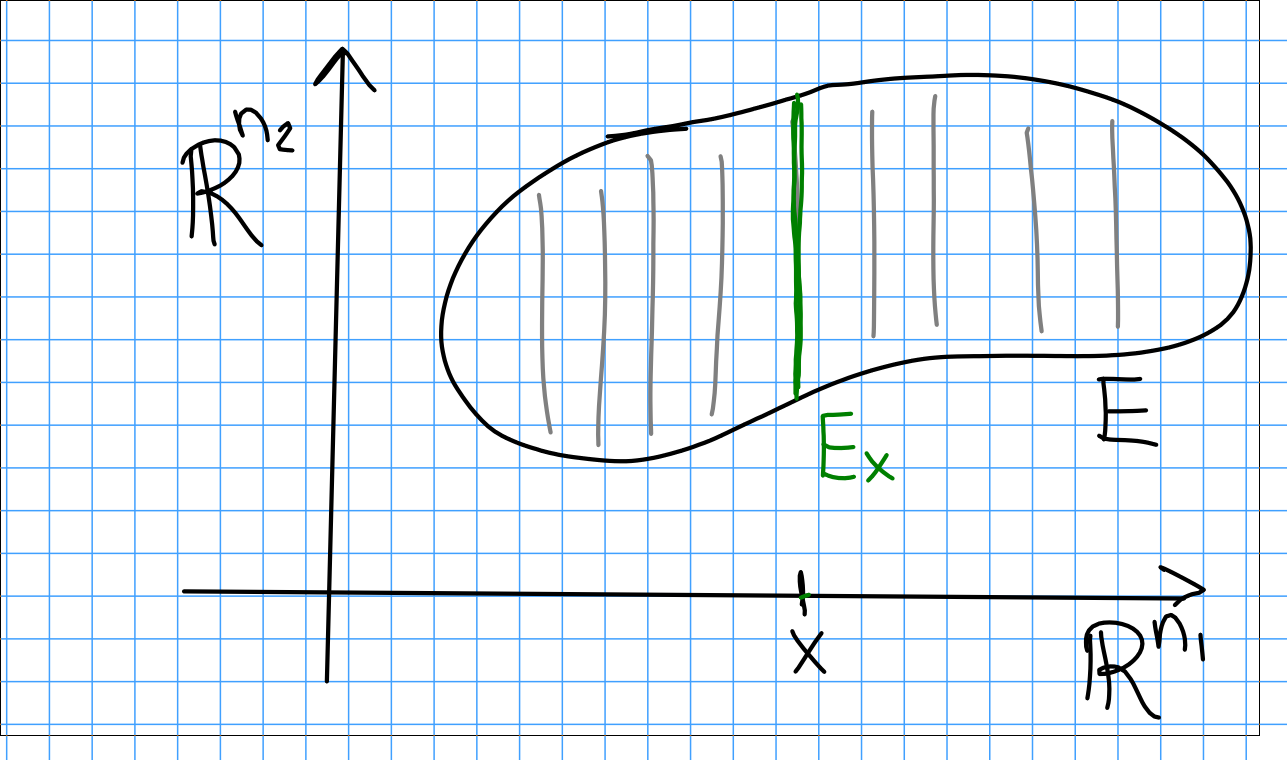
\includegraphics{figures/2019-10-08-11:35.png}\\

\begin{quote}
Note: We need to show that taking a \textbf{cylinder} on a function
(i.e.~given \(f(x)\) and defining \(F(x, y) = f(x)\)) does not destroy
measurability. This is necessary in the context of convolution, since
\(f(x - y)\) will need to be measurable in both variables in order to
apply Tonelli.
\end{quote}

\hypertarget{application-area-under-the-graph}{%
\subsection{Application: Area Under the
Graph}\label{application-area-under-the-graph}}

Suppose \(f \geq 0\) on \(\RR^n\), with no assumption of measurability.

Consider defining the ``area under the graph'' as
\begin{align*}
\mathcal{A} \definedas \theset{(x, y) \in\RR^n \cross \RR \suchthat 0 \leq y \leq f(x)}
.\end{align*}

Then

\begin{enumerate}
\def\labelenumi{\arabic{enumi}.}
\item
  \(f\) is measurable on \(\RR^n\) iff \(\mathcal{A}\) is a measurable
  subset of \(\RR^{n+1}\).
\item
  If \(f\) is measurable on \(\RR^n\), then
  \begin{align*}
  m(\mathcal{A}) = \int_{\RR^n} f = \int_0^\infty m(\theset{x\in\RR^n \suchthat f(x) \geq y}) ~dy
  \end{align*}
\end{enumerate}

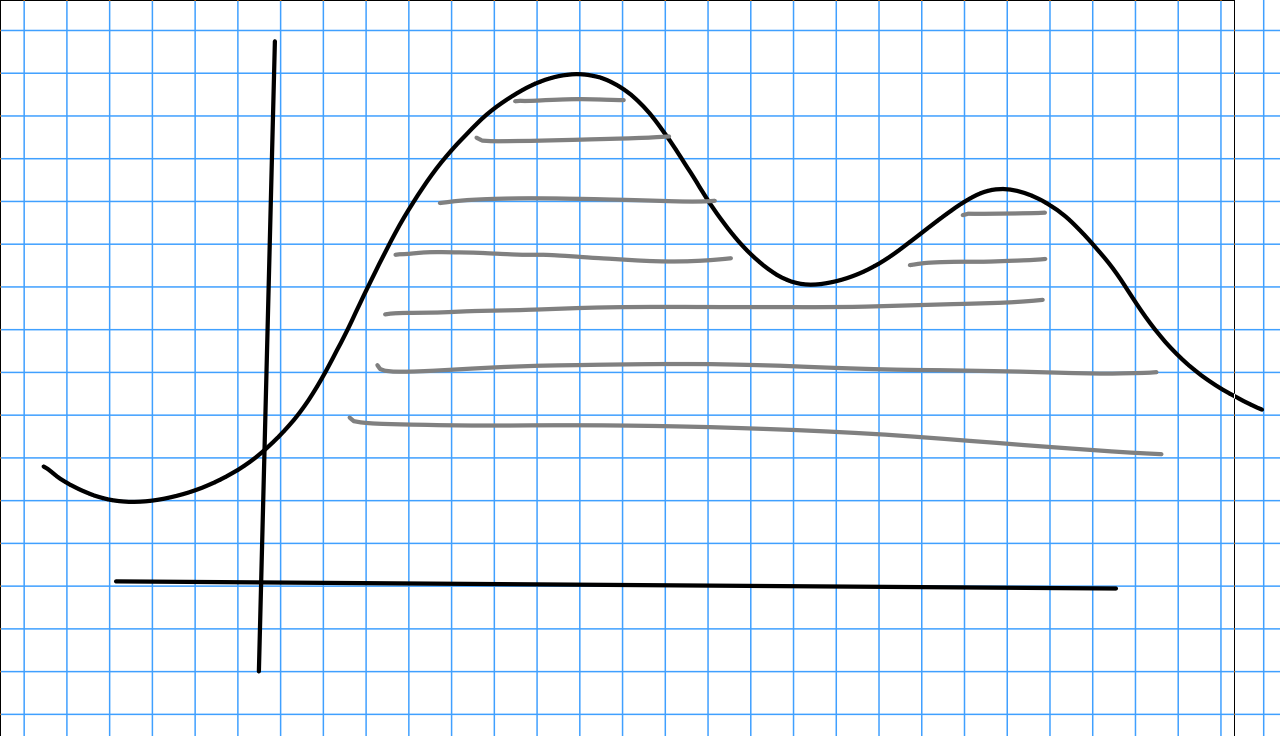
\includegraphics{figures/2019-10-08-11:33.png}\\

\emph{Proof of (1):}

\(\implies:\) Suppose \(f\) is measurable on \(\RR^n\).

By the lemma, \(F(x, y) = f(x)\) is measurable on \(\RR^n \cross \RR\)
and \(G(x, y) = y\) is as well. But then
\(\mathcal{A} = \theset{G \leq F} \intersect \theset{G \geq 0}\), which
is an intersection of measurable sets and thus measurable.

\(\impliedby:\) Suppose \(\mathcal{A}\) is measurable.

By Tonelli, for almost every \(x\in \RR^n\), the slice
\begin{align*}
\mathcal{A}_x = \theset{y \in \RR \suchthat (x, y) \in \mathcal{A}} = [0, f(x)]
\end{align*} is measurable.

Then \(m(\mathcal{A}_x) = f(x)\), so \(x\mapsto \mathcal{A}_x\) is a
measurable function of \(x\) and \(m(\mathcal{A}) = \int f(x) ~dx\).

Repeating this argument with \(y\) slices instead, for almost every
\(y\in \RR\) we have
\begin{align*}
\mathcal{A}_y = \theset{x \in \RR^n \suchthat (x, y) \in \mathcal{A}} = \theset{x\in\RR^n \suchthat f(x) \geq y \geq 0}
,\end{align*} which is a measurable subset of \(\RR^n\).

So it makes sense to integrate it, and
\begin{align*}
m(\mathcal{A}) 
= \int m(\mathcal{A}_y)~dy 
= \int_0^y m(\theset{x \in \RR^n \suchthat f(x) \geq y}) ~dy
.\end{align*}

\(\qed\)

\emph{Alternative proof}:

\begin{align*}
\int_0^\infty m ( \theset{x\in \RR^n \suchthat f(x) \geq y}) 
&= \int_{\RR} \int_{\RR^n} \chi_{S \definedas \theset{x\in \RR^n \suchthat f(x) \geq y \geq 0}} \\
&= \int_{\RR^n} \int_\RR \chi_S \\
&= \int_{\RR^n} \int_0^{f(x)} ~dy~dx \\
&= \int_{\RR^n} f(x)~dx
.\end{align*}

\(\qed\)

\hypertarget{appendix-on-measurability-in-rrn_1-cross-rrn_2.}{%
\subsection{\texorpdfstring{Appendix on Measurability in
\(\RR^{n_1} \cross \RR^{n_2}\).}{Appendix on Measurability in \textbackslash RR\^{}\{n\_1\} \textbackslash cross \textbackslash RR\^{}\{n\_2\}.}}\label{appendix-on-measurability-in-rrn_1-cross-rrn_2.}}

\textbf{Lemma:} If \(f\) is measurable on \(\RR^{n_1}\), then
\(F(x, y) \definedas f(x)\) is measurable on the product space
\(\RR^{n_1} \cross \RR^{n_2}\)

\begin{quote}
Qual problem alert.
\end{quote}

\emph{Proof of Lemma:} Suppose \(f\) is measurable on \(\RR^n\); we want
to show that \(F(x, y) = f(x)\) is measurable on \(\RR^n \cross \RR\).

This amounts to showing that for any \(a\),
\begin{align*}
S_a \definedas \theset{(x,y) \suchthat F(x, y) \geq a} \in \mathcal{M}(\RR^{n+1}).\end{align*}

But we can rewrite
\begin{align*}
S_a = \theset{x\in\RR^n \suchthat f(x) > a} \cross \RR
,\end{align*}

which is the cylinder on a measurable set. As we will show, this is
always measurable.

\begin{quote}
Best way to show measurability: use Borel characterization, or show that
it's an \(H \disjoint N\) where \(H \in F_\sigma\) and \(N\) is null.
\end{quote}

So write \(E = H \disjoint N\) where \(H\in F_\sigma\) and \(N\) is
null.

Then \(E \cross \RR = (H \cross \RR) \union (N \cross \RR)\).

But \(H\cross \RR\) is still an \(F_\sigma\) set, so we just need to
show \(N\cross \RR\) is still null.

We have \(N \cross [-k, k] \nearrow N \cross \RR\), so we can use
continuity from below.

To see that \(m(N \cross [-k, k]) = 0\), first cover \(N\) by such that
\(\sum \abs{Q_i} < \varepsilon / 2k\).

But the measure of any rectangle over such a cube will be
\(M(\overline{Q}_i) = 2 k \cdot m(Q_i)\), which we can pull out of
\(\sum \abs{\overline{Q}_i}\). \(\qed\)

\hypertarget{fubini-and-fubini-tonelli}{%
\subsection{Fubini and Fubini-Tonelli}\label{fubini-and-fubini-tonelli}}

\textbf{Summary}":

\begin{itemize}
\item
  \textbf{Tonelli}: \emph{Non-negative and measurable} allows switching
  integrals,
\item
  \textbf{Fubini}: \emph{Just measurable} allows switching the
  integrals, the integrals are finite, and all iterated variants are
  equal.
\item
  \textbf{Fubini/Tonelli}: Extends switching beyond just non-negative
  integrands.
\end{itemize}

\textbf{Theorem (Fubini):} Let \(f(x, y)\) be an integrable function on
\(\RR^n \cross \RR^{n_1} \cross \RR^{n_2}\).

Then for almost every \(x\in \RR^{n_1}\),

\begin{enumerate}
\def\labelenumi{\arabic{enumi}.}
\item
  \(f_x(y) = f(x, y)\) is an \emph{integrable} function of \(y\) in
  \(\RR^{n_2}\).
\item
  \(\int_{\RR^{n_2}} f(x, y) ~dy\) is an integrable function of \(x\) in
  \(\RR^{n_1}\).
\end{enumerate}

Moreover,
\begin{align*}
\int_{\RR^n} f = \int \int f(x, y) ~dx~dy
\end{align*} in either order.

\textbf{Theorem (Fubini-Tonelli):} Let \(f(x, y)\) be measurable in the
product space.

If either
\begin{align*}
\int \left( \int \abs{f(x, y) ~ dy}\right) ~dx < \infty
\end{align*} or
\begin{align*}
\int \left( \int \abs{f(x, y) ~ dx}\right) ~dy < \infty
\end{align*} then by Tonelli on \(\abs{f(x, y)}\), we can conclude
\(f\in L^1(\RR^{n_1} \cross \RR^{n_2})\).

Moreover, by Fubini, \(\int f\) is equal to either iterated integral.

\begin{quote}
Moral: If \emph{any} iterated integral is finite, then they \emph{all}
are.
\end{quote}

Comparing this to sums: recall that \(\sum \int f_n = \int \sum f_n\) is
true exactly when

\begin{enumerate}
\def\labelenumi{\arabic{enumi}.}
\tightlist
\item
  \(f_n \geq 0\), and
\item
  \(\sum \int \abs{f_n} < \infty\).
\end{enumerate}

\hypertarget{tuesday-october-15}{%
\section{Tuesday October 15}\label{tuesday-october-15}}

\hypertarget{proof-of-fubinis-theorem}{%
\subsection{Proof of Fubini's Theorem}\label{proof-of-fubinis-theorem}}

Recall the strong version of DCT: It allows you to deduce \(L^1\)
converges from a.e. convergence.

Note that otherwise, this are incomparable!

\emph{Proof of Fubini's Theorem}: see book for the gory details.

\begin{quote}
Essentially uses MCT a number of times and reduces to the case of cubes
that possibly include boundaries.
\end{quote}

\hypertarget{thursday-october-17}{%
\section{Thursday October 17}\label{thursday-october-17}}

\hypertarget{review-of-tonelli}{%
\subsection{Review of Tonelli}\label{review-of-tonelli}}

\textbf{Theorem (Tonelli)}: Suppose \(f(x, y)\) is non-negative on
\(\RR^{n_1} \cross \RR^{n_2}\) and measurable on the product space. Then
for a.e. \(x\), we have

\begin{enumerate}
\def\labelenumi{\arabic{enumi}.}
\item
  \(f_x(y)\) is a measurable function of \(y\).
\item
  Since it's non-negative and measurable, the integral makes sense, and
  \begin{align*}
  \int_{\RR^{n_2}} f(x, y) ~dy
  \end{align*} is a measurable function of \(x\).
\item

  \begin{align*}
  \int\int f(x,y) ~dx ~dy = \int\int f(x,y) ~dy~dx = \int f
  .\end{align*}
\end{enumerate}

\emph{Proof:}

\begin{quote}
Qual problem alert: useful technique!
\end{quote}

Essentially use Fubini, and truncate domain/range with a \(k\dash\)ball.

See proof of the \emph{case-jumping lemma} and notes on webpage for
details.

\begin{quote}
We'll never need to dig into the proof of this, but there will
\emph{always} be a question related to \emph{applying} it.
\end{quote}

\hypertarget{measurability-of-linear-transformations}{%
\subsection{Measurability of Linear
Transformations}\label{measurability-of-linear-transformations}}

\textbf{Theorem:} Let \(T \in \GL(n, \RR)\). Then

\begin{itemize}
\item
  \(f\) measurable \(\implies\) \(f\circ T\) is measurable.

  \begin{itemize}
  \tightlist
  \item
    Contrast to what happens for \(g\) a continuous function instead of
    \(T\).
  \end{itemize}
\item

  \begin{align*}
  f \leq 0 \text{ or } f\in L^1 \implies \int f = \abs{\det(T)} \int (f\circ T)(x)
  .\end{align*}
\item

  \begin{align*}
  E \in \mathcal{M}(\RR^n) \implies T(E) \in \mathcal{M}(\RR^n)
  .\end{align*}
\end{itemize}

It suffices to prove this for Borel sets and Borel measurable functions.
This can be proved using Fubini.

Note that if we choose \(f\) to be Borel measurable, then \(f\circ T\)
will be measurable because \(T\) is continuous.

\begin{quote}
This follows because \(\theset{E \suchthat T\inv(E) \in\mathcal{B}}\) is
in fact a \(\sigma\dash\)algebra that contains all open sets.
\emph{Exercise}: Prove this.
\end{quote}

We can also reduce this to proving the result for \(T_i\) an elementary
matrix, since if it holds for \(T,S\) then it holds for \(TS\) because
\begin{align*}
\int f = \det T \int f\circ T = \det T \det S \int f\circ T \circ S = \det(TS) \int f\circ(TS)
\end{align*} But this follows from Fubini-Tonelli.

\begin{quote}
Note that if (3) holds for Borel sets, then (3) holds for Lebesgue null
sets.
\end{quote}

Suppose now that \(f\) is just Lebesgue measurable, and let \(G\) be
open in \(\RR\).

Then \(f\inv(G) = H \union N\) where \(H\in G_\delta\) and \(m(N) = 0\)
and
\begin{align*}
T\inv(f\inv(G)) = T\inv(H) \union T\inv(N)
.\end{align*}

But by the first part, \(T\inv(H)\) is still Borel, and \(T\inv(N)\) is
still null. So \(f\circ T\) is measurable.

\begin{quote}
Note that this kind of thing usually works -- just establish something
Borel sets, then use this characterization to extend it to Lebesgue.
\end{quote}

\hypertarget{tuesday-october-22}{%
\section{Tuesday October 22}\label{tuesday-october-22}}

\hypertarget{convolution}{%
\subsection{Convolution}\label{convolution}}

Recall:

\begin{itemize}
\item
  \textbf{Continuous Compact Approximation:} \(C_c \injects L^1\) is
  dense.
\item
  \textbf{Continuity in \(L^1\):}\\
  \begin{align*}
  f\in L^1 \implies \norm{\tau f - f} \to 0, \text{ i.e. } \lim_{y\to 0} \int \abs{f(x+y) - f(x)} ~dx = 0
  .\end{align*}
\item
  If \(f\in L^1\), then for any \(\varepsilon > 0\),

  \begin{itemize}
  \item
    \textbf{Small tails:} There exists a \(\delta\) such that for all
    \(E\) such that
    \begin{align*}
    m(E) \leq \delta \implies \int_E \abs{f} < \varepsilon
    .\end{align*}
  \item
    There exists an \(N\) such that
    \begin{align*}
    \int_{\theset{\norm{x} \geq N}} \abs{f} < \varepsilon
    .\end{align*}

    \begin{itemize}
    \tightlist
    \item
      Note that \(\abs{f(x)} < \varepsilon ~~\forall x\) such that
      \(\norm x \geq N\) exactly when \(f\) is uniformly continuous
    \end{itemize}
  \end{itemize}
\end{itemize}

\textbf{Definition:} The \emph{convolution} of \(f,g\) measurable
functions on \(\RR^n\) is given by
\begin{align*}
f\star g (x) = \int_{\RR^n} f(x-y) g(y) ~dy
\end{align*} for every \(x\) for which this integral makes sense.

\textbf{Remarks:}

\begin{itemize}
\item
  There are sufficient conditions on \(f,g\) which guarantee that
  \(f\star g\) exists.
\item
  If for some \(x\), the function
  \begin{align*}
  y\mapsto f(x-y)g(y)
  \end{align*} is measurable, then the function
  \begin{align*}
  y\mapsto f(y)g(x-y)
  \end{align*} is also integrable.
\end{itemize}

\begin{quote}
Note that this is just a translation followed by a reflection, which is
still integrable since this operation is in \(\GL(n, \RR))\) and
\(f\star g = g \star f\).
\end{quote}

\hypertarget{properties-of-convolutions}{%
\subsection{Properties of
Convolutions}\label{properties-of-convolutions}}

\textbf{Theorem 1:}

\begin{enumerate}
\def\labelenumi{\alph{enumi}.}
\tightlist
\item

  \begin{align*}
  f\in L^1 \text{ and } g \text{ bounded } \implies f\star g \quad \text{ is bounded  *and* uniformly continuous}.
  \end{align*}
\item

  \begin{align*}
  f,g \in L^1 \text{ and } f,g \text{ bounded } \implies \lim_{\abs{x}\to\infty} (f\star g)(x) = 0
  .\end{align*}
\end{enumerate}

\begin{quote}
Note that (b) immediately follows if it were the case that \(f\star g\)
were uniformly continuous and \emph{integrable}, but we don't
necessarily need integrability for this result.
\end{quote}

\begin{quote}
Note: It is possible to pointwise multiply 2 integrable functions and
get something non-integrable -- consider \(f^2\) where
\begin{align*}
f(x) = \frac{1}{\sqrt x} \chi_{[0,1]}
.\end{align*}
\end{quote}

\textbf{Theorem 2:}

\begin{align*} f,g \in L^1 \implies \norm{f\star g}_1 \leq \norm{f}_1 \norm{g}_1,\end{align*}
and equality is attained if \(f, g \geq 0\).

That is,
\begin{align*}
\int \abs{f\star g} \leq \int\abs{f} \int\abs{g}
.\end{align*}

\textbf{Corollary}: If \(g\) is additionally \emph{bounded}, then
\begin{align*}
\lim_{\abs x \to \infty} f\star g(x) = 0
.\end{align*}

\textbf{Theorem 3:} \begin{align*}
f\in L^1, \quad g \text{ differentiable}, \quad \text{ and } g, \dd{g}{x_1}, \cdots, \dd{g}{x_n} &\text{ all bounded } \implies \\
f\star g \in C^1  
\text{ and }\dd{}{x_j} (f\star g) &= f\star (\dd{}{x_j} g)
.\end{align*}

\textbf{Corollary}:
\begin{align*}
f\in L^1  \text{ and } g\in C^\infty_c \implies f\star g \in C^\infty \text{ and } \lim_{\abs x \to \infty} f\star g(x) = 0
.\end{align*}

In other words, defining \(C_0\) as the functions that vanish at
infinity, we have \(f\star g \in C_0^\infty\).

\begin{quote}
Note that we don't necessarily preserve \emph{compact support} after
this convolution. See the following picture, which looks similar for any
fixed \(x\) -- particularly any large \(x\).
\end{quote}

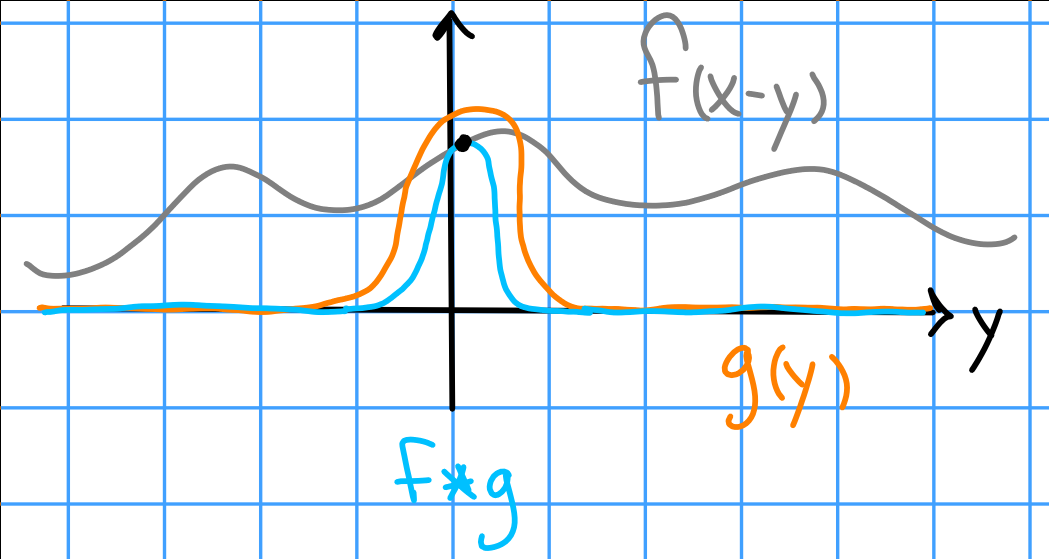
\includegraphics{figures/2019-10-22-11:55.png}\\

\emph{Proof of Theorem 1, part (a):}

\begin{align*}
\abs{\int f(x-y)g(y) ~dy} 
&\leq \int \abs{f(x-y)} \abs{g(y)} ~dy \\
&\leq M \int \abs{f(x-y)} ~dy \\
&\leq M \norm{f}_1
.\end{align*}

and

\begin{align*}
\abs{f\star g(x+h) - f\star g}
&= \abs{
\int f(x+h-y)g(y)~dy - \int f(x-y)g(y)~dy
} \\
&\leq \int \abs{f(x+h-y) - f(x-y)} \abs{g(y)}~dy \\
&\leq M \int \abs{f(z+h) - f(z)}~dz \to 0
.\end{align*}

\emph{Proof of Theorem 1, part (b):}

Let \(\varepsilon > 0\), then choose \(N\) such that
\begin{align*}
\int_{\theset{\norm{y} \geq N}} \abs{f(y)} ~dy < \varepsilon \quad \text{and} \quad 
\int_{\theset{\norm{y} \geq N}} \abs{g(y)} ~dy 
.\end{align*}

Since \(\abs{x} \leq \abs{x-y} + \abs{y}\) by the triangle inequality,
if we take \(\abs{x} \geq 2N\), then \emph{either}

\begin{itemize}
\tightlist
\item
  \(\abs{x-y} \geq N\), or
\item
  \(\abs{y} \geq N\).
\end{itemize}

In the first case, let \(A_x = \theset{\abs x \geq N}\)

\begin{align*}
\abs{f\star g} 
&\leq \int \abs{f(x-y)} \abs{g(y)} ~dy \\
&\leq M \int_{A_{x-y}} \abs{f(x-y)} < M\varepsilon
.\end{align*}

and in the second case, take

\begin{align*}
\abs{f\star g} 
&\leq \int \abs{f(x-y)} \abs{g(y)} ~dy \\
&\leq M \int_{A_{y}} \abs{g(y)} < M\varepsilon
.\end{align*}

\emph{Proof of Theorem 2:}

Since \(f,g \in L^1\), the function \(h(x, y) \definedas f(x-y)g(y)\)
will be measurable on \(\RR^n\cross\RR^n\) as a product of measurable
functions if we can show that the function
\(f_{x,y} \definedas (x,y) \mapsto f(x-y)\) is measurable.

To see that this is the case, define \(F(x-y, y) = f(x-y)\) by taking
the cylinder, then let
\begin{align*}
T = \left( \begin{array}{cc} 1& -1\\  0 & 1 \end{array}\right) \implies T(x, y) = (x-y, y)
,\end{align*}

Thus \(f_{x,y}(x, y) = (F \circ T)(x, y)\).

We can now note that

\begin{align*}
\int \int \abs{f(x-y)} \abs{g(y)} ~dy ~dx 
&=_{FT} \int \int \abs{f(x-y)} \abs{g(y)} ~dx ~dy \\
&= \int \abs{g(y)} \left( \int \abs{f(x-y)} ~dx \right) ~dy \\
&= \norm{f}_1 \norm{g}_1
.\end{align*}

This proves that the integrand is in \(L^1(\RR^{2n})\), so Fubini
implies that \(f\star g(x)\) is in \(L^1\) for almost every \(x\).

But then

\begin{align*}
\int \abs{f\star g(x)}~dx 
&\leq \int \int \abs{f(x-y) g(y)}~dy~dx \\
&= \norm{f}_1 \norm{g}_1
.\end{align*}

\(\qed\)

\begin{quote}
Note that equality is attained here if \(f, g \geq 0\).
\end{quote}

\hypertarget{thursday-october-24}{%
\section{Thursday October 24?}\label{thursday-october-24}}

Todo.

\hypertarget{tuesday-october-29}{%
\section{Tuesday October 29}\label{tuesday-october-29}}

\hypertarget{approximations-of-the-identity}{%
\subsection{Approximations of the
Identity}\label{approximations-of-the-identity}}

\textbf{Theorem:} Let \(\phi \in L^1\) and \(\int \phi = 1\).

Then

\begin{itemize}
\item
  If \(f\) is bounded and uniformly continuous, then
  \(f \ast \phi_t \mapsvia{u} f\) uniformly where
  \begin{align*}
  \phi_t(x) \definedas \frac 1 {t^n} \phi(\frac x t)
  .\end{align*}
\item
  If \(f\in L^1\), then \(f \ast \phi_t \mapsvia{L^1} f\) in \(L_1\).
\end{itemize}

\textbf{Applications:}

\hypertarget{theorem-1-smooth-compactly-supported-functions-are-dense-in-l1}{%
\subsection{\texorpdfstring{Theorem 1: Smooth Compactly Supported
Functions are Dense in
\(L^1\)}{Theorem 1: Smooth Compactly Supported Functions are Dense in L\^{}1}}\label{theorem-1-smooth-compactly-supported-functions-are-dense-in-l1}}

\textbf{Theorem:} \(C_c^\infty \injects L^1\) is dense,

That is, \(\forall \varepsilon > 0\) and for all \(f\in L^1\), there
exists a \(g\in C_c^\infty\) such that \(\norm{f - g}_1 < \varepsilon\).

\emph{Proof:} Since \(C_c^0\) is dense in \(L^1\), it suffices to show
the following:
\begin{align*}
\forall \varepsilon > 0 ~\&~ h \in C_c^1, \quad \exists g\in C_c^\infty \suchthat \norm{h - g}_1 < \varepsilon.
\end{align*}

Let \(\phi \in C_c^\infty\) be arbitrary where \(\int \phi = 1\)
\emph{(which exist!)}.

Then \(\norm{h\ast \phi_t - h}_1 < \varepsilon\) for \(t\) small enough.
It remains to show that \(f\definedas h\ast \phi_t \in C_c^\infty\).

\(f\) is smooth because of theorem 3 regarding convolution, applied
infinitely many times.

\(f\) is also compactly supported: since \(h, \phi_t\) are compactly
supported, so there is some large \(N\) such that
\(\abs x > N \implies h(x) = \phi_t(x) = 0\).

Then if \(\abs x > 2N\), we can note that
\begin{align*}
\abs x \leq \abs{x+y} + \abs{y},
\end{align*} so either \(\abs{x-y}\geq 2N\) or \(\abs y \geq N\).

But then
\begin{align*}
f(x) \definedas h \ast \phi_t(x) = \int h(x-y)\phi_t(y)~dy = 0
,\end{align*} where by the previous statement, at least one term in the
integrand is zero and thus the integral is zero and
\(f \definedas h \ast \phi_t\) compactly supported.

\(\qed\)

\hypertarget{theorem-2-weierstrass-approximation}{%
\subsection{Theorem 2: Weierstrass
Approximation:}\label{theorem-2-weierstrass-approximation}}

\textbf{Theorem:} A function can be \emph{uniformly} approximated by a
polynomial on any closed interval, i.e.
\begin{align*}
\forall\varepsilon > 0,~ f\in C([a, b]),\quad \exists \text{ a polynomial } P \suchthat \abs{f(x) - P(x)} < \varepsilon \quad \forall x\in [a, b].
\end{align*}

\emph{Proof:} Let \(g\) be a continuous function on
\([-M, M] \supseteq [a, b]\) such that
\(\restrictionof{g}{[a, b]} = f\).

Let \(\phi(x) = e^{-\pi x^2}\) be the standard Gaussian, then
\(g \ast \phi_t \uniformlyconverges g\) on \([-M, M ]\), and thus
\(g\ast \phi_t \uniformlyconverges f\) on \([a, b]\).

\begin{quote}
The problem is that this is not a polynomial.
\end{quote}

We can let \(\varepsilon > 0\), then there is a \(t\) such that
\begin{align*}
\abs{g\ast \phi_t(x) - g(x)} < \varepsilon \quad \forall x\in[-M, M]
.\end{align*}

Note that \(\phi_t(x) = \frac 1 t e^{-\pi x^2 / t^2}\), and Maclaurin
expand to obtain
\begin{align*}
P(t) \definedas \frac 1 t \sum_{n=0}^\infty \frac{(-1)^n \pi^n x^{2n}}{t^{2n} n!}
.\end{align*}

\begin{quote}
Note that the Maclaurin series will converge uniformly on compact sets!
\end{quote}

By uniform convergence of \(P\), we can truncate it to bound the
difference by say \(\varepsilon / \norm{g}_1\).

Let \(Q(x)\) be the truncated series. Then

\begin{align*}
\abs{g\ast\phi_t(x) - g\ast Q(x)} \leq \abs{g\ast(\phi_t - Q)(x)} \leq \norm{g} \norm{p_t(x) - Q(x)}_\infty < \varepsilon \to 0,
\end{align*}

where \(\norm{f}_\infty = \displaystyle\sup_{x\in [a, b]} \abs{f(x)}\)
and \((g\ast Q)(x)\) is a polynomial. \(\qed\)

\hypertarget{fourier-transform-on-rrn}{%
\subsection{\texorpdfstring{Fourier Transform on
\(\RR^n\)}{Fourier Transform on \textbackslash RR\^{}n}}\label{fourier-transform-on-rrn}}

Given \(f\in L^1\), we defined the Fourier transform of \(f\) by
\begin{align*}
\hat{f}(\xi) = \int f(x) e^{-2\pi i x\cdot \xi}~dx
.\end{align*}

Some facts we know about the Fourier transform:

\begin{itemize}
\item
  \(f\in L^1 \implies \hat{f}\) is bounded and uniformly continuous.

  (From an old homework!)
\item
  The Riemann-Lebesgue lemma:
  \(\displaystyle\lim_{\abs \xi \to \infty} \hat{f}(\xi) = 0\),
  i.e.~\(\hat{f}\) vanishes at infinity.
\end{itemize}

\begin{quote}
Warning: it is \textbf{not} true that
\(f \in L^1 \implies \hat{f}\in L^1\)!
\end{quote}

\hypertarget{fourier-inversion-formula}{%
\subsubsection{Fourier Inversion
Formula}\label{fourier-inversion-formula}}

\textbf{Theorem (Inversion Formula):} If \(f, \hat{f} \in L^1\) then
\begin{align*}
f(x) = \int \hat{f} (x) e^{2\pi i x\cdot \xi} ~d\xi \quad \text{for a.e. } x,
\end{align*} i.e.~\(\hat{\hat{f}} = f(-x)\), and the Fourier transform
is 4-periodic.

\begin{quote}
Note that there is an interpretation here as writing an arbitrary
function as a (continuous) sum of \emph{characters}, where we're
considering \(\RR^n\) with the action of translation. In this setting,
exponentials are certain eigenfunctions.
\end{quote}

\textbf{Corollaries:}

\begin{enumerate}
\def\labelenumi{\arabic{enumi}.}
\item
  \(f, \hat{f} \in L^1\) implies that \(f\) itself is bounded,
  continuous, and vanishes at infinity. (Note that this is not true for
  arbitrary \(L^1\) functions!)

  \begin{quote}
  We will in fact show that
  \(\theset{f \mid f, \hat{f} \in L^1}\injects L^1\) is dense.
  \end{quote}
\item
  \(f \in L^1\) and \(\hat{f} = 0\) a.e. \(\implies f = 0\) almost
  everywhere

  (Proof uses the Inversion formula)
\end{enumerate}

\emph{Proof of Inversion Formula:}

\begin{quote}
Note: Fubini-Tonelli won't work here \emph{directly}.
\end{quote}

We'll have
\begin{align*}
f(x) = \int\int f(y) e^{-2\pi i y\cdot \xi} e^{2\pi i x \cdot \xi} ~dy ~d\xi,
\end{align*}

which is (obviously?) not in \(L^1(\RR^{2n})\).

So we'll introduce a ``convergence factor''
\(e^{-\pi t^2 \abs{\xi}^2}\), which will make the integral swap result
in something integrable, then take limits.

\textbf{Important example (HW):}
\begin{align*}
g(x) = e^{-\pi \abs{x}^2} \implies \hat{g}(\xi) = e^{-\pi \abs{\xi}^2}
.\end{align*}

Note that
\begin{align*}
g_t(x) = \frac{1}{t^n} e^{-\pi \abs{x}^2 / t^2}
\end{align*} is an approximation to the identity, and \(\int g_t = 1\).

By a HW exercise, have have
\begin{align*}
\hat{g_t}(\xi) = \hat{g}(t\xi) = e^{-\pi t^2 \abs{\xi}^2}
,\end{align*} which is exactly the convergence factor we're looking for.
Moreover, \(f \ast g_t \mapsvia{L^1} f\) in \(L^1\).

\begin{quote}
This says that the Fourier transform ``commutes with dilation'' in a
certain way.
\end{quote}

\textbf{Lemma (Multiplication Formula):} If \(f, g \in L^1\), then an
easy application of Fubini-Tonelli yields
\begin{align*}
\int f \hat{g} = \int \hat{f} g.
\end{align*}

We have

\begin{align*}
\int \hat{f}(\xi) e^{-\pi t^2 \abs{\xi}^2} e^{2\pi i x \cdot \xi} ~d\xi 
&\definedas 
\int \hat{f}(\xi) \phi(\xi) \quad \quad (= f \ast g_t(x) \mapsvia{L_1} f) \\
&= \int f(y) \hat{\phi}(y)~dy \\
&=_{DCT} \int \hat{f}(\xi) e^{2\pi i x \cdot \xi} ~d\xi 
\quad \text{as } t\to 0
.\end{align*}

where \(\phi(\xi) = e^{2\pi i x\cdot \xi} \hat{g_t}(\xi)\).

\begin{quote}
By a HW problem, we know
\begin{align*}
\hat{\phi}(y) = \hat{\hat{g}_t}(y-x) =  g_t(x - y)
.\end{align*}
\end{quote}

But now one term is converging to
\(\int \hat{f}(\xi) e{2\pi i x\cdot \xi} ~d\xi\) as \(t\to 0\)
pointwise, and \(f\ast g_t(x) \to f\) as \(t\to 0\) in \(L_1\).

So there is a subsequence of the latter term converging to \(f\) almost
everywhere, and thus the pointwise limit in the first is equal to the
\(L^1\) limit in the second.

We thus obtain
\begin{align*}
f(x) = \int \hat{f}(\xi) e^{2\pi i x\cdot \xi} ~d\xi
\end{align*} almost everywhere.

\(\qed\)

\hypertarget{thursday-october-31}{%
\section{Thursday October 31}\label{thursday-october-31}}

Today: Some topics in PDEs.

\hypertarget{the-heat-diffusion-equation-in-the-plane}{%
\subsection{The Heat / Diffusion Equation in the
Plane}\label{the-heat-diffusion-equation-in-the-plane}}

Setup: Let \(\vector \in \RR^2\) be a plate, and consider it evolving
over time \(t\).

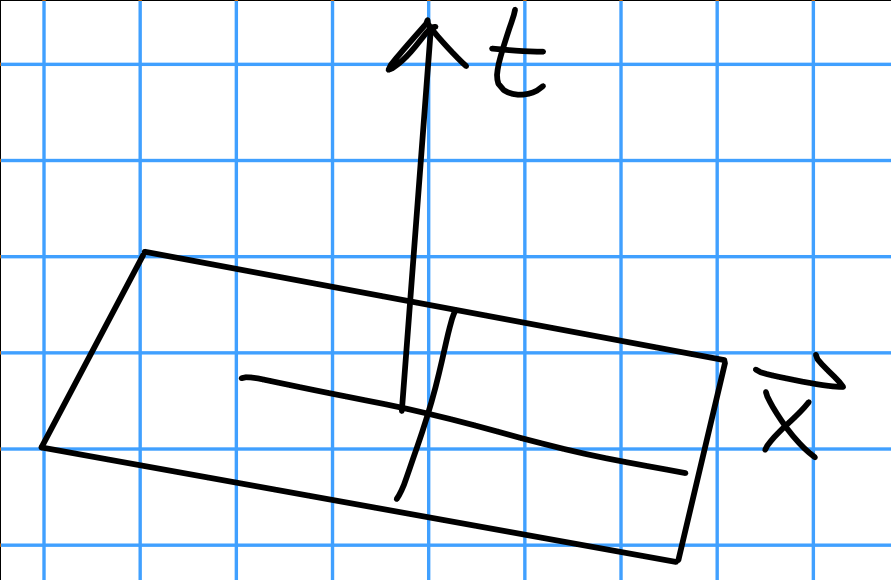
\includegraphics{figures/2019-10-31-11:29.png}\\

So we have pairs \((x, t) \in \RR^2 \cross \RR_{\geq 0}\).

We have some initial distribution of heat on the plate, we want to know
how it evolves over time.

This is modeled by the equation

\begin{align*}
\dd{u}{t} = \frac{1}{4\pi} \left( \dd{^2 u}{x_1^2} + \dd{^2u}{x_2^2} \right) \definedas \frac{1}{4\pi} \Delta u\\
u(x, 0) = f(x)
.\end{align*}

Consider a point and a small ball around that point. Then heat flow at
any point \(x_0\) is given by \(\nabla_x u(x_0, t)\). Now think about
the change in energy contained in this ball. We should have

\begin{align*}
\dd{}{t} \int_{B} u(x, t) ~dx &= \text{Flux across boundary} \\
&= \int_B \nabla \cdot \nabla_x u(x, t) ~dx \quad  \text{by Green's/Divergence theorem} \\
&\definedas \int_B \Delta_x u(x, t) ~dx,
.\end{align*}

which is the heat equation.

\hypertarget{solution}{%
\subsubsection{Solution}\label{solution}}

We can use Fourier transforms to help solve these. Recall the
identities:

\begin{itemize}
\tightlist
\item
  \(\widehat{\dd{}{x_j} f}(\xi) = 2\pi i \xi_j \widehat{f}(\xi)\).
\item
  \(\widehat{\dd{^2}{x_j^2} f}(\xi) = (2\pi i \xi_j)^2\widehat{f}(\xi) = - 4\pi^2 \xi^2 \hat{f}(\xi)\).
\item
  \(\widehat{\Delta f}(\xi) = 4\pi^2 \abs{\xi}^2 \hat{f}(\xi)\).
\end{itemize}

If we take the Fourier transform in the \(x\) variable, we get
\begin{align*}
\widehat{\dd{u}{t}} 
= \dd{}{t} \hat{u}(\xi, t) 
= -\pi \abs{\xi}^2 \hat{u}(\xi, t)
.\end{align*}

Then the boundary conditions become \(\hat{u}(\xi, 0) = \xi{f}(\xi)\).
But note that this is now a first order ODE!

This is easy to solve, we get
\begin{align*}
\hat{u} (\xi, t) = c(\xi) e^{-\pi \abs{\xi}^2 t} = \hat{f}(\xi) e^{-\pi \abs{\xi}^2 t}
.\end{align*}

But then
\begin{align*}
e^{-\pi \abs{\xi}^2 t} = \hat{G} (\sqrt t \xi)
\end{align*} where \(G(x) = e^{-\pi \abs{x}^2}\).

We now have \(\hat{u} = \hat{f} \hat{G} = \widehat{f\ast G}\), but
\textbf{if the transforms are equal then the original functions are
equal by the inversion formula}.

We thus obtain
\begin{align*}
u(x, t) = f \ast G_{\sqrt t}(x) \text{ where } G_{\sqrt t}(x) = \frac{1}{t^{n/2}} e^{-\pi \abs{x}^2/ t}
.\end{align*}

Note that \(f \ast g \to f\) as \(t \to 0\), which matches with the
original boundary conditions, and \(f \ast g \to 0\) as
\(t \to \infty\), which corresponds with heat dissipating.

\hypertarget{dirichlet-problem-in-the-upper-half-plane}{%
\subsection{Dirichlet problem in the upper
half-plane}\label{dirichlet-problem-in-the-upper-half-plane}}

Setup:

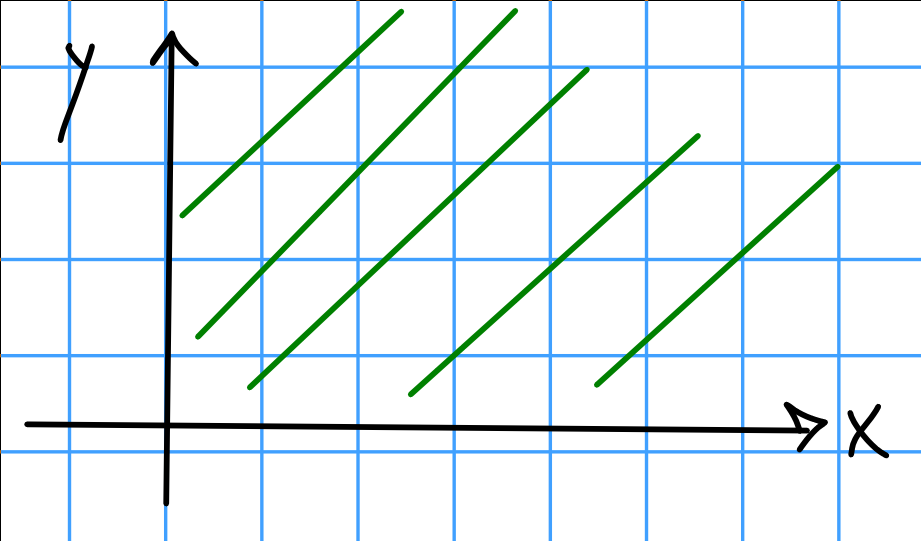
\includegraphics{figures/2019-10-31-11:28.png}\\

We want to solve

\begin{align*}
\Delta u  &= 0 \\
u(x, 0)   &= f(x)
.\end{align*}

\hypertarget{solution-1}{%
\subsubsection{Solution}\label{solution-1}}

We'll use the same technique as the heat equation, and obtain
\begin{align*}
\Delta u = 0 \implies -4\pi^2 \abs{\xi}^2 \hat{u} (\xi ,y) + \dd{^2}{y^2} \hat{u} (\xi, y) = 0
\end{align*}

But this is a homogeneous second order ODE, so we can look at the
auxiliary polynomial. If we have distinct roots, the general solution is
\(c_1 e^{r_1x} + c_2 e^{r_2 x}\).

We thus obtain
\begin{align*}
\hat{u}(\xi, y) = A(\xi) e^{-2\pi \abs{\xi} y} + B(\xi) e^{2\pi \abs{\xi} y}
\end{align*}

In particular, we can just take the first term, since the second term
won't vanish at infinity. We again find that \(A(\xi) = \hat{f}(\xi)\)
by checking initial conditions, so
\begin{align*}
\hat{u}(\xi, y) = \hat{f}(\xi) \hat{P}(y\xi) = \widehat{f \ast P_y}
\quad \text{ where } P(x) = \frac{1}{\pi} \frac{1}{1+x^2}
,\end{align*} and \(f\ast P_y \to f\) as \(y\to 0\) as desired. . \#\#
Wave Equation (Cauchy Problem in \(\RR^n\))

Same situation as the heat equation, but now in
\(\RR^n \cross \RR_{\geq 0}\):

\begin{align*}
\dd{^2 u}{t^2} = \Delta_x u \\
u(x, 0) = f(x) \\
\dd{u}{t}(x, 0) = g(x)
.\end{align*}

This models something like plucking a string with initial shape \(f\)
and initial velocity \(g\).

\begin{quote}
Note that this now involves a \emph{second} derivative!
\end{quote}

\hypertarget{solution-2}{%
\subsubsection{Solution}\label{solution-2}}

Using the same technique, we have

\begin{align*}
\dd{^2}{t^2} \hat{u}(\xi, t) &= -4\pi^2 \abs{\xi}^2 \hat{u} (\xi, t) \\
\hat{u}(\xi, 0) &= \hat{f}(\xi) \\
\dd{}{t} \hat{u}(\xi, 0) &= \hat{g}(\xi)
.\end{align*}

This is again 2nd order linear homogeneous, except there is now a
complex conjugate pair of roots, so we get
\begin{align*}
\hat{u}(\xi, t) = \hat{f}(\xi) \cos(2\pi \abs \xi t) + \frac{\hat{g}(\xi) \sin(2\pi \abs \xi t)}{2\pi \abs \xi}.
\end{align*}

Note that the derivative of the first term is exactly the second term,
so we have

\begin{align*}
u(x, t) = f\ast \dd{}{t} W_t(x) + g\ast W_t(x), \quad \hat{W_t}(\xi) = \frac{\sin(2\pi \abs \xi t)}{2\pi \abs \xi}.
\end{align*}

From the homework problems, we know:

\begin{itemize}
\item
  \(n=1\) implies \(\chi_{[-1, 1]} (x)\)
\item
  \(n = 2\) implies \(\frac{1}{\sqrt{1 - \abs{x}^2}} \chi_{-1, 1}(x)\)
\item
  \(n=3\) implies we only get a measure, i.e.~\(w(x) = \sigma(x)\) where
  \(\sigma\) is a surface measure on \(S^2\).
\item
  For \(n > 3\), \(W\) is a \emph{distribution}.
\end{itemize}

Note that there is a solution given by D'Alembert,
\begin{align*}
u(x, t) = \frac{1}{2} ( f(x +t) + f(x - t) ) + \frac{1}{2} \int_{x-t}^{x+t} g(y) ~dy
\end{align*}

Note the similarities -- the first term is a rough average, the second
term is a more continuous average.

\emph{Exercise}: Verify that these two solutions are equivalent.

\hypertarget{tuesday-november-5}{%
\section{Tuesday: November 5}\label{tuesday-november-5}}

\hypertarget{hilbert-spaces}{%
\subsection{Hilbert Spaces}\label{hilbert-spaces}}

\begin{quote}
See notes on the webpage.
\end{quote}

\textbf{Definition}: An \emph{inner product} on a vector space satisfies

\begin{itemize}
\item
  \(\inner{ax + by}{z} = a \inner{x}{z} + b\inner{y}{z}\) i.e., for all
  fixed \(z\in V\), the map \(x \mapsto \inner{x}{z}\) is a \emph{linear
  functional}.
\item
  \(\inner{x}{y} = \overline{\inner{y}{x}}\)
\item
  \(\inner{x}{x} \in (0, \infty)\)
\end{itemize}

This induces a \emph{norm}, \(\norm{x} = \inner{x}{x}^{1/2}\).

\textbf{Proposition 1:} The map \(x \mapsto \norm{x}\) does in fact
define a norm.

\begin{quote}
The key to establishing this is the triangle inequality, since many of
the other necessary properties fall out easily.
\end{quote}

We'll need the \textbf{Cauchy-Schwarz inequality}, i.e.
\begin{align*}
\abs{\inner{x}{y}} \leq \norm{x} \norm{y},
\end{align*}

with equality iff \(x = \lambda y\).

\begin{quote}
Note that this relates an inner product to a norm, as opposed to other
inequalities which relates norms to other norms.
\end{quote}

\textbf{A useful computation}:

\begin{align*}
\norm{x + y}^2 
&= \inner{x+y}{x+y} \\
&= \norm{x}^2 + 2\mathrm{Re}\inner{x}{y} + \norm{y}^2 \\
&\leq \norm{x}^2 + \abs{\inner{x}{y}} + \norm{y}^2 \\
&\leq \norm{x}^2 + 2\norm{x}\norm{y} + \norm{y}^2 \quad\quad\text{by Schwarz} \\
&= (\norm{x} + \norm{y})^2
.\end{align*}

\textbf{Definition:} An inner product space that is \emph{complete} with
respect to \(\norm{\wait}\) induced from its inner product is a
\emph{Hilbert space}.

\begin{quote}
Recall that a Banach space is a complete \emph{normed} space.
\end{quote}

\emph{Examples:}

\begin{itemize}
\item

  \begin{align*}
   \CC^n \text{ with } \inner{x}{y} = \sum x_j \overline{y_j}
   .\end{align*}
\item

  \begin{align*}
    \ell^2(\NN) \text{ with } \inner{x}{y} = \sum_{j=1}^\infty x_j y_j
    .\end{align*}

  Note that this is finite by \textbf{AMGM}, since by assumption
  \begin{align*}
    \sum x_i y_i \leq \frac 1 2 (\sum x_i + \sum y_i) < \infty
    .\end{align*}
\item

  \begin{align*}
    L^2(\RR^n) \text{ with } \inner{f}{g} = \int f \overline{g}
    .\end{align*}

  This is also finite because
  \begin{align*}
    \int \abs{f\overline g} \leq \frac 1 2 (\int f + \int g)
    .\end{align*}
\end{itemize}

\textbf{Proof of Schwarz Inequality:}

If \(x= \lambda y\) for some \(\lambda \in \CC\), we have equality since
\begin{align*}
\inner{x}{y} = \inner{\lambda y}{y} = \abs{\lambda} \norm{y}^2 = \norm{x}\norm{y}
.\end{align*}

So we can assume \(x-\lambda y \neq 0\) for \emph{any}
\(\lambda \in \CC\), so
\begin{align*}
\inner{x-\lambda y} {x-\lambda y} > 0
.\end{align*}

We thus have
\begin{align*}
0 < \inner{x-\lambda y} {x-\lambda y} =
\norm{x}^2 - 2\overline{\lambda} \mathrm{Re}\inner{x}{y} + \abs{\lambda}^2 \norm{y}
.\end{align*}

Now let \(\lambda = tu\) where \(t\in \RR\) and
\(u =\inner{x}{y} / \abs{\inner{x}{y}}\).

Then we get \(0 < \norm{x}^2 - 2t\abs{\inner{x}{y}} + t^2 \norm{y}^2\)

But this is quadratic in \(t\) and doesn't have a real root, so its
discriminant must be negative.

Thus
\begin{align*}
4\abs{\inner{x}{y}}^2 - 4\norm{y}^2 \norm{x}^2 < 0
,\end{align*} which yields Cauchy-Schwarz.

\(\qed\)

\hypertarget{continuity-of-norm-and-inner-product}{%
\subsection{Continuity of Norm and Inner
Product}\label{continuity-of-norm-and-inner-product}}

\textbf{Application of the Schwarz Inequality:}

If \(x_n \to x\) in \(V\), i.e.~\(\norm{x_n - x} \to 0\), and similarly
\(y_n \to y\), we have \(\inner{x_n}{y_n} \to \inner{x}{y}\) in \(\CC\).

\emph{Proof:}

We have

\begin{align*}
\abs{ \inner{x_n}{y_n} - \inner{x}{y} } &= \abs{ \inner{x_n - x}{y} + \inner{x}{y_n - y} } \\
&\leq \abs{\inner{x_n - x}{y}} + \abs{\inner{x}{y_n - y}} \\
&\leq \norm{x_n - x}\norm{y} + \norm{x} \norm{y_n - y}\quad\quad\text{by Schwarz} \\
& \to 0
.\end{align*}

\(\qed\)

\emph{Exercise}: Show \(\norm{y_n - y} \to 0\) iff
\(\norm{y_n} \to \norm{y}\).

\textbf{Proposition (Parallelogram Law):}

Let \(H\) be an inner product space, then
\begin{align*}
\norm{x+y}^2 + \norm{x-y}^2 = 2(\norm{x}^2 + \norm{y}^2)
\end{align*}

\emph{Exercise}: Prove using parallelogram diagram.

\emph{Proof:} Use the fact that
\begin{align*}
\norm{x \pm y}^2 + \norm{x}^2 \pm 2\mathrm{Re}\inner{x}{y} + \norm{y}^2
,\end{align*} so just add and the cross-terms will cancel.

\textbf{Proposition (Pythagorean Theorem):}
\begin{align*}
\inner{x}{y} = 0 \implies \norm{x+y}^2 = \norm{x}^2 + \norm{y}^2.
\end{align*}

In this situation, we say \(x,y\) are \emph{orthogonal}.

\textbf{Corollary:} If \(\theset{x_i}\) are all pairwise orthogonal,
then
\begin{align*}
\norm{\sum x_i}^2 = \sum \norm{x_i}^2
.\end{align*}

\hypertarget{orthonormal-sets}{%
\subsection{Orthonormal Sets:}\label{orthonormal-sets}}

\textbf{Definition:} A countable collection \(\theset{u_n}\) is
\emph{orthonormal} iff

\begin{enumerate}
\def\labelenumi{\arabic{enumi}.}
\tightlist
\item
  \(\inner{u_j}{u_k} = 0\) for \(j\neq k\), and
\item
  \(\inner{u_j}{u_j} = \norm{u_j}^2 = 1\) for all \(j\).
\end{enumerate}

\begin{quote}
Note: we only consider countable collections; a \emph{separable} Hilbert
space always has such a basis.
\end{quote}

\textbf{Definition:} We say \(\theset{u_n}\) is an orthonormal
\emph{basis} for \(H\) if \(\mathrm{span} \theset{u_n}\)
(i.e.~\emph{finite} linear combinations of \(u_n\)) is dense in \(H\).

\hypertarget{best-approximation-and-bessels-inequality}{%
\subsection{Best Approximation and Bessel's
Inequality}\label{best-approximation-and-bessels-inequality}}

\textbf{Theorem:} Let \(\theset{u_n}\) be a countable orthonormal basis
of \(H\). Then for any \(x\in H\), the \emph{best approximation} to
\(x\) by a sum \(\sum_{n=1}^N a_n u_n\) when \(a_n = \inner{x}{u_n}\).

\begin{quote}
Note: these \(a_n\) will be Fourier coefficients later!
\end{quote}

\emph{Proof:}

\begin{align*}
\norm{x - \sum a_n u_n}^2 
&= \norm{x}^2 - 2\mathrm{Re} \sum \inner{x}{u_n}a_n + \sum \abs{a_n}^2 \\
&= \norm{x}^2 - \sum \abs{\inner{x}{u_n}}^2 + \sum\left( \abs{\inner{x}{u_n}}^2 - 2\mathrm{Re}\inner{x}{u_n}a_n + \abs{a_n}^2  \right) \\
&\leq \norm{x}^2 - \sum \abs{\inner{x}{u_n}}^2 + \abs{\inner{x}{u_n} - a_n  }^2 
&\geq 0
,\end{align*}

where equality is attained iff \(a_n = \inner{x}{u_n} = a_n\). So this
is the best approximation.

\begin{quote}
Note: Equalities are somehow easier to show -- they necessarily involve
direct computations.
\end{quote}

But then
\begin{align*}
0 \leq \norm{x - \sum \inner{x}{u_n} u_n}^2 = \norm{x}^2 - \sum \abs{\inner{x}{u_n}}^2,
\end{align*}

so \(\sum \abs{\inner{x}{u_n}}^2 \leq \norm{x}^2\) holds for every
\(N\), and thus for the infinite sum, which is \textbf{Bessel's
inequality}.

\begin{quote}
If this is an equality, then this is exactly \textbf{Parseval's
theorem}.
\end{quote}

\hypertarget{riesz-fischer}{%
\subsection{Riesz-Fischer}\label{riesz-fischer}}

\textbf{Theorem (Riesz-Fischer):}

\begin{enumerate}
\def\labelenumi{\arabic{enumi}.}
\item
  The map
  \begin{align*}
  x \mapsvia{ \hat{} } \inner{x}{u_n} \definedas \hat{x}(n)
  \end{align*} maps \(H\) onto \(\ell^2\) surjectively.
\item
  If \(\theset{u_n}^\infty\) is orthonormal in \(H\) and
  \(\theset{a_n}^\infty \in \ell^2(\NN)\), then there exists an
  \(x\in H\) such that \(\inner{x}{u_n} = a_n\) for all \(n\in N\).
\item
  \(x\) can be chosen such that \(\norm{x} = \sqrt{\sum \abs{a_n}^2}\).
\end{enumerate}

\emph{Remarks:}

This is not a bijection: there may not be a unique such \(x\). The
\(a_n\) are referred to as the \emph{Fourier coefficients}.

If
\begin{align*}
a_n = 0 \text{ for all } n \implies x=0
,\end{align*} then the set \(\theset{u_n}\) is said to be
\textbf{complete}.

This turns out to be equivalent to \(\theset{u_n}\) being a
\emph{basis}, which is equivalent to the convergence of Fourier series.

\hypertarget{thursday-november-7}{%
\section{Thursday November 7}\label{thursday-november-7}}

\hypertarget{bessel}{%
\subsection{Bessel}\label{bessel}}

Let \(H\) be a Hilbert space, then we have

\textbf{Theorem (Bessel's inequality)}:

If \(\theset{u_n}\) is orthonormal in \(H\), then for any \(x \in H\) we
have equation 0
\begin{align*}
\sum_n \abs{\inner{x}{u_n}}^2 \leq \norm{x}^2,
\end{align*}

or equivalently \(\theset{ \inner{x}{u_n} } \in \ell^2 \NN\).

\emph{Proof:}

We have

\begin{equation}
0 \leq \norm{
x - \sum_{n=1}^N \inner{x}{u_n} u_n
}^2 =
\norm{x}^2 - \sum_{n=1}^N \abs{
\inner{x}{u_n}
}^2 \forall N
.\end{equation}

\textbf{Remark (Characterization of Basis):}

TFAE:

\begin{itemize}
\item

  \begin{align*}\mathrm{span} \theset{u_n} = H,\end{align*} i.e.~\(u_n\)
  is a basis.
\item

  \begin{align*}\sqrt{ \sum_n \abs{ \inner{x}{u_n}  }^2  } = \norm{x} \forall x\in H,\end{align*}
  i.e.~\textbf{Parseval's identity}
\item

  \begin{align*}\lim_{N\to\infty} \norm{ x - \sum_n^N \inner{x}{u_n}  } = 0,\end{align*}

  i.e.~the Fourier series converges in \(H\).
\end{itemize}

Recall the Riesz-Fischer theorem:

If \(\theset u_n\) is orthonormal in \(H\) and
\(\theset a_n \in \ell^2(\NN)\), then
\begin{align*}
\exists x\in H \text{ such that } a_n = \inner{x}{u_n} \text{ and } \norm{x}^2 = \sum_n \abs{a_n}^2.\end{align*}

Moreover, the map \(x \mapsto \hat{x}(u) \definedas \inner{x}{u_n}\)
maps \(H\) onto \(\ell^2(\NN)\) surjectively.

\emph{Remark}: This \(x\) is only unique if \(\theset u_n\) is
\emph{complete},
i.e.~\(\inner{y}{u_n} = 0 \quad \forall n \implies y = 0\).

\emph{Proof:} Let \(S_N \definedas \sum_{n=1}^N a_n u_n\).

Then \(S_N\) is Cauchy, so

\begin{align*}
\norm{S_N - S_M}^2 &= \norm{ \sum_{n=M+1}^N a_n u_n }^2 \\
&= \sum_{n=M+1}^N  \norm{a_n u_n}^2 \quad\quad\text{by Pythagoras since the $u_n$ are orthogonal} \\
&= \sum_{n=M+1}^n \abs{a_n} \to 0
,\end{align*}

since \(\sum \abs{a_n} < \infty\) implies that the sum is Cauchy.

Since \(H\) is complete, \(S_N \to x\) for some \(x\in H\).

We now need to argue that \(a_n = \inner{x}{u_n}\).

If \(N \geq n\), then we have the identity
\begin{align*}
\abs{\inner{x}{u_n} - a_n} = \abs{\inner{x}{u_n} - \inner{S_N}{u_n}  } = \abs{ \inner{x - S_N}{u_n} } \leq \norm{x - S_N} \to 0.
\end{align*}

\begin{quote}
Note: should be able to translate this to statements about epsilons
almost immediately!
\end{quote}

But then equation 1 holds in the limit as \(N \to \infty\), which
establishes equation 0. \(\qed\)

\emph{Proof of characterization of basis:}

\(1 \implies 2\): Let \(\varepsilon > 0, x\in H, \inner{x}{u_n} = 0\)
for all \(n\). We will attempt to show that \(\norm{x} < \varepsilon\),
so \(x = 0\).

By (1), there is a \(y\in \mathrm{span}\theset{u_n}\) such that
\(\norm{x - y}< \varepsilon\). But then \(\inner{x}{y} = 0\), so
\begin{align*}
\norm{x}^2 = \inner{x}{x} = \inner{x}{x-y} \leq \norm{x}{x-y} \leq \varepsilon \norm {x} \to 0
.\end{align*} \(\qed\)

\begin{quote}
Note: \(\inner{x}{x} = \inner{x}{x} - \inner{x}{y} = \inner{x}{x-y}\)
since \(\inner{x}{y} = 0\).
\end{quote}

\(2 \implies 3\): By Bessel, we have
\(\theset{\inner{x}{u_n} } \in \ell^2 \NN\), and we know that its norm
is bounded by \(\norm{x}\).

By Riesz-Fischer, there exists a \(y\in H\) such that
\(\inner{y}{u_n} = \inner{x}{u_n}\) and
\(\norm{y} = \sqrt{ \sum \abs{\inner{x}{u_n}}^2 }\).

By completeness, we get \(x=y\). \(\qed\)

\hypertarget{existence-of-bases}{%
\subsection{Existence of Bases}\label{existence-of-bases}}

\begin{itemize}
\item
  Every Hilbert space has an orthonormal basis (possibly uncountable)
\item
  \(H\) \emph{separable} Hilbert space \(\iff\) \(H\) has a
  \emph{countable} basis (separable = countable dense subset).
\end{itemize}

Some examples of orthonormal bases:

\begin{itemize}
\item

  \begin{align*}
  \ell^2 \NN: \quad u_n(k) = \vector e_n \definedas \begin{cases} 1 & n=k \\ 0 & \text{otherwise}\end{cases}
  \end{align*}
\item

  \begin{align*}
  L^2([0,1]):\quad e_n(x) \definedas e^{2\pi i n x}
  .\end{align*}

  Normed: by Cauchy-Schwarz, but need to show it's complete. Can use the
  fact that \(L^1\) is complete.

  Note that
  \begin{align*}
  \inner{f}{e_n} = \int_0^1 f(x) e^{-2\pi i n x} ~dx
  ,\end{align*} which is exactly the Fourier coefficient.
\end{itemize}

\hypertarget{l2-is-complete-sketch}{%
\subsection{\texorpdfstring{\(L^2\) is Complete
(Sketch)}{L\^{}2 is Complete (Sketch)}}\label{l2-is-complete-sketch}}

\emph{Sketch proof that \(L^2([0, 1])\) is complete:}

Note that \(L^2([0, 1]) \subseteq L^1([0, 1])\), since
\begin{align*}
f\in L^2 \implies \int_0^1 \abs{f} \cdot 1 ~dx \leq \sqrt{\int_0^1 \abs{f}^2}
\end{align*} by Cauchy-Schwarz. This also shows that
\(\norm{f}_1 \leq \norm{f}_2\).

Let \(f_n\) be Cauchy in \(L_2\). Then \(f_n\) is Cauchy in \(L^1\), and
since \(L^1\) is complete, there is a subsequence converging to \(f\)
almost everywhere.

By Fatou,
\begin{align*}
\int \liminf_k \abs{f_{n_j} - f_{n_k}}^2 \leq \liminf \int \abs{f_{n_j} - f_{n_k}}
.\end{align*}

But the LHS goes to \(\int \abs{f_{n_j} - f}\) and the RHS is
\(\norm{f_{n_j} - f_{n_k}} \to 0\), so less than \(\varepsilon\) if
\(j\) is big enough. So \(f_{n_j} \mapsvia{L^2} f\) in \(L^2\) as
\(j\to\infty\), and thus \(f_n \to f\in L^2\) as \(n\to\infty\).

\hypertarget{unitary-maps}{%
\subsection{Unitary Maps}\label{unitary-maps}}

\textbf{Definition:} Let \(U: H_1 \to H_2\) such that
\(\inner{Ux}{Uy} = \inner{x}{y}\), i.e.~\(U\) preserves angles, and we
say \(U\) is \emph{unitary}.

Then \(\norm{Ux} = \norm{x}\), i.e.~\(U\) is an \emph{isometry}.

Every unitary map is an isometry. If \(U\) is surjective, this
implication can be reversed.

For example, taking the Fourier transform yields
\begin{align*}
\sum \abs{\hat{f}(u)}^2 = \norm{f}_2^2 = \int\abs{f}^2 \text{ and } \sum \hat{f}(u) \overline{\hat{g}(u)} = \int f \overline{g}
.\end{align*}

\textbf{A corollary of Riesz-Fischer:} If \(\theset u-N\) is an
orthonormal basis in \(H\), then the map
\(x \mapsto \hat{x}(u) \definedas \inner{x}{u_n}\) is a \emph{unitary}
map from \(H\) to \(\ell^2\).

So all Hilbert spaces are unitarily equivalent to \(\ell^2 \NN\).

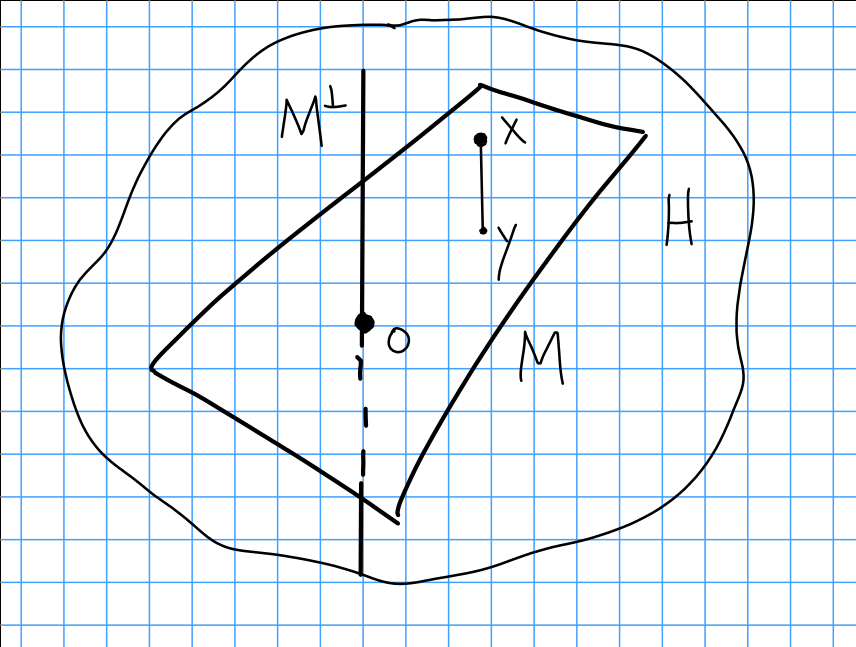
\includegraphics{figures/2019-11-07-12:22.png}\\

\begin{quote}
Subspaces in Hilbert spaces don't have to be closed, but orthogonal
complements are always closed! See homework problem.
\end{quote}

\hypertarget{tuesday-november-12}{%
\section{Tuesday November 12}\label{tuesday-november-12}}

\hypertarget{closed-subspaces-and-orthogonal-projections}{%
\subsection{Closed Subspaces and Orthogonal
Projections}\label{closed-subspaces-and-orthogonal-projections}}

\textbf{Definition:} Let \(H\) be a Hilbert space, then a subspace
\(M \subseteq H\) is \emph{closed} if \(x_n \mapsvia{H} x\) with
\(\theset{x_n} \subset M\) implies that \(x\in M\).

\begin{quote}
Note that finite-dimensional subspaces are \emph{always} closed, so this
is a purely infinite-dimensional phenomenon.
\end{quote}

\textbf{Proposition:} Given any \emph{set} \(M\), then
\begin{align*}
M^\perp \definedas \theset{x\in H \suchthat \inner{x}{y} = 0 ~\forall y\in M}
\end{align*} is always a closed subspace.

\emph{Proof:} Homework problem.

\textbf{Lemma:} Let \(M\) be a closed subspace of \(H\) and \(x\in H\).
Then

\begin{enumerate}
\def\labelenumi{\arabic{enumi}.}
\item
  There exists a unique \(y \in M\) that is \emph{closest} to \(y\),
  i.e.~
  \begin{align*}
  \exists y\in M \suchthat \norm{x - y} = \inf_{y' \in M}\norm{x - y'}
  .\end{align*}
\item
  Defining \(z \definedas x-y\), then \(z\in M^\perp\).
\end{enumerate}

\textbf{Consequence 1:} If \(M \subseteq H\) is a closed subspace, then
\((M^\perp)^\perp = M\).

\begin{quote}
Note that \(M \subseteq M^{\perp \perp}\) by definition. (Easy to check)
\end{quote}

To show that \(M^{\perp \perp} \subseteq M\), let
\(x\in M^{\perp \perp}\), then \(x = y + z\) where \(y\in M\) and
\(z\in M^\perp\).

Then
\begin{align*}
\inner{x}{z} = \inner{y}{z} + \inner{z}{z} \implies \norm{z}^2 = 0 \implies z = 0 \implies x=y
.\end{align*}

\textbf{Consequence 2:}

\textbf{Theorem:} If \(M \subseteq H\) is a closed subspace, then
\(H = M \oplus M^\perp\), i.e.~
\begin{align*}
x\in H \implies x  = y + z, \quad y\in M, ~z\in M^\perp
,\end{align*} and \(y,z\) are the unique elements in \(M, M^\perp\) that
are closest to \(x\).

\emph{Proof of Lemma (Part 1):}

Let \(\delta \definedas \displaystyle\inf_{y' \in M} \norm{x - y'}\),
which is a sequence of real numbers that is bounded below, and thus this
infimum is attained. Then there is a sequence
\(\theset{y_n} \subseteq M\) such that \(\norm{x - y_n} \to \delta\).

Consider the following parallelogram:

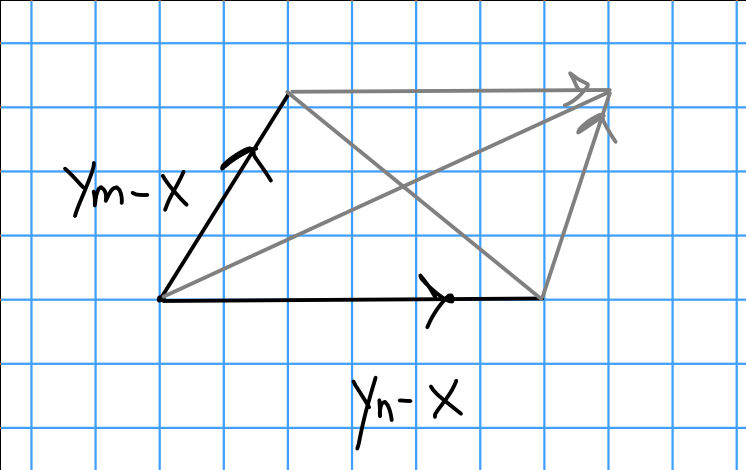
\includegraphics{figures/2019-11-12-11:25.png}\\

Then by the parallelogram theorem, we have
\begin{align*}
2(\norm{y_n - x}^2 + \norm{y_m - x}^2) = \norm{y_n - y_m}^2 + \norm{y_n + y_m - 2x}^2.
\end{align*}

which yields

\begin{align*}
\norm{y_n - y_m}^2 
&= 2 \norm{y_n - x}^2 + 2\norm{y_m - x}^2 - 4\norm{\frac 1 2 (y_n + y_m) - x}^2 \\
&\leq 2 \norm{y_n - x}^2 + 2\norm{y_m - x}^2 - 4\delta^2 \to 0,
\end{align*}

since \(\norm{y_n - x}_H \to 0\) since \(y_n \to_H x\).

It follows that \(\theset{y_n}\) is Cauchy in \(H\), so
\(y_n \mapsvia{H} y \in H\). But since the \(y_n\) were in \(M\) and
\(M\) is closed, we in fact have \(y\in M\). Since
\(\norm{x - y_n} \to \norm{x - y} = \delta\), we have the existence of
\(x\).

\begin{quote}
We'll establish uniqueness after part 2.
\end{quote}

\emph{Proof of Lemma (Part 2):}

Let \(u\in M\), we want to show that
\begin{align*}
\inner{z}{u} = \inner{x-y}{u} = 0
.\end{align*}

Without loss of generality, we can assume that \(\inner{z}{u} \in \RR\),
since \(u\) satisfies this property iff any complex scalar multiple
does.

Let \(f(t) = \norm{z + tu}^2\) where \(t\in \RR\). Then
\(f(t) = \norm{z}^2 + zt\inner{z}{y} = t^2 \norm{u}^2\).

We know that \(t\) attains a minimum at \(t=0\), since
\(z + tu = x - (y + u)\), but \(y\) was the closest element to \(x\) and
thus the norm is minimized exactly when \(z + tu = x - y \implies t=0\).

Because of this fact, we know that \(f'(0) = 0\). But by using Calculus,
we can compute that \(f'(0) = 2 \inner{z}{u}\), so \(\inner{z}{u}\) must
equal zero.

Now to show uniqueness, let \(y' \in M\) and suppose \(y' \neq u\) but
\(\norm{x-y'} = \delta\). Then \(x- y' = (x-y) + (y-y')\).

But these are two orthogonal terms, so we can apply Pythagoras to obtain

\begin{align*}
\norm{x-y'}^2 &= \norm{x-y}^2 + \norm{y-y'}^2 \\
\implies \delta &= \delta + c \\
\implies c &= 0 \\
\implies \norm{y-y'} &= 0 \\
\implies y &= y'
.\end{align*}

\begin{quote}
Note: the statement is the important thing here, less so this particular
proof.
\end{quote}

\hypertarget{trigonometric-series}{%
\subsection{Trigonometric Series}\label{trigonometric-series}}

\textbf{Theorem:} Let \(e_n(x) \definedas e^{2\pi i n x}\) for all
\(x\in [0, 1]\) and \(n\in \ZZ\). Then \(\theset{e_n}_{n\in \ZZ}\) is an
\emph{orthonormal basis} for \(L^2([0, 1])\).

\begin{quote}
Note: Orthonormality is easily check, so the crux of the proof is
showing it's a basis.
\end{quote}

\begin{quote}
Note: Elements in \(\mathrm{span}\theset{e_n}\) are referred to as
\emph{trigonometric polynomials}.
\end{quote}

Goal: We'll show that the span of the trigonometric polynomials are
dense in \(L^2([0, 1])\).

This will be a consequence of the following theorem:

\hypertarget{trigonometric-polynomials-are-dense-in-c00-1}{%
\subsubsection{\texorpdfstring{Trigonometric Polynomials are Dense in
\(C^0([0, 1])\)}{Trigonometric Polynomials are Dense in C\^{}0({[}0, 1{]})}}\label{trigonometric-polynomials-are-dense-in-c00-1}}

\textbf{Theorem (Periodic Analogue of the Weierstrass Approximation
Theorem):} If \(f\in C(\Pi)\) (where \(\Pi\) is a torus) and
\(\varepsilon > 0\), then there exists a trigonometric polynomial \(P\)
such that \(\abs{f(x) - P(x)} < \varepsilon\) uniformly for all
\(x\in \Pi\).

\begin{quote}
Note that this measures closes in the \emph{uniform} norm. We can relate
these by
\begin{align*}
\norm{f(x) -P(x)}_{L^2} \leq \norm{f(x) - P(x)}_{\infty} \text{, i.e. } \int_0^1 \abs{f(x) - P(x)}^2 \leq \sup_x \abs{f(x) - P(x)}^2
.\end{align*}
\end{quote}

\emph{Proof:} Identify \(\Pi = [- \frac 1 2, \frac 1 2)\). Suppose there
exists a sequence \(\theset{Q_k}\) of trigonometric polynomials such
that

\begin{align*}
Q_k(x) &\geq 0 \quad \text{ for all } x, k \\
\int_{-1/2}^{1/2} Q_k(x) ~dx &= 1 \quad \forall k \\
\forall \delta>0, \quad Q_k(x) &\mapsvia{u} 0 \text{ uniformly on } \Pi\setminus[-\delta, \delta]
.\end{align*}

\begin{quote}
Note that these properties are similar to what we wanted from
approximations to the identity.
\end{quote}

Define
\begin{align*}
P_k(x) = \int_{-1/2}^{1/2} f(y) Q_k(x - y) ~dy
\end{align*} by convolving over the circle, then \(P_k\) is also a
trigonometric polynomial.

We then have

\begin{align*}
I = \abs{ P_k(x) - f(x) } \leq 
\int_{-1/2}^{1/2} \abs{ f(x-y) - f(x) }
Q_k(y) ~dy \quad \text{by Property 2} 
.\end{align*}

We can now note that \(f\) is continuous on a compact set, so it is
uniformly continuous, and thus for \(y\) small enough, we can find a
\(\delta\) such that
\begin{align*}
\abs{f(x-y) - f(x)} < \varepsilon/2 \text{ for all } x \in B(\delta, x)
.\end{align*}

But this lets us break the integral into two pieces, \begin{align*}
I 
&\leq \int_{y \in B_\delta} \abs{ f(x-y) - f(x) }
Q_k(y) ~dy 
+ 
\int_{y \in B_\delta^c} \abs{ f(x-y) - f(x) }
Q_k(y) ~dy \\
&< \int_{y \in B_\delta} \frac \varepsilon 2~
Q_k(y) ~dy 
+
\int_{y \in B_\delta^c} \abs{ f(x-y) - f(x) }
Q_k(y) ~dy \\
&\leq \int_{y \in B_\delta} \frac \varepsilon 2~
Q_k(y) ~dy + \frac \varepsilon 2~ \quad \text{(for $k$ large enough)} \\
&\to 0 \quad \quad \text{since } Q_k \mapsvia{u} 0
.\end{align*}

\(\qed\)

\emph{Constructing \(Q_k\):}

Define
\begin{align*}
Q_k(x) = c_k \left( \frac {1 + \cos(2\pi x)}{2} \right)^k,
\end{align*}

where \(c_k\) is chosen to normalize the integral to 1 to satisfy
property 2. Property 1 is clear, so we just need to show 3,

Since \(\cos(x)\) is decreasing on \([\delta, \frac 1 2]\),
\begin{align*}
Q_k(x) \leq Q_k(\delta) = c_k \left( \frac{1 + \cos(2\pi \delta)}{2} \right)^k
.\end{align*}

Note that the numerator is less than 2, so the entire term is a constant
that is less than 1 being raised to the \(k\) power.

So this goes to zero exponentially, the question now depends on the
growth of \(c_k\). It turns out that \(c_k \leq (k+1)\pi\), so it only
grows linearly. So the whole quantity indeed goes to zero.

We can now write

\begin{align*}
1 &= 2c_k \int_0^{1/2} \left( \frac{1 + \cos(2\pi x)}{2} \right)^k dx \\
&= 2c_k \int_0^{1/2} \left( \frac{1 + \cos(2\pi x)}{2} \right)^k \sin(2\pi x) dx \\
&= \frac{2c_k}{\pi} 
\int_0^1 u^k ~du 
= 
\frac{2c_k}{\pi(k+1)}
.\end{align*}

\(\qed\)

\begin{quote}
Note: this is a nice proof!
\end{quote}

Question: when is a function equal to its Fourier series? We have
\(L^2\) convergence, but when do we get pointwise?

\textbf{Theorem from the 1960s:} any \(L^2\) function (in particular
continuous functions) converges to its Fourier series \emph{almost
everywhere}.

\hypertarget{thursday-november-14}{%
\section{Thursday November 14}\label{thursday-november-14}}

Let \(e_n(x) \definedas e^{2\pi i n x}\) for all \(n\in \ZZ\) and
\(x\in [0,1]\).

\textbf{Theorem:} \(\theset{e_n}_{n\in \ZZ}\) is an orthonormal basis
for \(L^2([0, 1])\).

\begin{quote}
Note that
\(L_2([0, 1]) = L^2(\Pi) = \theset{f\in L^2 \suchthat f(0) = f(1)}\),
since this only modifies a function at one point and we are identifying
functions that agree almost everywhere.
\end{quote}

\hypertarget{fourier-series}{%
\subsection{Fourier Series}\label{fourier-series}}

\textbf{Definition:} For any \(f\in L^1(\Pi)\), we define its
\emph{Fourier coefficients}
\begin{align*}
\hat{f}(n) \definedas \int_0^1 f(x) e^{-2\pi i n x} ~dx \quad \forall n \in \ZZ
\end{align*}

\begin{quote}
Note that this resembles \(\inner{f}{e_n}\), although this is not an
inner product space.
\end{quote}

\textbf{Definition:} The \emph{Fourier series} of \(f\) is defined as
\begin{align*}
\hat f(x) \definedas \sum_{n\in \ZZ} \hat{f}(n) e^{-2\pi i n x}
\end{align*}

\begin{quote}
Note that this isn't necessarily \emph{equal} to \(f\), this only makes
sense if the partial sums are converging to \(f\) in some sense.
\end{quote}

Define the \(N\)th partial sum
\begin{align*}
S_Nf(x) \definedas \sum_{\abs{n} \leq N} \hat{f}(n) e^{2\pi i n x}
.\end{align*}

\begin{quote}
Remark: We have \(L_2(\Pi) \subseteq L^1(\Pi)\), so the Fourier
coefficients \emph{do} make sense here as an inner product for all
\(f\in L_2(\Pi)\).
\end{quote}

\textbf{Some consequences:}

\begin{itemize}
\item
  By Riesz-Fischer, given any \(\theset{a_n} \in \ell^2(\ZZ)\), there is
  a function \(f\in L^2(\Pi)\) such that \(\hat{f}(n) = a_n\) for all
  \(n\).
\item
  By Parseval,
  \begin{align*}
  \sum_{n\in \ZZ} \abs{\hat{f}(n)}^2 = \int_0^1 \abs{f(x)}^2~dx
  \end{align*}
\item
  \(\lim_{N\to\infty} \norm{S_Nf - f}_2 = 0\), i.e.~the Fourier series
  of \(f\) converges to \(f\).
\end{itemize}

An answer: the Fourier series equals \(f\) in an \(L^2\) sense, but
recall that pointwise equality was a hard theorem proved only 50 or so
years ago!

\begin{quote}
Remark: note that for the Fourier transform, when \(f\in L^1\) and
\(\hat{f} \in L^1\), we have
\begin{align*}
f(x) = \int \hat{f} e^{-2\pi i x}~dx
,\end{align*} and we can get analogous statements here.
\end{quote}

\hypertarget{uniform-convergence-of-fourier-series}{%
\subsection{Uniform Convergence of Fourier
Series}\label{uniform-convergence-of-fourier-series}}

\textbf{Theorem:}

If \(f\in L^1(\Pi)\) and \(\theset{\hat{f}(n)} \in \ell^1\), then
\(S_Nf \mapsvia{u} f\) \emph{uniformly} on \(\Pi\).

\textbf{Corollaries:}

\begin{enumerate}
\def\labelenumi{\arabic{enumi}.}
\item
  If \(f\in C^1(\Pi)\), then \(S_N f \to f\) uniformly on \(\Pi\).
\item

  \begin{align*}
  f\in C(\Pi) \text{ and } f' \in L^2(\Pi) \implies S_Nf \mapsvia{u} f \text{ on } \Pi.
  \end{align*}

  \begin{quote}
  Note that the first condition alone is not sufficient: there exists a
  continuous function whose Fourier series diverges at a point.
  \end{quote}
\end{enumerate}

\emph{Proof:} Exercise

\begin{quote}
So if \(f\in C^1\), it is \emph{equal} to its Fourier series. Everyone
should know this fact!
\end{quote}

The following is a beautiful and fundamentally amazing fact:

\textbf{Fact (The Riemann-Localization Principle):}

If \(f\in L^1(\Pi)\) and \(f\) is constant on some neighborhood of
\(x \in \Pi\), then \(S_Nf(x) \to f(x)\) pointwise at this particular
\(x\).

\begin{quote}
Note that computing the Fourier coefficients requires integrating over
the entire circle, but somehow the behavior of the function elsewhere
doesn't matter at \(x\)!
\end{quote}

\emph{Proof of theorem:}

Since \(\theset{\hat{f}(n)} \in \ell^1(\ZZ)\), this gives us what we
need to apply the \(M\) test. So \(S_Nf \mapsvia{u} g\) uniformly for
some continuous \(g\).

How can we argue \(g = f\)? Consider

\begin{align*}
\hat{g}(n) 
&= \int_0^1 \left( \sum_{m\in \ZZ} \hat{f}(m) e^{2\pi i m x} \right) e^{-2\pi i n x} ~dx \\
&= \sum_{m\in \ZZ} \hat{f}(m) \int_0^1 e^{-2\pi i x (m-n)} \\
&= \sum_{m\in \ZZ} \hat{f}(m) \indic{m = n} \\
&= \hat{f}(m)
,\end{align*}

so the question is now whether
\begin{align*}
\hat{g}(n) = \hat{f}(n) ~\forall n \implies g = f \text{ almost everywhere }.
\end{align*}

\begin{quote}
Note: if we accept this fact at face value, this proof only requires
undergraduate analysis and uses facts about uniform convergence allowing
sums to commute with integrals.
\end{quote}

This will be true if \(f \in \ell^2\). Why is this the case?

It's not strict inclusion, since
\begin{align*}
L^2([0, 1]) \subseteq L^1([0, 1]) \text{ but } \ell^1(\ZZ) \not\subseteq \ell^2(\ZZ)
.\end{align*}

We can use the fact that if \(\sum \abs{f_n} < \infty\), then
\(f_n \to 0\), and in particular \(f_n\) is bounded. So we have

\begin{align*}
\left( \sum \abs{f_n}^2 \right)^{1/2} \leq \sum \abs{f_n} < \infty
.\end{align*}

But then since
\(\ell^1 \subseteq \ell^2 \implies \theset{\hat{f}(n)} \in \ell^2 \implies f\in L^2\)
by Riesz-Fischer and completeness.

\(\qed\)

\emph{An alternative proof: } Again suppose
\(\theset{\hat{f}(n)} \in \ell^1(\ZZ)\), \(S_Nf \to g\).

Since \(f\in L^2(\Pi)\) (because of the second assumption), we have
\(S_Nf \to f\) in \(L^2\).

\begin{quote}
Use the fact that \(f_n \to f \in L^2\) (or \(L^1\)) implies that a
\textbf{subsequence converges almost everywhere.}
\end{quote}

So \(f=g\) almost everywhere. \(\qed\)

\hypertarget{dual-of-a-vector-space}{%
\subsection{Dual of a Vector Space}\label{dual-of-a-vector-space}}

See notes on web page.

\begin{itemize}
\item
  Definition: Linear functional.
\item
  Examples.
\item
  Definition: Dual space.

  \begin{itemize}
  \tightlist
  \item
    Don't need \(X\) to be complete, just need a normed vector space.
  \end{itemize}
\item
  Theorem: A linear functional is continuous iff it is \emph{bounded}.
\item
  Definition: Bounded functional.

  \begin{itemize}
  \tightlist
  \item
    Can't define as \(\abs{L(x)} \leq C\) (since linearity allows
    pulling out scalars), so we can just restrict attention to
    \(\theset{x\suchthat \norm{x} \leq 1}\).
  \end{itemize}
\item
  \(X\dual\) is always a vector space
\item
  \(X\dual\) is always a Banach space with norm
  \(L \mapsto \sup_{x\in X} \abs{L(x)}\).
\item
  \(y \mapsto L_y \definedas \inner{\wait}{y}\) is a conjugate linear
  isometry \(H \to H\dual\) which is surjective.
\item
  Riesz Representation Theorem (for Hilbert spaces)

  \begin{itemize}
  \tightlist
  \item
    Use the fact that \(L\in H\dual \implies \ker L\) is a closed
    subspace.
  \item
    \(z\in M^\perp\), look at \(\inner{ (Lx)z - (Lz)x }{z}\).
  \end{itemize}
\end{itemize}

Upcoming:

\begin{itemize}
\item
  A bit about \(L^p\) spaces
\item
  Dual of \(L^1\), dual of \(L^\infty\).
\item
  Abstract measure theory
\item
  Hahn-Banach, Radon-Nikodym, and Lebesgue Density from the perspective
  of differentiation theorems.
\end{itemize}

\hypertarget{tuesday-november-19}{%
\section{Tuesday November 19}\label{tuesday-november-19}}

\hypertarget{lp-spaces}{%
\subsection{Lp Spaces}\label{lp-spaces}}

Given \(f:\RR^n \to \CC\) and \(0 < p < \infty\), we define
\begin{align*}
\norm{f}_p = \left( \int \abs{f}^p \right)^{1/p}.
\end{align*}

and \(L^p(\RR^n) = \theset{f \suchthat \norm{f}_p \infty }\).

We also define
\begin{align*}
\norm{f}_\infty = \inf_{a \geq 0} \theset{ m(\theset{x \suchthat f(x) > a}) = 0 }
\end{align*}

which is morally the ``best upper bound almost everywhere''.

\begin{quote}
\textbf{Qual problem alert}: If \(X \subseteq \RR^n\) with
\(\mu(X) < \infty\) then \(\norm{f}_p \to \norm{f}_\infty\).
\end{quote}

Note that \(\abs{f(x)} \leq \norm{f}_\infty\) almost everywhere, and if
\(\abs{f(x)} \leq M\) almost everywhere, then
\(\norm{f}_\infty \leq M\).

For \(1 \leq p \leq \infty\), \(( L^p, \norm{\wait}_p)\) yields a
complete normed vector space. Scaling and non-degeneracy are fairly
clear, it just remains to show the triangle inequality (sometimes
referred to as Minkowski's inequality), i.e.~
\begin{align*}
f, g\in L^p \implies \norm{f+g}_p \leq \norm{f}_p + \norm{g}_p.
\end{align*} For \(p=2\), this boiled down to Cauchy-Schwarz, here we'll
need a souped-up version.

\textbf{Definition:} If \(1 \leq p \leq \infty\), we define the
\emph{conjugate exponent} of \(p\) as the \(q\) satisfying
\(\frac 1 p + \frac 1 q = 1\).

An immediate consequence is that
\begin{align*}
q = \frac{p}{p-1}
.\end{align*}

\textbf{Holder's Inequality:} If \(f, g\) are measurable functions then
\begin{align*}
\norm{fg}_1 \leq \norm{f}_p \norm{g}_q.
\end{align*}

\emph{Proof of Minkowski:}

\begin{align*}
\abs{f + g}^p 
&= \abs{f+g} \abs{f+g}^{p-1} \\
&\leq ( \abs{f} + \abs{g} ) \abs{f+g}^{p-1} \\
&\implies \int \abs{f+g}^p \leq \int \abs{f} \abs{f+g}^{p-1} + \int \abs{g} \abs{f + g}^{p-1} \\
&\leq \norm{f}_p ( \int \abs{f+g}^{(p-1)q}  )^{1/q}
+ \norm{g}_p ( \int \abs{f+g}^{(p-1)q}  )^{1/q} \\
&= (\norm{f}_p + \norm{g}_p) + ( \int\abs{f+g}^p )^{1 - 1/p} \\
&= (\norm{f}_p + \norm{g}_p) + ( \int\abs{f+g}^p )^{1/q}
,\end{align*}

and taking \(p\)th roots yields the result. (?? Revisit) \(\qed\)

\begin{quote}
Note: For \(1\leq p \leq \infty\), \(L^p\) is a Banach space.
\end{quote}

\begin{quote}
AM-GM: \(\sqrt{ab} \leq \frac{a+b}{2}\).
\end{quote}

\emph{Proof of Holder:}

We'll use the following key fact:
\begin{align*}
a^\lambda b^{1-\lambda} \leq \lambda a + (1-\lambda)b
\end{align*}

with equality iff \(a=b\). This can be verified by the first derivative
test.

\textbf{Important simplfication:} we can assume that
\(\norm{f}_p = \norm{g}_q = 1\), since
\begin{align*}
\norm{fg}_1 \leq \norm{f}_p \norm{f}_q \iff \int \frac{\abs{f}}{\norm{f}_p} \frac{\abs{g}}{\norm{g}_q}
.\end{align*}

Applying the key fact, we can choose
\(\lambda = \frac 1 p, a =\abs{f}^p, b = \abs{g}^q\).

We then obtain
\begin{align*}
\int \abs{f} \abs{g} \leq \int \frac{\abs{f}^p}{p} \frac{\abs{g}^q}{q} = \frac 1 p + \frac 1 q = 1.
\end{align*} \(\qed\)

\hypertarget{dual-of-lp}{%
\subsection{\texorpdfstring{Dual of
\(L^p\)}{Dual of L\^{}p}}\label{dual-of-lp}}

Given \(g\in L^q\), define an operation

\begin{align*}
\Lambda_g(f): L^p \to \CC \\
f \mapsto \int f g
.\end{align*}

Note that this makes sense by Holder's inequality, i.e.~\(fg\) is
integrable. This defines a linear functional on \(L^p\), which is
continuous by Holder, since we have
\begin{align*}
\abs{\Lambda_g(f)} \leq \norm{g}_q \norm{f}_p
\end{align*} where \(\norm{g}_q\) is a constant that works for all
\(f \in L^p\).

\begin{quote}
Recall: linear functionals are continuous iff bounded.
\end{quote}

We have
\begin{align*}
\norm{\Lambda_g}_{(L^p)\dual} \definedas \sup_{\norm{f}_p = 1} \abs{\int fg} \leq \norm{g}_q
.\end{align*}

\begin{quote}
In fact, we have equality here for every \(g\in L^q\). This is sometimes
referred to as the converse of Holder.
\end{quote}

Thus the map \(g \mapsto \Lambda_g\) is an \emph{isometric} map
\(L^q \injects (L^p)\dual\) for \(1 \leq p,q \leq \infty\).

By Riesz representation, it turns out that this is a surjection as well
for \(p\neq \infty\).

\textbf{Big Fact}: This breaks for \(p=\infty\), but for
\(1 \leq p < \infty\), this mapping is surjective.

\hypertarget{riesz-representation}{%
\subsection{Riesz Representation}\label{riesz-representation}}

\textbf{Theorem (Riesz Representation):} Suppose \(1\leq p < \infty\)
and let \(q\) be its conjugate exponent, and let \(X\subseteq \RR^n\) be
measurable.

Given any \(\Lambda \in (L^p(X))\dual\), there exists a unique
\(g\in L^q(X)\) such that for all \(f\in L^p(X)\), we have
\begin{align*}
\Lambda(f) = \int_X fg
\quad \text{ and } \quad 
\norm{\Lambda}_{(L^p(X))\dual} = \norm{g}_{L^q(X)}
.\end{align*}

\textbf{Summary:}

\begin{itemize}
\tightlist
\item
  If \(1\leq p < \infty\), we have \((L^p)\dual = L^q\).
\item
  \((L^\infty)\dual \supset L^1\), since the isometric mapping is always
  injective, but \emph{never} surjective, so this containment is always
  proper (requires Hahn-Banach Theorem).
\end{itemize}

\begin{quote}
For qual, supposed to know this for \(p=1\). \(p=2\) case is easy by
Riesz Representation for Hilbert spaces.
\end{quote}

\emph{Proof (in the special case where \(1\leq p < 2\) and
\(m(X) < \infty\)):}

We'll use the fact that we know this for \(p=2\) already.

Let \(\Lambda \in (L^p)\dual\), then we know
\begin{align*}
\abs{\Lambda(f)} \leq \norm{\Lambda}_{(L^p)\dual} \norm{f}_p
,\end{align*} since \(\norm{\Lambda}\) is the \emph{best} upper bound.

\begin{quote}
Note: in general, there are no inclusions between \(L_p, L_q\), but
restricting to a compact set changes this fact. Example from homework:
\begin{align*}
L^2(X) \subseteq L^1(X) \text{ for } m(X) < \infty
.\end{align*}
\end{quote}

\begin{quote}
This follows from
\begin{align*}\norm{f}_1 \leq \norm{f}_2 \norm{1}_2 = m(X)^{1/2} \norm{f}
.\end{align*} But this works for \(L^2(X) \subseteq L^p(X)\) by taking
\begin{align*}
\norm{f}_p^p = \int \abs{f}^p \leq ( \int \abs{f}^2 )^{p/2} (\int \abs{1}^{?})^{1 - \frac 2 p}
\end{align*} by Holder with \(\frac 2 p\).
\end{quote}

So we can write
\begin{align*}
\abs{\Lambda(f)} = \norm{\Lambda} m(X)^{\frac 1 p - \frac 1 2} \norm{f}_2 \quad \forall f\in L^2,
\end{align*}

which verifies that \(\Lambda\) is a continuous linear functional on
\(L^2\), so \(\Lambda \in (L^2)\dual\), and by Riesz Representation,
\(\exists g \in L^2\) such that \(\Lambda(f) = \int fg\) for all
\(f\in L^2\).

This is almost what we want, but we need \(g\in L^q\) and \(f\in L^p\).
We also want to show that \(\norm{\Lambda} = \norm{g}_q\).

\textbf{Claim}: \(g\in L^q\) and \(\norm{g}_q \leq \norm{\Lambda}\).

\begin{quote}
Pause on the proof, we'll come back to it!
\end{quote}

Note that since \(L_2 \subseteq L^p\) and both have simple functions as
a dense subset, \(L^2\) is in fact dense in \(L^p\).

So let \(f \in L^p\) and pick a sequence \(f_n \subset L^2\) converging
to \(f\) in the \(L^p\) norm.

Then \(\Lambda(f_n) \to \Lambda(f)\) by continuity, and since
\(g\in L^q\), integrating against \(g\) is a linear functional
\(\Lambda_q (f_n)\) on \(L^q\) converging to \(\int f g\), so
\(\Lambda(f) = \int fg\). \(\qed\)

\begin{quote}
Definitely need to know: \((L^1)\dual = L^\infty\)!
\end{quote}

\emph{Proof of claim:} Suppose it's not true, so
\(\norm{g}_\infty > \norm{\Lambda}_{(L^1)\dual}\).

Using the fact that \(\norm{g}\) is the best lower bound, there must be
a positive measure set such that \(\abs{g(x)} \geq \norm{\Lambda}\). So
there is some set
\(E = \theset{x \suchthat \abs{g(x) > \norm{\Lambda}}}\) with
\(m(E) > 0\).

Let
\begin{align*}
h = \frac{\overline{g}}{\abs{g}} \frac{\chi_E}{m(E)}
.\end{align*}

\begin{quote}
Note: useful technique!
\end{quote}

Then \(h\in L^2\) and \(\norm{h} = 1\).

Then
\begin{align*}
\Lambda(h) = \frac{1}{m(E)} \int_E \abs{g} \geq \norm{\Lambda} O(1)
,\end{align*} which is a contradiction.

\hypertarget{thursday-november-21}{%
\section{Thursday November 21}\label{thursday-november-21}}

\hypertarget{abstract-measure-theory}{%
\subsection{Abstract Measure Theory}\label{abstract-measure-theory}}

\textbf{Definition}: Let \(X\) be a set and \(\mathcal M\) be a
\(\sigma\dash\)algebra of subsets of \(X\).

Then \((X, \mathcal M)\) is referred to as a \emph{measurable} space,
noting that we have not yet equipped it with a measure \(\mu\).

\textbf{Definition:} A \emph{measure} \(\mu\) on \((X, \mathcal M)\) is
a function \(\mu: \mathcal M \to [0, \infty]\) such that

\begin{itemize}
\item
  The silly condition, \(\mu(\emptyset) = 0\)
\item
  The important condition,
  \(\mu(\disjoint_{i\in \NN} E_i) = \sum_{i\in\NN} \mu(E_i)\).
\end{itemize}

Then \((X, \mathcal M, \mu)\) is called a \emph{measure space}. Things
can be measured in this setting, but more importantly, an integral can
be defined.

\textbf{Definition:} A measure is \emph{\(\sigma\dash\)finite} iff
\(X = \union E_j\) with \(m(E_j) < \infty\) for each \(j\).

\begin{quote}
Note: most measures encountered in practice seem to be
\(\sigma\dash\)finite, so we could just as well incorporate this into
our definition.
\end{quote}

\emph{Examples:}

\begin{itemize}
\item
  The Lebesgue measure
\item
  Let \(X = \theset{x_n}_{n=1}^\infty\) a countable collection of
  objects, \(\theset{\mu_n \in [0,\infty]}\), and define
  \(\mu(x_n) \definedas \mu_n\).

  Then we can take the \(\sigma\dash\)algebra
  \(\mathcal M = \mathcal P(X)\), so

  \begin{align*}
  \mu: \mathcal P(X) \to [0, \infty] \\
  E \mapsto \sum_{\theset{n \mid~ x_n \in E}} \mu_n
  .\end{align*}

  In the special case \(\mu_n = 1\) for all \(n\), we have
  \(\mu(E) = \# E\), the number of elements in \(E\), which is the
  counting measure.
\item
  Let \(X = \RR^n\) and let \(\mathcal M\) be the Lebesgue measurable
  subsets, and let \(\mu(E) = \int_E f\) for some fixed \(f \in L^+\).

  \begin{quote}
  Exercise: Show that this defines a measure.
  \end{quote}

  In the special case \(f \equiv 1\), we get the usual Lebesgue measure
  \(\mu = m\). We write \(d\mu \definedas f dx\). Note that
  \begin{align*}
  m(E) = 0 \iff \mu(E) = 0
  ,\end{align*} which is referred to as \emph{absolute continuity}.

  \begin{quote}
  Note that all absolutely continuous measures occur in this way! But
  there are more exotic measures. Thinking about representability
  theorems, this says that measures are like ``generalized integrable
  functions'', but the collection of measures is richer.
  \end{quote}
\item
  The Dirac mass:
  \begin{align*}
  \delta_0(E) = \begin{cases} 1 & 0\in E \\ 0 & \text{else}
  \end{cases}.\end{align*}
\end{itemize}

\hypertarget{basic-properties-of-measures}{%
\subsection{Basic Properties of
Measures}\label{basic-properties-of-measures}}

Fix a measure space \((X, \mathcal M, \mu)\).

\begin{enumerate}
\def\labelenumi{\arabic{enumi}.}
\item
  \textbf{Monotonicity}:
  \begin{align*}
  E_1 \subseteq E_2 \implies \mu(E_1) \leq \mu(E_2)
  .\end{align*} This follows from writing
  \begin{align*}
    E_2 = E_1 \disjoint (E_2 \setminus E_1)
    \end{align*} and taking measures, which are always \(\geq 0\).
\item
  \textbf{Subadditivity}:
  \begin{align*}
  \mu(\union E_i) \leq \sum \mu(E_i)
  \end{align*}
\item
  \textbf{Continuity from above and below:} \begin{align*}
  E_j \nearrow E &\implies \mu(E_j) \to \mu(E) \text{ and }  \\ E_j \searrow E, ~~\mu(E_1) < \infty &\implies \mu(E_j) \to \mu(E)
  .\end{align*}
\end{enumerate}

\textbf{Definition:} A measure space is \emph{complete} iff when
\(F \in \mathcal M\) is measurable, \(\mu(F) = 0\), and
\(E\subseteq F\), we have \(E \in \mathcal M\).

\begin{quote}
Recall that the Lebesgue measure is complete, and the Borel measure is
\emph{not}. Review why this is the case!
\end{quote}

\hypertarget{construction-of-measures}{%
\subsection{Construction of Measures}\label{construction-of-measures}}

Given an \((X, \mathcal M)\), we construct \(\mu\) in the following way:

\begin{enumerate}
\def\labelenumi{\arabic{enumi}.}
\tightlist
\item
  Define an outer measure (or premeasure) \(\mu^*\) on
  \(\mathcal P(X)\).
\item
  Caratheodory:
  \begin{align*}
  E\subseteq X \text{ is measurable } \iff \mu_*(A) = \mu_*(A\intersect E) + \mu_*(A\intersect E^c) \quad \forall A \subseteq X
  .\end{align*}
\end{enumerate}

\begin{quote}
Note: it is worth recalling why this is equivalent to the usual ``open
set'' definition, i.e.~\(\exists G\) open such that
\(\mu_*(G\setminus E < \varepsilon\), where we really needed a topology
to talk about open sets.
\end{quote}

\begin{enumerate}
\def\labelenumi{\arabic{enumi}.}
\setcounter{enumi}{2}
\tightlist
\item
  Defining
  \begin{align*}
  \mathcal M \definedas \theset{\text{Caratheodory measurable sets}}
  \end{align*} yields a \(\sigma\dash\)algebra and
  \(\restrictionof{\mu_*}{\mathcal M}\) is a measure.
\end{enumerate}

\hypertarget{measurable-functions}{%
\subsection{Measurable Functions}\label{measurable-functions}}

Next up: define integrability, by first defining what it means for a
function to be measurable.

\textbf{Definition:} A function \(f: X \to \overline{\RR}\) is
\emph{measurable} \(\iff\)
\(\mu(\theset{x\in X \suchthat f(x) > a}) \in \mathcal M\) for all
\(a\in \RR\).

We say two functions are \emph{equal almost everywhere} if they disagree
on a measure zero set, and we can define simple functions in a similar
way.

\textbf{Definition:} If \(\phi\) is simple,
i.e.~\(\phi = \sum_{j=1}^N a_j \chi_{E_j} \in L^+\) (is non-negative),
then
\begin{align*}
\int \phi ~d\mu \definedas \sum_j a_j \mu(E_j)
.\end{align*}

Then if \(f\in L^+\), we define
\begin{align*}
\int f d\mu = \sup \theset{\int \phi ~d\mu \suchthat 0\leq \phi \leq f, \phi\text{ is simple. }}
.\end{align*}

For \(f\) arbitrary and measurable, write \(f = f_+ - f_-\), and define
\begin{align*}
\int f d\mu \definedas \int f_+ d\mu - \int f_- d\mu
\end{align*} whenever it makes sense (i.e.~both are not infinite)

Consider an earlier example: given \((X, \mathcal M, \mu)\) and
\(f\in L^+(X, \mu)\), we can define
\begin{align*}
\mu_f(E) \definedas \int_E f d\mu \in \overline{\RR}
.\end{align*}

This always yields a measure, and moreover has the property
\(\mu(E) = 0 \implies \mu_f(E) = 0\).

\begin{quote}
Note that we can actually generalize and let \(f\in L^+\). Then the
measure defined here can take on negative or even complex numbers, which
turns out to be a useful (see ``\emph{signed measures}'').
\end{quote}

This is closely related to the usual notion of signed area between a
curve and the \(x\dash\)axis we deal with in Calculus.

\hypertarget{absolute-continuity-and-radon-nikodym}{%
\subsection{Absolute Continuity and
Radon-Nikodym}\label{absolute-continuity-and-radon-nikodym}}

\textbf{Definition} Let \(\mu, \nu\) be two measures on
\((X, \mathcal M)\). Then we say \(\nu \ll \mu \iff \nu(E) = 0\)
whenever \(E\in\mathcal M\) and \(\mu(E) = 0\), and that \emph{\(\nu\)
is }absolutely continuous with respect to \(\mu\)*.

\emph{Exercise:} If \(\nu\) is finite, i.e.~\(\nu(X) < \infty\), then
\begin{align*}
\nu \ll \mu \iff \forall\varepsilon >0~ \exists\delta > 0 ~ \suchthat \mu(E) < \delta\implies \nu(E) < \varepsilon
,\end{align*} which explains the terminology.

\begin{quote}
Worth looking at more in-depth. Should be in textbook.
\end{quote}

\textbf{Theorem (Partial Radon-Nikodym):} If \(\mu, \nu\) are two
\(\sigma\dash\)finite measures on \((X, \mathcal M)\) such that
\(\nu \ll \mu\), then there exists a unique non-negative function
\(f\in L^1(X, \mu)\) such that
\begin{align*}
d\nu = f d\mu
\text{ and }
\nu(E) = \int_E f d\mu \text{ for all } E\in \mathcal M
.\end{align*}

\begin{quote}
Note: this is a representation theorem. This somehow all traces back to
the Riesz Representation theorem for Hilbert spaces, which was a trivial
proof! Worth recalling.
\end{quote}

\emph{Proof (Sketch)}: We can assume \(\mu, \nu\) are
\(\sigma\dash\)finite (there are standard techniques to do this).

Now define the measure \(\rho: \nu + \mu\) and
\(L(\psi) = \int_X \psi d\nu\) for all \(\psi \in L^2(X, \rho)\). Then
\(L\) turns out to be a \emph{continuous} linear functional on
\(L^2(X, \rho)\), which isn't completely obvious. This follows because
it is bounded, since for all \(\psi \in L^2(\rho)\) we have

\begin{align*}
\int \abs{\psi} d\nu 
&\leq \int \abs{\psi} d\rho \\
&\leq \norm{\psi}_{L^2(\rho)} \rho(X)^{1/2} \\
&\leq C \norm{\psi}_{L^2(\rho)}
,\end{align*}

which follows from an application of Cauchy-Schwarz.

Then there exists a \(g\in L^1(\rho)\) such that
\begin{align*}
\int \psi d\nu = \int \psi g d\rho = \int \psi g d\nu + \int \psi g d\mu
.\end{align*}

By collecting terms, we obtain
\begin{align*}
\int_X \psi(1-g) d\nu = \int_X \psi g d\mu \quad \forall \psi\in L^2(\rho).
\end{align*}

Now consider letting \(\psi = \chi_E\) for some set. Then
\(\nu(E) = \int_E g d\rho\), from which it can be deduced that
\(0\leq g \leq 1\) almost everywhere.

Since \(\nu \ll \mu\), we actually have \(0\leq g < 1~ \rho\dash\)a.e.
instead. This follows from taking \(B = \theset{g(x) = 1}\) and
\(\psi = \chi_B\) and using the above identity we found to deduce that
\(\mu(B) = 0\) and thus \(\nu(B) = 0\) and \(\rho(B) = 0\).

Now let
\begin{align*}
\psi = \chi_E(1 ) g + g^2 + \cdots g^n)
,\end{align*}

yielding

\begin{align*}
\int_E (1-g^{n+1}) d\nu &= \int_E (1 + g + \cdots + g^n) d\mu \\
\to_{DCT} \nu(E) &= \int_E \frac{g}{1-g} d\mu
,\end{align*}

so we can take the integrand on the RHS to be our \(f\).

\(\qed\)

\begin{quote}
Beautiful proof! Due to Von Neumann.
\end{quote}

To show: the fundamental theorem of Calculus for measures, i.e.~the
Lebesgue differentiation theorem, which looks like
\begin{align*}
\lim_{r\to 0} \frac{1}{m(B_r(x))} \int_{B_r(x)} f(y) ~dy = f(x) ~\text{ a.e. }
\end{align*} and specializes when \(f = \chi_E\).

\hypertarget{tuesday-november-26th}{%
\section{Tuesday November 26th}\label{tuesday-november-26th}}

\hypertarget{differentiation}{%
\subsection{Differentiation}\label{differentiation}}

\emph{Question:} Let \(f\in L^1([a, b])\) and
\(F(x) = \int_a^x f(y) ~dy\). Is \(F\) differentiable a.e. and
\(F' = f\)?

If \(f\) is continuous, then absolutely yes.

Otherwise, we are considering
\begin{align*}
\frac{f(x+h) - F(x)}{h} = \frac{1}{h} \int_x^{x+h} f(y)~dy \to_? f(x)
\end{align*}

so the more general question is
\begin{align*}
\lim_{\substack{m(I) \to 0 \\  x\in I}} \frac{1}{m(I)} \int_I f(y) ~dy =_? f(x) ~\text{a.e.}
\end{align*}

Note that if \(f\) is continuous, since \([a, b]\) is compact, we have
uniform continuity and
\begin{align*}
\frac{1}{m(I)} \int_I f(y) - f(x) ~dy < \frac{1}{m(I)} \int_I \varepsilon \to 0
.\end{align*}

\hypertarget{lebesgue-differentiation-and-density-theorems}{%
\subsection{Lebesgue Differentiation and Density
Theorems}\label{lebesgue-differentiation-and-density-theorems}}

\textbf{Theorem:} If \(f\in L^1(\RR^n)\) then
\begin{align*}
\lim_{\substack{m(B) \to 0 \\ x\in B}} \int \frac{1}{m(B)} \int_B f(y)~dy = f(x) ~\text{a.e.}
\end{align*}

\begin{quote}
Note: although it's not obvious at first glance, this really is a
theorem about differentiation.
\end{quote}

\textbf{Corollary (Lebesgue Density Theorem):} For any measurable set
\(E \subseteq \RR^n\), we have
\begin{align*}
\lim_{r\to 0} \frac{m(E\intersect B_r(x))}{m(B_r(x))} = 1 ~a.e.
\end{align*}

\emph{Proof:} Let \(f = \chi_E\) in the theorem.

We want to show
\begin{align*}
Df(x) \definedas \limsup_{\substack{m(B) \to 0 \\ x\in B}} \abs{\frac{1}{m(B)} \int_B (f(y) - f(x))~dy  } \to 0
\end{align*}

Note that we can replace \(\limsup \cdots\) with
\begin{align*}
\lim_{\varepsilon \to 0} \sup_{\substack{0\leq m(B) \leq \varepsilon \\ x\in B}} \cdots
,\end{align*}

which is well defined as it is a decreasing sequence of numbers bounded
below by zero.

Next we'll introduce that \emph{Hardy-Littlewood Maximal Function},
given by
\begin{align*}
Mf(x) \definedas \sup_{x\in B} \frac{1}{m(B)} \int_B \abs{f(y)} ~dy
\end{align*}

\begin{quote}
\emph{Exercise}: show that \(Mf\) is a measurable function. (Hint: it's
easy to show that the appropriate preimage is open.)
\end{quote}

\textbf{Theorem (Hardy-Littlewood Maximal Function Theorem):} Let
\(f\in L^1(\RR^n)\), then
\begin{align*}
m({ x\in \RR^n \suchthat Mf(x) > \alpha  }) \leq \frac{3^n}{\alpha} \norm{f}_1.
\end{align*}

\begin{quote}
Idea: if you look at all balls intersecting a given ball of radius
\(\alpha\), the worst case is that the other ball doesn't intersect and
is of the same radius. But then you can draw a ball of radius
\(3\alpha\) and cover every such intersecting ball.
\end{quote}

\begin{quote}
Exercise: As a corollary, \(Mf(x) < \infty~a.e.\)
\end{quote}

This is called a \emph{weak type} estimate, compared to a strong type
\(\norm{Mf}_1 \leq C \norm{f}_1\). Note that by Chebyshev, a strong
estimate would imply the weak one because
\begin{align*}
m(\theset{x \suchthat mf(x) > \alpha}) \leq \frac{1}{\alpha} \norm{Mf}_1 \not\leq \frac{C}{\alpha} \norm{f}_1,
\end{align*}

which is an inequality that doesn't hold (hence the theorem) because
there is an \(L^1\) function for which \(Mf\) is \emph{not} \(L^1\).

\emph{Proof of differentiation theorem:} The goal is to show
\(Df(x) = 0\) a.e.

We will show that \(m(\theset{x\suchthat Df(x) > \alpha}) = 0\) for all
\(\alpha > 0\).

\textbf{Some facts:}

\begin{enumerate}
\def\labelenumi{\arabic{enumi}.}
\item
  If \(g\) is continuous, then \(Dg(x) = 0\) a.e. by uniform
  convergence.
\item

  \begin{align*}
  D(f_1 + f_2)(x) \leq Df_1(x) + Df_2(x)
  \end{align*} by applying the triangle inequality and distributing the
  \(\limsup\).
\item

  \begin{align*}
  Df(x) \leq Mf(x) + \abs{f(x)}
  \end{align*}
\end{enumerate}

Fix an \(\alpha\) and fix an \(\varepsilon\). Choose a continuous \(g\)
such that \(\norm{f-g}_1 < \varepsilon\).

Writing \(f=f-g+g\), we have

\begin{align*}
Df(x) 
&\leq D(f-g)(x) + Dg(x) \\
&=D(f-g)(x) + 0 \\
&\leq M(f-g)(x) + \abs{(f-g)(x)}.
,\end{align*}

Then
\begin{align*}
Df(x) \geq \alpha \implies M(f-g)(x) \geq \frac{\alpha}{2}
\end{align*} or
\begin{align*}
\abs{(f-g)(x)} \geq \frac{\alpha}{2}
.\end{align*}

So we have
\begin{align*}
\theset{x\suchthat Df(x) > \alpha} \subseteq \theset{x\suchthat M(f-g)(x) > \frac\alpha 2} \union \theset{x\suchthat \abs{f(x) - g(x)} > \frac\alpha 2}
.\end{align*} Applying measures turns this into an inequality.

But then applying the maximal function theorem, we have

\begin{align*}
m(\theset{x\suchthat Df(x) > \alpha}) 
&\leq \frac{3^n}{\alpha/2} \norm{f-g}_1 + \frac 2 \alpha \norm{f-g}_1 \\
&\leq \varepsilon \left(\frac{2(3^n + 1)}{\alpha} \right)
.\end{align*}

\(\qed\)

\begin{quote}
Note that somehow proving the maximal function theorem here really paved
the way, and allows some generalization. Here we computed an average
over a solid ball, but there is a notion of surface measure, so we can
consider averaging over the surface of spheres, which can include more
exotic objects like spheres in \(\ZZ^d\).
\end{quote}

\emph{Proof of HL Maximal Function Theorem:} Let
\begin{align*}
E_\alpha \definedas \theset{x\suchthat Mf(x) > \alpha}
.\end{align*}

If \(x\in E_\alpha\), then it follows that there is a \(B_x\) such that
\begin{align*}
\frac{1}{m(B_x)} \int_{B_x} \abs{f(y)} ~dy > \alpha \iff m(B_x) < \frac 1 \alpha \int_{B_x} \abs{f(y)} ~dy
.\end{align*}

Note that if \(E_\alpha\) were compact, there would only be finitely
many such balls, so let \(K \subseteq E_\alpha\) be a compact subset. We
will be done if we can show that
\begin{align*}
m(K) < \frac{3^n}{\alpha} \norm{f}_1
,\end{align*} since we can always find a compact \(K\) such that
\(m(E_\alpha\setminus K)\) is small.

There exists a finite collection \(\theset{B_k}^N\) such that each
\(B_k = B_x\) for some \(x\in E_\alpha\), \(K \subseteq \union B_k\),
and
\begin{align*}
m(B_k) \leq \frac{1}{\alpha} \int_{B_k} \abs{f(y)}~dy
.\end{align*}

Supposing that the \(B_k\) were disjoint (which they are not!), then we
would be done since

\begin{align*}
m(K) 
&\leq \sum m(B_k) \\
&\leq \frac{1}{\alpha} \sum \int_{B_k} \abs{f(y)} ~dy \\
&\leq \frac{1}{\alpha} \int_{\RR^n} \abs{f(y)}
.\end{align*}

\emph{Lemma (The Vitali Covering Lemma):} Given any collection of balls
\(B_1, \cdots, B_N\), there exists a sub-collection \(A_1, \cdots, A_M\)
which are disjoint with
\begin{align*}
m(\union^N B_k) \leq 3^n \sum^M m(A_j)
.\end{align*}

\begin{quote}
Note that this follows directly from picking the largest ball first,
then picking further balls that avoid everything already picked and are
chosen in decreasing order of size. The \(3^n\) factor comes from the
earlier fact that tripling the radius covers everything you didn't pick.
\end{quote}

But now we can replace \(B_k\) with such a sub-collection \(A_k\) in the
above set of inequalities, which proves the theorem. \(\qed\).

\hypertarget{tuesday-december-3rd}{%
\section{Tuesday December 3rd}\label{tuesday-december-3rd}}

\textbf{Lebesgue Differentiation Theorem:} If \(f\in L_{loc}(\RR^n)\),
then
\begin{align*}
\lim_{m(B) \to 0; x\in B} \frac 1 {m(B)} \int_B f(y) ~dy = f(x) \quad \text{for almost every $x$}
\end{align*}

\hypertarget{rademacher-functions}{%
\subsection{Rademacher Functions}\label{rademacher-functions}}

\emph{Definition:} The \emph{Rademacher functions} are given by
functions \(r_n: [0, 1] \to \theset{-1, 1}\):

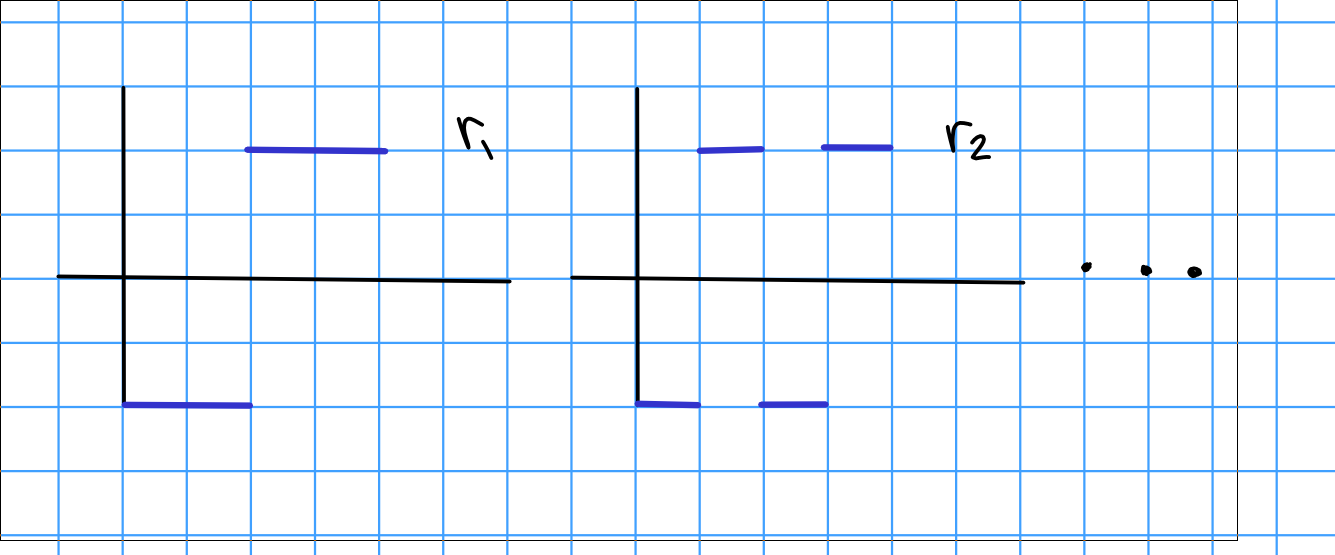
\includegraphics{figures/2019-12-03-11:11.png}\\

Note the self-similar nature: \(r_2\) just does \(r_1\) on each
half-interval. Now lift these to \(\RR^n\) by taking products.

\emph{Facts:}

\(\theset{r_n}\) forms an orthonormal system in \(L^2([0, 1])\), and

\begin{align*}
\int_0^1 r_n(x) ~dx &= 0 \\
\int_0^1 r_n(x) r_m(x) ~dx &= 0 \quad \text{ if } n\neq m \\
\int_0^1 r_n(x)^2 ~dx &= 1 \quad \forall n
.\end{align*}

\begin{quote}
Think of these as modeling a random process, like coin flips.
\end{quote}

Consider
\begin{align*}
a_n(t) \definedas \frac{1}{2}(r_n(t) + 1)
,\end{align*} which essentially sends \(-1 \to 0\) and \(1\to 1\) in
each \(r_n\).

Note that when \(t = \frac 1 4\), we have
\(\theset{a_n(t)} = [0, 0, 1, 1, 1, \cdots]\), which is the binary
expansion of \(t\).

If we define \(S_N(t) = \sum_{n=1}^N r_n(t)\), we have
\(\int_0^1 S_N(t) = 0\) and \(\int_0^1 S_N(t)^2 = n\), which says that
the expected value is zero (as many heads as tails) and the variance is
additive.

\hypertarget{law-of-large-numbers}{%
\subsection{Law of Large Numbers}\label{law-of-large-numbers}}

\textbf{Strong Law of Large Numbers:}
\begin{align*}
\frac{S_N(t)}{N} \to 0 \text{ as } N\to \infty \text{ for almost every } t\in [0, 1]
\end{align*}

There is in fact a stronger version:
\begin{align*}
\forall \varepsilon > 0,\quad \frac{S_N(t)}{N^{\frac 1 2 - \varepsilon }} \to 0 \text{ as } N\to \infty \text{ for almost every } t\in [0, 1]
\end{align*}

This is a consequence of the following theorem:

\textbf{Theorem:}
\begin{align*}
\sum \abs{a_n}^2 < \infty \implies \sum a_n r_n(t) < \infty \text{ for almost every } t
.\end{align*}

\begin{quote}
Think about \(a_n = \frac 1 n\) or
\(a_n = \frac 1 {n^{\frac 1 2 + \varepsilon }}\).
\end{quote}

\emph{Proof of why this theorem implies the Strong Law of Large
Numbers:}

Let \(\frac 1 2 < \gamma < \frac 1 2 + \varepsilon\), and let
\(a_n = \frac 1 {n^\gamma}\) and \(b_n = n^\gamma\). Let
\(\tilde S_N = \sum^N a_n r_n\) and

\begin{align*}
S_N 
&= \sum^N r_n \\
&= \sum^N a_n r_n b_n \\
&= \tilde S_N b_{n+1} + \sum_{n=1}^N \tilde S_N (b_n - b_{n+1}) \quad \text{by summation by parts} \\
&\leq_{abs} O(1) O(N^\gamma) B_N = O(N^\gamma) + O(N^\gamma)
,\end{align*}

where we use the fact that \(b_{n+1} > b_n\) just makes the absolute
value switch signs, \(\tilde S_N\) is bounded by a constant, and the
resulting sum telescopes. \(\qed\)

\emph{Proof of theorem:}

We want to show \(\tilde S_N = \sum a_n r_n \to f\) in \(L^2\) since the
\(\theset{r_n}\) form an orthonormal system. We have

\begin{align*}
\norm{\tilde S_N - \tilde S_M}^2
&=\norm{\sum_{n=M+1}^N a_n r_n}^2 \\
&= \sum \norm{a_n r_n}^2 \quad \text{by Pythagoras} \\
&= \sum \abs{a_n}^2
.\end{align*}

\textbf{Claim}: \(\tilde S_N \to f\) almost everywhere.

\emph{Proof of claim:} Consider
\(\Bbb{E}_N(f)(t) \definedas \frac 1 {m(I)} \int_I f(y)~dy\) where \(I\)
is an interval of length \(2^{-N}\) containing \(t\). This replaces
\(f\) with its average on this interval, and turns out to equal the
conditional expectation.

\begin{quote}
Exercise: \(\Bbb{E}_N(f) = \tilde S_N\). \emph{Hint: use the fact that}
\begin{align*}
\Bbb{E}_N(r_n) = \begin{cases}
r_n & n > N \\
0 & n \leq N.
\end{cases}
\end{align*}
\end{quote}

But then by the Lebesgue differentiation theorem, we have
\(\Bbb{E}_N(f)(t) \to f(t)\) almost everywhere.

So then \(\Bbb{E}_N(\tilde S_n) = \tilde S_n\) if \(n > N\), so just use
the fact that \(\tilde S_N \to f\) in \(L^2\) to complete the argument.

\(\qed\)

\begin{quote}
That's the end of the course!
\end{quote}

\hypertarget{appendix}{%
\section{Appendix}\label{appendix}}

An alternative characterization of \textbf{uniform continuity}:
\begin{align*}
\left\|\tau_{y} f-f\right\|_{u} \rightarrow 0 \text { as } y \rightarrow 0
\end{align*}

Lemma: Measurability is not preserved by homeomorphisms.

\begin{quote}
Counterexample: there is a homeomorphism that takes that Cantor set
(measure zero) to a fat Cantor set
\end{quote}

\hypertarget{undergraduate-analysis-review}{%
\subsection{Undergraduate Analysis
Review}\label{undergraduate-analysis-review}}

\begin{itemize}
\item
  Some inclusions on the real line:

  \begin{quote}
  Differentiable with a bounded derivative \(\subset\) Lipschitz
  continuous \(\subset\) absolutely continuous \(\subset\) uniformly
  continuous \(\subset\) continuous

  Proofs: Mean Value Theorem, Triangle inequality, Definition of
  absolute continuity specialized to one interval, Definition of uniform
  continuity
  \end{quote}
\item
  \textbf{Bolzano-Weierstrass}: Every bounded sequence has a convergent
  subsequence.
\item
  \textbf{Heine-Borel}:
  \begin{align*}
  X \subseteq \RR^n \text{ is compact }
  \iff
  X \text{ is closed and bounded}
  .\end{align*}
\item
  \textbf{Baire Category Theorem:} If \(X\) is a complete metric space,
  then
\item
  For any sequence \(\theset{U_k}\) of open, dense sets,
  \(\intersect_k U_k\) is also dense.
\item
  \(X\) is \emph{not} a countable union of nowhere-dense sets
\item
  \textbf{Nested Interval Characterization of Completeness:} \(\RR\)
  being complete \(\implies\) for any sequence of intervals
  \(\theset{I_n}\) such that \(I_{n+1} \subseteq I_n\),
  \(\intersect I_n \neq \emptyset\).
\item
  \textbf{Convergence Characterization of Completeness:} \(\RR\) being
  complete is equivalent to ``absolutely convergent implies convergent''
  for sums of real numbers.
\item
  Compacts subsets \(K \subseteq \RR^n\) are also \emph{sequentially
  compact}, i.e.~every sequence in \(K\) has a convergent subsequence.
\item
  \textbf{Urysohn's Lemma:} For any two sets \(A, B\) in a metric space
  or compact Hausdorff space \(X\), there is a function \(f:X \to I\)
  such that \(f(A) = 0\) and \(f(B) = 1\).
\item
  Continuous compactly supported functions are

  \begin{itemize}
  \item
    Bounded almost everywhere
  \item
    Uniformly bounded
  \item
    Uniformly continuous

    \emph{Proof:}

    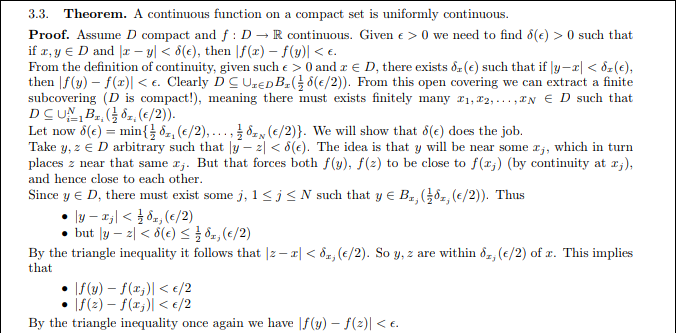
\includegraphics{figures/2019-12-19-16-49-56.png}\\
  \end{itemize}
\item
  Uniform convergence allows commuting sums with integrals
\item
  Closed subsets of compact sets are compact.
\item
  Every compact subset of a Hausdorff space is closed
\item
  Showing that a series converges: \emph{(Todo)}
\end{itemize}

\hypertarget{big-counterexamples}{%
\subsection{Big Counterexamples}\label{big-counterexamples}}

\hypertarget{for-limits}{%
\subsubsection{For Limits}\label{for-limits}}

\begin{itemize}
\item
  Differentiability \(\implies\) continuity but not the converse:

  \begin{itemize}
  \tightlist
  \item
    The Weierstrass function is continuous but nowhere differentiable.
  \end{itemize}
\item
  \(f\) continuous does not imply \(f'\) is continuous:
  \(f(x) = x^2 \sin(x)\).
\item
  Limit of derivatives may not equal derivative of limit:
  \begin{align*}
  f(x) = \frac{\sin(nx)}{n^c} \text{ where } 0 < c < 1.
  \end{align*}

  \begin{itemize}
  \tightlist
  \item
    Also shows that a sum of differentiable functions may not be
    differentiable.
  \end{itemize}
\item
  Limit of integrals may not equal integral of limit:
  \begin{align*}
  \sum \indic{x = q_n \in \QQ}
  .\end{align*}
\item
  A sequence of continuous functions converging to a discontinuous
  function:
  \begin{align*}
  f(x) = x^n \text{ on } [0, 1]
  .\end{align*}
\item
  The Thomae function \emph{(todo)}
\end{itemize}

\hypertarget{for-convergence}{%
\subsubsection{For Convergence}\label{for-convergence}}

\begin{itemize}
\tightlist
\item
  Notions of convergence:

  \begin{enumerate}
  \def\labelenumi{\arabic{enumi}.}
  \tightlist
  \item
    Uniform
  \item
    Pointwise
  \item
    Almost everywhere
  \item
    In norm
  \end{enumerate}
\end{itemize}

Uniform \(\implies\) pointwise \(\implies\) almost everywhere.

\begin{quote}
See Section 17.3.
\end{quote}

\hypertarget{almost-everywhere-convergence-does-not-imply-lp-convergence-for-any-1leq-p-leq-infty}{%
\paragraph{\texorpdfstring{Almost everywhere convergence does not imply
\(L^p\) convergence for any
\(1\leq p \leq \infty\)}{Almost everywhere convergence does not imply L\^{}p convergence for any 1\textbackslash leq p \textbackslash leq \textbackslash infty}}\label{almost-everywhere-convergence-does-not-imply-lp-convergence-for-any-1leq-p-leq-infty}}

\begin{quote}
See notes section 17.3.
\end{quote}

Sequences \(f_k \converges{a.e.}\to f\) but
\(f_k \converges{L^p}{\not\to} f\):

\begin{itemize}
\item
  For \(1\leq p < \infty\): The skateboard to infinity,
  \(f_k = \chi_{[k, k+1]}\).

  Then \(f_k \converges{a.e.}\to 0\) but \(\norm{f_k}_p = 1\) for all
  \(k\).

  \begin{quote}
  Converges pointwise and a.e., but not uniformly and not in norm.
  \end{quote}
\item
  For \(p = \infty\): The sliding boxes
  \(f_k = k \cdot \chi_{[0, \frac 1 k]}\).

  Then similarly \(f_k \converges{a.e.}\to 0\), but \(\norm{f_k}_p = 1\)
  and \(\norm{f_k}_\infty = k \to \infty\)

  \begin{quote}
  Converges a.e., but not uniformly, not pointwise, and not in norm.
  \end{quote}
\end{itemize}

\hypertarget{the-converse-to-the-dct-does-not-hold}{%
\paragraph{The Converse to the DCT does not
hold}\label{the-converse-to-the-dct-does-not-hold}}

\begin{quote}
\(L^p\) boundedness does not imply a.e. boundedness.
\end{quote}

I.e. it is not true that \(\lim \int f_k = \int f\) implies that
\(\exists g\in L^p\) such that \(f_k < g\) a.e. for every \(k\).

Take

\begin{itemize}
\item
  \(b_k = \sum_{j=1}^k \frac 1 j \to \infty\)
\item
  \(f_k = \chi_{[b_k, b_{k+1}]}\)
\end{itemize}

Then

\begin{itemize}
\item
  \(f_k \converges{a.e.}\to f = 0\),
\item
  \(\int f_k = \frac 1 k \to 0 \implies \norm{f_k}_p \to 0\),
\item
  \(0 = \int f = \lim \int f_k = 0\)
\item
  But \(g > f_k \implies g > \norm{f_k}_\infty = 1\) a.e.
  \(\implies g\not\in L^p(\RR)\).
\end{itemize}

\hypertarget{errata}{%
\subsection{Errata}\label{errata}}

\begin{itemize}
\tightlist
\item
  \textbf{Equicontinuity}: If \(\mathcal F \subset C(X)\) is a family of
  continuous functions on \(X\), then \(\mathcal F\)
  \emph{equicontinuous} at \(x\) iff
\end{itemize}

\begin{align*}
\forall \varepsilon > 0 ~~\exists U \ni x \text{ such that } y\in U \implies \abs{f(y) - f(x)} < \varepsilon \quad \forall f\in \mathcal{F}
.\end{align*}

\begin{itemize}
\item
  \textbf{Arzela - Ascoli 1}: If \(\mathcal{F}\) is pointwise bounded
  and equicontinuous, then \(\mathcal{F}\) is totally bounded in the
  uniform metric and its closure \(\overline{\mathcal{F}} \in C(X)\) in
  the space of continuous functions is compact.
\item
  \textbf{Arzela - Ascoli 2}: If \(\theset{f_k}\) is pointwise bounded
  and equicontinuous, then there exists a continuous \(f\) such that
  \(f_k \mapsvia{u} f\) on every compact set.
\end{itemize}

\textbf{Example:} Using Fatou to compute the limit of a sequence of
integrals:

\begin{align*}
\lim _{n \rightarrow \infty} \int_{0}^{\infty} \frac{n^{2}}{1+n^{2} x^{2}} e^{-\frac{x^{2}}{n^{3}}} d x
\overset{\text{Fatou}}\geq
\int_{0}^{\infty} \lim _{n \rightarrow \infty}  \frac{n^{2}}{1+n^{2} x^{2}} e^{-\frac{x^{2}}{n^{3}}} d x \to \int \infty
.\end{align*}

\begin{quote}
Note that MCT might work, but showing that this is non-decreasing in
\(n\) is difficult.
\end{quote}

\textbf{Lemma:} \begin{align*}
f_k \converges{a.e.}\to f ,\quad
\norm{f_k}_p \leq M
\implies f\in L^p \text{ and } \norm{f}_p \leq M
.\end{align*}

\begin{quote}
\emph{Proof:} Apply Fatou to \(\abs{f}^p\): \begin{align*}
\int \abs{f}^p = \int \liminf \abs{f_k}^p \leq \liminf \int \abs{f_k}^p = M
.\end{align*}
\end{quote}

\textbf{Lemma:} If \(f\) is uniformly continuous, then \begin{align*}
\norm{\tau_h f - f}_p \converges{L^p}\to 0 \quad \text{for all } p
.\end{align*}

\textbf{Lemma}: \(\norm{\tau_h f - f}_p \to 0\) for every \(p\).

\begin{quote}
\begin{itemize}
\tightlist
\item
  i.e.~``Continuity in \(L^1\)'' holds for all \(L^p\).
\item
  i.e.~Translation operators are continuous.
\end{itemize}
\end{quote}

\begin{quote}
\emph{Proof:} Take \(g_k \in C_c^0 \to f\), then \(g\) is uniformly
continuous, so \begin{align*}
\norm{\tau_h f - f}_p
\leq \norm{\tau_h f - \tau_h g}_p + \norm{\tau_h g - g}_p + \norm{g - f}_p \to 0
.\end{align*}
\end{quote}

\textbf{Lemma:} For \(f\in L^p, g\in L^q\), \(f\ast g\) is uniformly
continuous.

\begin{quote}
\emph{Proof}: Use Young's inequality \begin{align*}
\norm{\tau_h(f\ast g) - f\ast g}_\infty
&= \norm{(\tau_h f - f) \ast g}_\infty \leq \norm{\tau_hf - f}_p \norm{g}_q \to 0
.\end{align*}
\end{quote}

\textbf{Lemma}: If \(\int f \phi = 0\) for every \(\phi \in C_c^0\),
then \(f = 0\) almost everywhere.

\begin{quote}
\emph{Proof:} Let \(A\) be an interval, choose \(\phi_k \to \chi_A\),
then \(\int f \chi_A = 0\) for all intervals. So this holds for any
Borel set \(A\). Then just take \(A_1 = \theset{f > 0}\) and
\(A_2 = \theset{f < 0}\), then
\(\int_\RR f = \int_{A_1} f + \int_{A_2}f = 0\).
\end{quote}

\hypertarget{the-fourier-transform}{%
\subsection{The Fourier Transform}\label{the-fourier-transform}}

\textbf{Some Useful Properties:}

\begin{align*}
\widehat{f\ast g}(\xi)
&= \hat f(\xi) \cdot \hat g (\xi) \\
\widehat{\tau_h f}(\xi)
&= e^{2\pi i \xi \cdot h}\widehat{f}(\xi) \\
\widehat{e^{2\pi i \xi \cdot h}f(\xi)}
&= \tau_{-h}\widehat f(\xi) \\
\widehat{f \circ T}(\xi)
&= \abs{\det T}\inv (\hat f \circ T^{-t})(\xi) \\
\dd{}{\xi} \widehat{f}(\xi)
&= -2\pi i \cdot \widehat {\xi f} (\xi) \\
\widehat{\dd{}{\xi} f}(\xi)
&= 2\pi i \xi \cdot \widehat{f}(\xi)
.\end{align*}

\textbf{Some Useful Transform Pairs:}

\begin{align*}
\text{Dirichlet:}
&& \chi_{\theset{-\frac{1}{2} \leq x \leq \frac{1}{2}}}
&\iff \mathrm{sinc}(\xi) \\
\text{Fejer:}
&& \chi_{\theset{-1 \leq x \leq 1}} (1 - \abs{x})
&\iff \mathrm{sinc}^2(\xi) \\
\text{Poisson:}
&& \frac{1}{\pi} \frac{1}{1+x^2}
&\iff e^{2\pi \abs{\xi}} \\
\text{Gauss-Weierstrass:}
&& e^{-\pi x^2}
&\iff e^{-\pi \xi^2}
.\end{align*}

%\listoftodos

\bibliography{/home/zack/Notes/library.bib}

\end{document}
